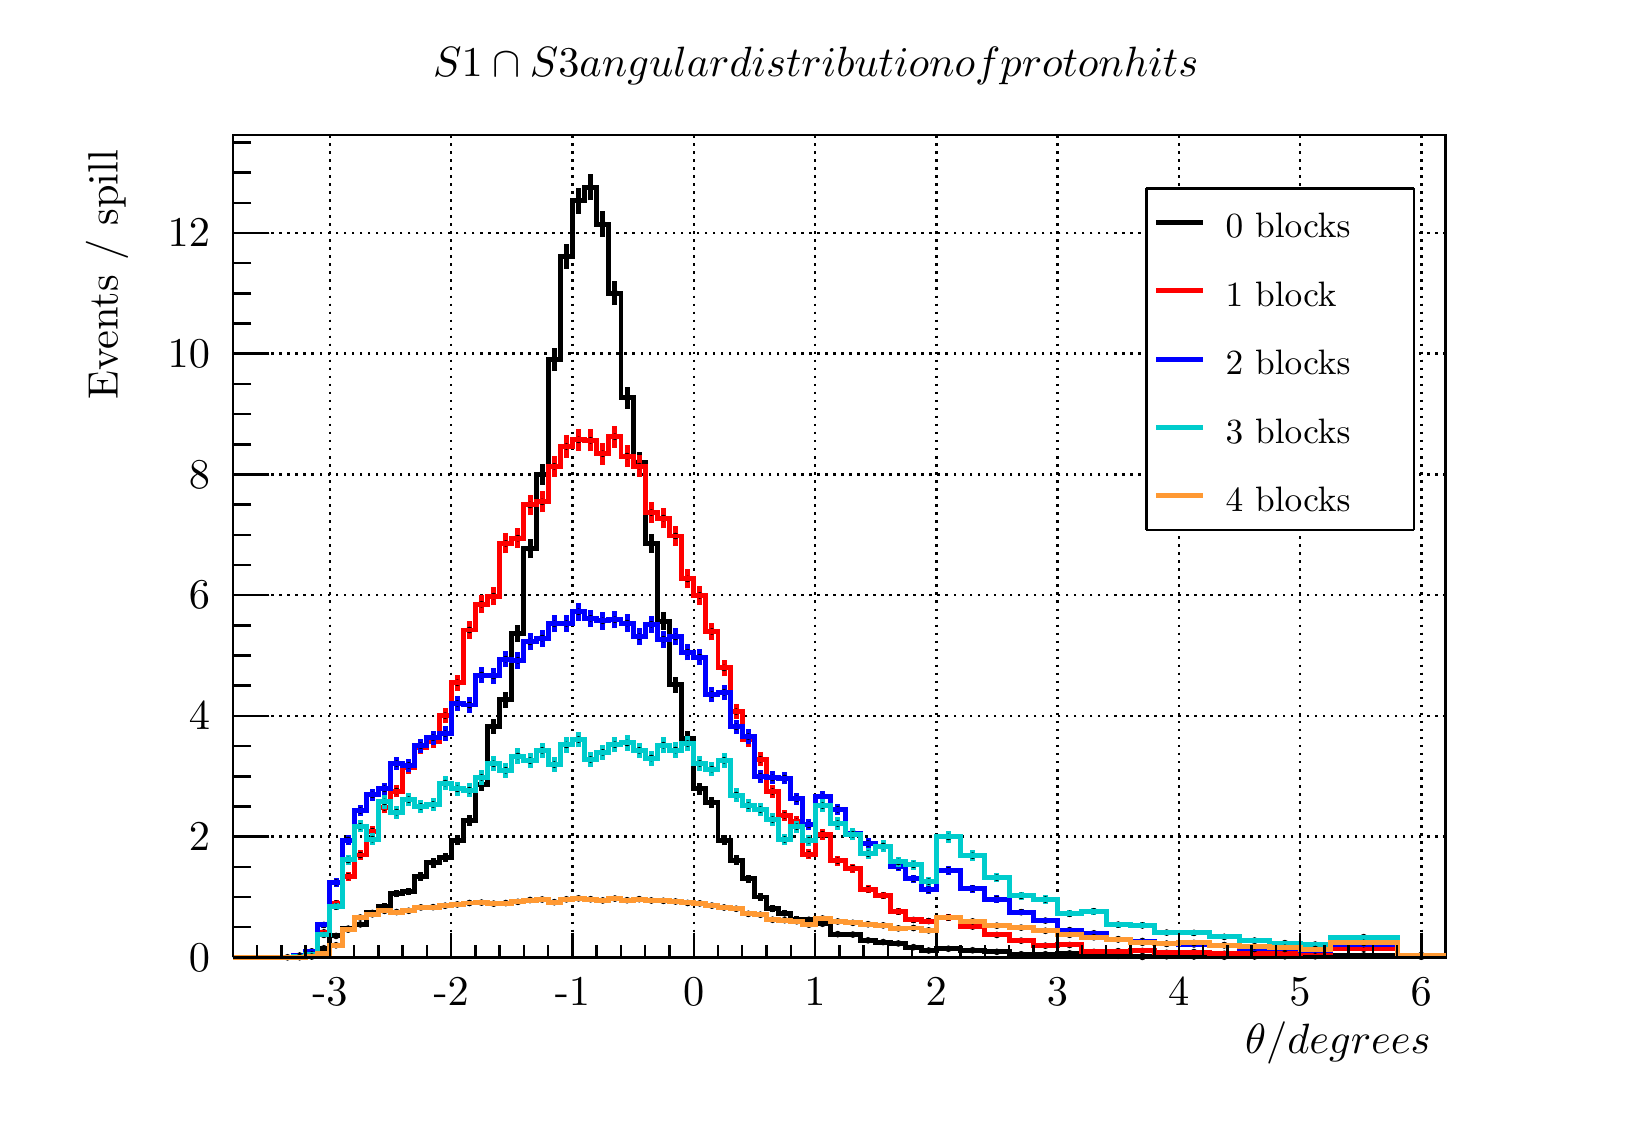
\begin{tikzpicture}
\pgfdeclareplotmark{cross} {
\pgfpathmoveto{\pgfpoint{-0.3\pgfplotmarksize}{\pgfplotmarksize}}
\pgfpathlineto{\pgfpoint{+0.3\pgfplotmarksize}{\pgfplotmarksize}}
\pgfpathlineto{\pgfpoint{+0.3\pgfplotmarksize}{0.3\pgfplotmarksize}}
\pgfpathlineto{\pgfpoint{+1\pgfplotmarksize}{0.3\pgfplotmarksize}}
\pgfpathlineto{\pgfpoint{+1\pgfplotmarksize}{-0.3\pgfplotmarksize}}
\pgfpathlineto{\pgfpoint{+0.3\pgfplotmarksize}{-0.3\pgfplotmarksize}}
\pgfpathlineto{\pgfpoint{+0.3\pgfplotmarksize}{-1.\pgfplotmarksize}}
\pgfpathlineto{\pgfpoint{-0.3\pgfplotmarksize}{-1.\pgfplotmarksize}}
\pgfpathlineto{\pgfpoint{-0.3\pgfplotmarksize}{-0.3\pgfplotmarksize}}
\pgfpathlineto{\pgfpoint{-1.\pgfplotmarksize}{-0.3\pgfplotmarksize}}
\pgfpathlineto{\pgfpoint{-1.\pgfplotmarksize}{0.3\pgfplotmarksize}}
\pgfpathlineto{\pgfpoint{-0.3\pgfplotmarksize}{0.3\pgfplotmarksize}}
\pgfpathclose
\pgfusepathqstroke
}
\pgfdeclareplotmark{cross*} {
\pgfpathmoveto{\pgfpoint{-0.3\pgfplotmarksize}{\pgfplotmarksize}}
\pgfpathlineto{\pgfpoint{+0.3\pgfplotmarksize}{\pgfplotmarksize}}
\pgfpathlineto{\pgfpoint{+0.3\pgfplotmarksize}{0.3\pgfplotmarksize}}
\pgfpathlineto{\pgfpoint{+1\pgfplotmarksize}{0.3\pgfplotmarksize}}
\pgfpathlineto{\pgfpoint{+1\pgfplotmarksize}{-0.3\pgfplotmarksize}}
\pgfpathlineto{\pgfpoint{+0.3\pgfplotmarksize}{-0.3\pgfplotmarksize}}
\pgfpathlineto{\pgfpoint{+0.3\pgfplotmarksize}{-1.\pgfplotmarksize}}
\pgfpathlineto{\pgfpoint{-0.3\pgfplotmarksize}{-1.\pgfplotmarksize}}
\pgfpathlineto{\pgfpoint{-0.3\pgfplotmarksize}{-0.3\pgfplotmarksize}}
\pgfpathlineto{\pgfpoint{-1.\pgfplotmarksize}{-0.3\pgfplotmarksize}}
\pgfpathlineto{\pgfpoint{-1.\pgfplotmarksize}{0.3\pgfplotmarksize}}
\pgfpathlineto{\pgfpoint{-0.3\pgfplotmarksize}{0.3\pgfplotmarksize}}
\pgfpathclose
\pgfusepathqfillstroke
}
\pgfdeclareplotmark{newstar} {
\pgfpathmoveto{\pgfqpoint{0pt}{\pgfplotmarksize}}
\pgfpathlineto{\pgfqpointpolar{44}{0.5\pgfplotmarksize}}
\pgfpathlineto{\pgfqpointpolar{18}{\pgfplotmarksize}}
\pgfpathlineto{\pgfqpointpolar{-20}{0.5\pgfplotmarksize}}
\pgfpathlineto{\pgfqpointpolar{-54}{\pgfplotmarksize}}
\pgfpathlineto{\pgfqpointpolar{-90}{0.5\pgfplotmarksize}}
\pgfpathlineto{\pgfqpointpolar{234}{\pgfplotmarksize}}
\pgfpathlineto{\pgfqpointpolar{198}{0.5\pgfplotmarksize}}
\pgfpathlineto{\pgfqpointpolar{162}{\pgfplotmarksize}}
\pgfpathlineto{\pgfqpointpolar{134}{0.5\pgfplotmarksize}}
\pgfpathclose
\pgfusepathqstroke
}
\pgfdeclareplotmark{newstar*} {
\pgfpathmoveto{\pgfqpoint{0pt}{\pgfplotmarksize}}
\pgfpathlineto{\pgfqpointpolar{44}{0.5\pgfplotmarksize}}
\pgfpathlineto{\pgfqpointpolar{18}{\pgfplotmarksize}}
\pgfpathlineto{\pgfqpointpolar{-20}{0.5\pgfplotmarksize}}
\pgfpathlineto{\pgfqpointpolar{-54}{\pgfplotmarksize}}
\pgfpathlineto{\pgfqpointpolar{-90}{0.5\pgfplotmarksize}}
\pgfpathlineto{\pgfqpointpolar{234}{\pgfplotmarksize}}
\pgfpathlineto{\pgfqpointpolar{198}{0.5\pgfplotmarksize}}
\pgfpathlineto{\pgfqpointpolar{162}{\pgfplotmarksize}}
\pgfpathlineto{\pgfqpointpolar{134}{0.5\pgfplotmarksize}}
\pgfpathclose
\pgfusepathqfillstroke
}
\definecolor{c}{rgb}{1,1,1};
\draw [color=c, fill=c] (0,0) rectangle (20,13.5632);
\draw [color=c, fill=c] (2.6,1.76322) rectangle (18,12.2069);
\definecolor{c}{rgb}{0,0,0};
\draw [c,line width=0.9] (2.6,1.76322) -- (2.6,12.2069) -- (18,12.2069) -- (18,1.76322) -- (2.6,1.76322);
\definecolor{c}{rgb}{1,1,1};
\draw [color=c, fill=c] (2.6,1.76322) rectangle (18,12.2069);
\definecolor{c}{rgb}{0,0,0};
\draw [c,line width=0.9] (2.6,1.76322) -- (2.6,12.2069) -- (18,12.2069) -- (18,1.76322) -- (2.6,1.76322);
\draw [c,line width=0.9] (2.6,1.76322) -- (18,1.76322);
\draw [c,dotted,line width=0.9] (3.832,12.2069) -- (3.832,1.76322);
\draw [c,dotted,line width=0.9] (5.372,12.2069) -- (5.372,1.76322);
\draw [c,dotted,line width=0.9] (6.912,12.2069) -- (6.912,1.76322);
\draw [c,dotted,line width=0.9] (8.452,12.2069) -- (8.452,1.76322);
\draw [c,dotted,line width=0.9] (9.992,12.2069) -- (9.992,1.76322);
\draw [c,dotted,line width=0.9] (11.532,12.2069) -- (11.532,1.76322);
\draw [c,dotted,line width=0.9] (13.072,12.2069) -- (13.072,1.76322);
\draw [c,dotted,line width=0.9] (14.612,12.2069) -- (14.612,1.76322);
\draw [c,dotted,line width=0.9] (16.152,12.2069) -- (16.152,1.76322);
\draw [c,dotted,line width=0.9] (17.692,12.2069) -- (17.692,1.76322);
\draw [c,dotted,line width=0.9] (3.832,12.2069) -- (3.832,1.76322);
\draw [c,dotted,line width=0.9] (17.692,12.2069) -- (17.692,1.76322);
\draw [c,line width=0.9] (2.6,1.76322) -- (2.6,12.2069);
\draw [c,dotted,line width=0.9] (18,1.76322) -- (2.6,1.76322);
\draw [c,dotted,line width=0.9] (18,3.29644) -- (2.6,3.29644);
\draw [c,dotted,line width=0.9] (18,4.82967) -- (2.6,4.82967);
\draw [c,dotted,line width=0.9] (18,6.3629) -- (2.6,6.3629);
\draw [c,dotted,line width=0.9] (18,7.89612) -- (2.6,7.89612);
\draw [c,dotted,line width=0.9] (18,9.42935) -- (2.6,9.42935);
\draw [c,dotted,line width=0.9] (18,10.9626) -- (2.6,10.9626);
\draw [c,dotted,line width=0.9] (18,10.9626) -- (2.6,10.9626);
\definecolor{c}{rgb}{0,0,0.6};
\draw [c,line width=0.9] (2.6,1.76322) -- (2.754,1.76322) -- (2.754,1.76322) -- (2.908,1.76322) -- (2.908,1.76322) -- (3.062,1.76322) -- (3.062,1.76322) -- (3.216,1.76322) -- (3.216,1.76322) -- (3.37,1.76322) -- (3.37,1.76322) -- (3.524,1.76322) --
 (3.524,1.76322) -- (3.678,1.76322) -- (3.678,1.76322) -- (3.832,1.76322) -- (3.832,1.76322) -- (3.986,1.76322) -- (3.986,1.76322) -- (4.14,1.76322) -- (4.14,1.76322) -- (4.294,1.76322) -- (4.294,1.76322) -- (4.448,1.76322) -- (4.448,1.76322) --
 (4.602,1.76322) -- (4.602,1.76322) -- (4.756,1.76322) -- (4.756,1.76322) -- (4.91,1.76322) -- (4.91,1.76322) -- (5.064,1.76322) -- (5.064,1.76322) -- (5.218,1.76322) -- (5.218,1.76322) -- (5.372,1.76322) -- (5.372,1.76322) -- (5.526,1.76322) --
 (5.526,1.76322) -- (5.68,1.76322) -- (5.68,1.76322) -- (5.834,1.76322) -- (5.834,1.76322) -- (5.988,1.76322) -- (5.988,1.76322) -- (6.142,1.76322) -- (6.142,1.76322) -- (6.296,1.76322) -- (6.296,1.76322) -- (6.45,1.76322) -- (6.45,1.76322) --
 (6.604,1.76322) -- (6.604,1.76322) -- (6.758,1.76322) -- (6.758,1.76322) -- (6.912,1.76322) -- (6.912,1.76322) -- (7.066,1.76322) -- (7.066,1.76322) -- (7.22,1.76322) -- (7.22,1.76322) -- (7.374,1.76322) -- (7.374,1.76322) -- (7.528,1.76322) --
 (7.528,1.76322) -- (7.682,1.76322) -- (7.682,1.76322) -- (7.836,1.76322) -- (7.836,1.76322) -- (7.99,1.76322) -- (7.99,1.76322) -- (8.144,1.76322) -- (8.144,1.76322) -- (8.298,1.76322) -- (8.298,1.76322) -- (8.452,1.76322) -- (8.452,1.76322) --
 (8.606,1.76322) -- (8.606,1.76322) -- (8.76,1.76322) -- (8.76,1.76322) -- (8.914,1.76322) -- (8.914,1.76322) -- (9.068,1.76322) -- (9.068,1.76322) -- (9.222,1.76322) -- (9.222,1.76322) -- (9.376,1.76322) -- (9.376,1.76322) -- (9.53,1.76322) --
 (9.53,1.76322) -- (9.684,1.76322) -- (9.684,1.76322) -- (9.838,1.76322) -- (9.838,1.76322) -- (9.992,1.76322) -- (9.992,1.76322) -- (10.1845,1.76322) -- (10.1845,1.76322) -- (10.377,1.76322) -- (10.377,1.76322) -- (10.5695,1.76322) --
 (10.5695,1.76322) -- (10.762,1.76322) -- (10.762,1.76322) -- (10.9545,1.76322) -- (10.9545,1.76322) -- (11.147,1.76322) -- (11.147,1.76322) -- (11.3395,1.76322) -- (11.3395,1.76322) -- (11.532,1.76322) -- (11.532,1.76322) -- (11.84,1.76322) --
 (11.84,1.76322) -- (12.148,1.76322) -- (12.148,1.76322) -- (12.456,1.76322) -- (12.456,1.76322) -- (12.764,1.76322) -- (12.764,1.76322) -- (13.072,1.76322) -- (13.072,1.76322) -- (13.38,1.76322) -- (13.38,1.76322) -- (13.688,1.76322) --
 (13.688,1.76322) -- (13.996,1.76322) -- (13.996,1.76322) -- (14.304,1.76322) -- (14.304,1.76322) -- (14.612,1.76322) -- (14.612,1.76322) -- (14.997,1.76322) -- (14.997,1.76322) -- (15.382,1.76322) -- (15.382,1.76322) -- (15.767,1.76322) --
 (15.767,1.76322) -- (16.152,1.76322) -- (16.152,1.76322) -- (16.537,1.76322) -- (16.537,1.76322) -- (17.384,1.76322) -- (17.384,1.76322) -- (18,1.76322);
\definecolor{c}{rgb}{0,0,0};
\draw [c,line width=0.9] (2.6,1.76322) -- (18,1.76322);
\draw [anchor= east] (18,0.678161) node[scale=1.5317, color=c, rotate=0]{$ \theta / degrees$};
\draw [c,line width=0.9] (3.832,2.07653) -- (3.832,1.76322);
\draw [c,line width=0.9] (4.14,1.91987) -- (4.14,1.76322);
\draw [c,line width=0.9] (4.448,1.91987) -- (4.448,1.76322);
\draw [c,line width=0.9] (4.756,1.91987) -- (4.756,1.76322);
\draw [c,line width=0.9] (5.064,1.91987) -- (5.064,1.76322);
\draw [c,line width=0.9] (5.372,2.07653) -- (5.372,1.76322);
\draw [c,line width=0.9] (5.68,1.91987) -- (5.68,1.76322);
\draw [c,line width=0.9] (5.988,1.91987) -- (5.988,1.76322);
\draw [c,line width=0.9] (6.296,1.91987) -- (6.296,1.76322);
\draw [c,line width=0.9] (6.604,1.91987) -- (6.604,1.76322);
\draw [c,line width=0.9] (6.912,2.07653) -- (6.912,1.76322);
\draw [c,line width=0.9] (7.22,1.91987) -- (7.22,1.76322);
\draw [c,line width=0.9] (7.528,1.91987) -- (7.528,1.76322);
\draw [c,line width=0.9] (7.836,1.91987) -- (7.836,1.76322);
\draw [c,line width=0.9] (8.144,1.91987) -- (8.144,1.76322);
\draw [c,line width=0.9] (8.452,2.07653) -- (8.452,1.76322);
\draw [c,line width=0.9] (8.76,1.91987) -- (8.76,1.76322);
\draw [c,line width=0.9] (9.068,1.91987) -- (9.068,1.76322);
\draw [c,line width=0.9] (9.376,1.91987) -- (9.376,1.76322);
\draw [c,line width=0.9] (9.684,1.91987) -- (9.684,1.76322);
\draw [c,line width=0.9] (9.992,2.07653) -- (9.992,1.76322);
\draw [c,line width=0.9] (10.3,1.91987) -- (10.3,1.76322);
\draw [c,line width=0.9] (10.608,1.91987) -- (10.608,1.76322);
\draw [c,line width=0.9] (10.916,1.91987) -- (10.916,1.76322);
\draw [c,line width=0.9] (11.224,1.91987) -- (11.224,1.76322);
\draw [c,line width=0.9] (11.532,2.07653) -- (11.532,1.76322);
\draw [c,line width=0.9] (11.84,1.91987) -- (11.84,1.76322);
\draw [c,line width=0.9] (12.148,1.91987) -- (12.148,1.76322);
\draw [c,line width=0.9] (12.456,1.91987) -- (12.456,1.76322);
\draw [c,line width=0.9] (12.764,1.91987) -- (12.764,1.76322);
\draw [c,line width=0.9] (13.072,2.07653) -- (13.072,1.76322);
\draw [c,line width=0.9] (13.38,1.91987) -- (13.38,1.76322);
\draw [c,line width=0.9] (13.688,1.91987) -- (13.688,1.76322);
\draw [c,line width=0.9] (13.996,1.91987) -- (13.996,1.76322);
\draw [c,line width=0.9] (14.304,1.91987) -- (14.304,1.76322);
\draw [c,line width=0.9] (14.612,2.07653) -- (14.612,1.76322);
\draw [c,line width=0.9] (14.92,1.91987) -- (14.92,1.76322);
\draw [c,line width=0.9] (15.228,1.91987) -- (15.228,1.76322);
\draw [c,line width=0.9] (15.536,1.91987) -- (15.536,1.76322);
\draw [c,line width=0.9] (15.844,1.91987) -- (15.844,1.76322);
\draw [c,line width=0.9] (16.152,2.07653) -- (16.152,1.76322);
\draw [c,line width=0.9] (16.46,1.91987) -- (16.46,1.76322);
\draw [c,line width=0.9] (16.768,1.91987) -- (16.768,1.76322);
\draw [c,line width=0.9] (17.076,1.91987) -- (17.076,1.76322);
\draw [c,line width=0.9] (17.384,1.91987) -- (17.384,1.76322);
\draw [c,line width=0.9] (17.692,2.07653) -- (17.692,1.76322);
\draw [c,line width=0.9] (3.832,2.07653) -- (3.832,1.76322);
\draw [c,line width=0.9] (3.524,1.91987) -- (3.524,1.76322);
\draw [c,line width=0.9] (3.216,1.91987) -- (3.216,1.76322);
\draw [c,line width=0.9] (2.908,1.91987) -- (2.908,1.76322);
\draw [c,line width=0.9] (17.692,2.07653) -- (17.692,1.76322);
\draw [anchor=base] (3.832,1.15287) node[scale=1.5317, color=c, rotate=0]{-3};
\draw [anchor=base] (5.372,1.15287) node[scale=1.5317, color=c, rotate=0]{-2};
\draw [anchor=base] (6.912,1.15287) node[scale=1.5317, color=c, rotate=0]{-1};
\draw [anchor=base] (8.452,1.15287) node[scale=1.5317, color=c, rotate=0]{0};
\draw [anchor=base] (9.992,1.15287) node[scale=1.5317, color=c, rotate=0]{1};
\draw [anchor=base] (11.532,1.15287) node[scale=1.5317, color=c, rotate=0]{2};
\draw [anchor=base] (13.072,1.15287) node[scale=1.5317, color=c, rotate=0]{3};
\draw [anchor=base] (14.612,1.15287) node[scale=1.5317, color=c, rotate=0]{4};
\draw [anchor=base] (16.152,1.15287) node[scale=1.5317, color=c, rotate=0]{5};
\draw [anchor=base] (17.692,1.15287) node[scale=1.5317, color=c, rotate=0]{6};
\draw [c,line width=0.9] (2.6,1.76322) -- (2.6,12.2069);
\draw [anchor= east] (1,12.2069) node[scale=1.5317, color=c, rotate=90]{ Events / spill};
\draw [c,line width=0.9] (3.062,1.76322) -- (2.6,1.76322);
\draw [c,line width=0.9] (2.831,2.14652) -- (2.6,2.14652);
\draw [c,line width=0.9] (2.831,2.52983) -- (2.6,2.52983);
\draw [c,line width=0.9] (2.831,2.91314) -- (2.6,2.91314);
\draw [c,line width=0.9] (3.062,3.29644) -- (2.6,3.29644);
\draw [c,line width=0.9] (2.831,3.67975) -- (2.6,3.67975);
\draw [c,line width=0.9] (2.831,4.06306) -- (2.6,4.06306);
\draw [c,line width=0.9] (2.831,4.44636) -- (2.6,4.44636);
\draw [c,line width=0.9] (3.062,4.82967) -- (2.6,4.82967);
\draw [c,line width=0.9] (2.831,5.21298) -- (2.6,5.21298);
\draw [c,line width=0.9] (2.831,5.59628) -- (2.6,5.59628);
\draw [c,line width=0.9] (2.831,5.97959) -- (2.6,5.97959);
\draw [c,line width=0.9] (3.062,6.3629) -- (2.6,6.3629);
\draw [c,line width=0.9] (2.831,6.7462) -- (2.6,6.7462);
\draw [c,line width=0.9] (2.831,7.12951) -- (2.6,7.12951);
\draw [c,line width=0.9] (2.831,7.51282) -- (2.6,7.51282);
\draw [c,line width=0.9] (3.062,7.89612) -- (2.6,7.89612);
\draw [c,line width=0.9] (2.831,8.27943) -- (2.6,8.27943);
\draw [c,line width=0.9] (2.831,8.66273) -- (2.6,8.66273);
\draw [c,line width=0.9] (2.831,9.04604) -- (2.6,9.04604);
\draw [c,line width=0.9] (3.062,9.42935) -- (2.6,9.42935);
\draw [c,line width=0.9] (2.831,9.81265) -- (2.6,9.81265);
\draw [c,line width=0.9] (2.831,10.196) -- (2.6,10.196);
\draw [c,line width=0.9] (2.831,10.5793) -- (2.6,10.5793);
\draw [c,line width=0.9] (3.062,10.9626) -- (2.6,10.9626);
\draw [c,line width=0.9] (3.062,10.9626) -- (2.6,10.9626);
\draw [c,line width=0.9] (2.831,11.3459) -- (2.6,11.3459);
\draw [c,line width=0.9] (2.831,11.7292) -- (2.6,11.7292);
\draw [c,line width=0.9] (2.831,12.1125) -- (2.6,12.1125);
\draw [anchor= east] (2.5,1.76322) node[scale=1.5317, color=c, rotate=0]{0};
\draw [anchor= east] (2.5,3.29644) node[scale=1.5317, color=c, rotate=0]{2};
\draw [anchor= east] (2.5,4.82967) node[scale=1.5317, color=c, rotate=0]{4};
\draw [anchor= east] (2.5,6.3629) node[scale=1.5317, color=c, rotate=0]{6};
\draw [anchor= east] (2.5,7.89612) node[scale=1.5317, color=c, rotate=0]{8};
\draw [anchor= east] (2.5,9.42935) node[scale=1.5317, color=c, rotate=0]{10};
\draw [anchor= east] (2.5,10.9626) node[scale=1.5317, color=c, rotate=0]{12};
\draw [c,line width=1.8] (3.447,1.76678) -- (3.447,1.77164);
\draw [c,line width=1.8] (3.447,1.77164) -- (3.447,1.77651);
\foreach \P in {(3.447,1.77164)}{\draw[mark options={color=c,fill=c},mark size=2.402402pt,mark=*,mark size=1pt] plot coordinates {\P};}
\draw [c,line width=1.8] (3.601,1.78719) -- (3.601,1.79692);
\draw [c,line width=1.8] (3.601,1.79692) -- (3.601,1.80664);
\foreach \P in {(3.601,1.79692)}{\draw[mark options={color=c,fill=c},mark size=2.402402pt,mark=*,mark size=1pt] plot coordinates {\P};}
\draw [c,line width=1.8] (3.755,1.86037) -- (3.755,1.87835);
\draw [c,line width=1.8] (3.755,1.87835) -- (3.755,1.89633);
\foreach \P in {(3.755,1.87835)}{\draw[mark options={color=c,fill=c},mark size=2.402402pt,mark=*,mark size=1pt] plot coordinates {\P};}
\draw [c,line width=1.8] (3.909,2.00795) -- (3.909,2.0356);
\draw [c,line width=1.8] (3.909,2.0356) -- (3.909,2.06326);
\foreach \P in {(3.909,2.0356)}{\draw[mark options={color=c,fill=c},mark size=2.402402pt,mark=*,mark size=1pt] plot coordinates {\P};}
\draw [c,line width=1.8] (4.063,2.09625) -- (4.063,2.12827);
\draw [c,line width=1.8] (4.063,2.12827) -- (4.063,2.16029);
\foreach \P in {(4.063,2.12827)}{\draw[mark options={color=c,fill=c},mark size=2.402402pt,mark=*,mark size=1pt] plot coordinates {\P};}
\draw [c,line width=1.8] (4.217,2.14735) -- (4.217,2.18163);
\draw [c,line width=1.8] (4.217,2.18163) -- (4.217,2.2159);
\foreach \P in {(4.217,2.18163)}{\draw[mark options={color=c,fill=c},mark size=2.402402pt,mark=*,mark size=1pt] plot coordinates {\P};}
\draw [c,line width=1.8] (4.371,2.28784) -- (4.371,2.32765);
\draw [c,line width=1.8] (4.371,2.32765) -- (4.371,2.36746);
\foreach \P in {(4.371,2.32765)}{\draw[mark options={color=c,fill=c},mark size=2.402402pt,mark=*,mark size=1pt] plot coordinates {\P};}
\draw [c,line width=1.8] (4.525,2.36378) -- (4.525,2.40627);
\draw [c,line width=1.8] (4.525,2.40627) -- (4.525,2.44877);
\foreach \P in {(4.525,2.40627)}{\draw[mark options={color=c,fill=c},mark size=2.402402pt,mark=*,mark size=1pt] plot coordinates {\P};}
\draw [c,line width=1.8] (4.679,2.5243) -- (4.679,2.57195);
\draw [c,line width=1.8] (4.679,2.57195) -- (4.679,2.61961);
\foreach \P in {(4.679,2.57195)}{\draw[mark options={color=c,fill=c},mark size=2.402402pt,mark=*,mark size=1pt] plot coordinates {\P};}
\draw [c,line width=1.8] (4.833,2.54883) -- (4.833,2.59723);
\draw [c,line width=1.8] (4.833,2.59723) -- (4.833,2.64562);
\foreach \P in {(4.833,2.59723)}{\draw[mark options={color=c,fill=c},mark size=2.402402pt,mark=*,mark size=1pt] plot coordinates {\P};}
\draw [c,line width=1.8] (4.987,2.73453) -- (4.987,2.78818);
\draw [c,line width=1.8] (4.987,2.78818) -- (4.987,2.84183);
\foreach \P in {(4.987,2.78818)}{\draw[mark options={color=c,fill=c},mark size=2.402402pt,mark=*,mark size=1pt] plot coordinates {\P};}
\draw [c,line width=1.8] (5.141,2.90425) -- (5.141,2.96228);
\draw [c,line width=1.8] (5.141,2.96228) -- (5.141,3.02031);
\foreach \P in {(5.141,2.96228)}{\draw[mark options={color=c,fill=c},mark size=2.402402pt,mark=*,mark size=1pt] plot coordinates {\P};}
\draw [c,line width=1.8] (5.295,2.97278) -- (5.295,3.03248);
\draw [c,line width=1.8] (5.295,3.03248) -- (5.295,3.09218);
\foreach \P in {(5.295,3.03248)}{\draw[mark options={color=c,fill=c},mark size=2.402402pt,mark=*,mark size=1pt] plot coordinates {\P};}
\draw [c,line width=1.8] (5.449,3.18412) -- (5.449,3.24871);
\draw [c,line width=1.8] (5.449,3.24871) -- (5.449,3.31329);
\foreach \P in {(5.449,3.24871)}{\draw[mark options={color=c,fill=c},mark size=2.402402pt,mark=*,mark size=1pt] plot coordinates {\P};}
\draw [c,line width=1.8] (5.603,3.43432) -- (5.603,3.50424);
\draw [c,line width=1.8] (5.603,3.50424) -- (5.603,3.57417);
\foreach \P in {(5.603,3.50424)}{\draw[mark options={color=c,fill=c},mark size=2.402402pt,mark=*,mark size=1pt] plot coordinates {\P};}
\draw [c,line width=1.8] (5.757,3.87787) -- (5.757,3.95635);
\draw [c,line width=1.8] (5.757,3.95635) -- (5.757,4.03483);
\foreach \P in {(5.757,3.95635)}{\draw[mark options={color=c,fill=c},mark size=2.402402pt,mark=*,mark size=1pt] plot coordinates {\P};}
\draw [c,line width=1.8] (5.911,4.60415) -- (5.911,4.69488);
\draw [c,line width=1.8] (5.911,4.69488) -- (5.911,4.78561);
\foreach \P in {(5.911,4.69488)}{\draw[mark options={color=c,fill=c},mark size=2.402402pt,mark=*,mark size=1pt] plot coordinates {\P};}
\draw [c,line width=1.8] (6.065,4.93605) -- (6.065,5.03185);
\draw [c,line width=1.8] (6.065,5.03185) -- (6.065,5.12766);
\foreach \P in {(6.065,5.03185)}{\draw[mark options={color=c,fill=c},mark size=2.402402pt,mark=*,mark size=1pt] plot coordinates {\P};}
\draw [c,line width=1.8] (6.219,5.76684) -- (6.219,5.87429);
\draw [c,line width=1.8] (6.219,5.87429) -- (6.219,5.98173);
\foreach \P in {(6.219,5.87429)}{\draw[mark options={color=c,fill=c},mark size=2.402402pt,mark=*,mark size=1pt] plot coordinates {\P};}
\draw [c,line width=1.8] (6.373,6.82911) -- (6.373,6.94979);
\draw [c,line width=1.8] (6.373,6.94979) -- (6.373,7.07047);
\foreach \P in {(6.373,6.94979)}{\draw[mark options={color=c,fill=c},mark size=2.402402pt,mark=*,mark size=1pt] plot coordinates {\P};}
\draw [c,line width=1.8] (6.527,7.76767) -- (6.527,7.89893);
\draw [c,line width=1.8] (6.527,7.89893) -- (6.527,8.03019);
\foreach \P in {(6.527,7.89893)}{\draw[mark options={color=c,fill=c},mark size=2.402402pt,mark=*,mark size=1pt] plot coordinates {\P};}
\draw [c,line width=1.8] (6.681,9.20753) -- (6.681,9.35353);
\draw [c,line width=1.8] (6.681,9.35353) -- (6.681,9.49952);
\foreach \P in {(6.681,9.35353)}{\draw[mark options={color=c,fill=c},mark size=2.402402pt,mark=*,mark size=1pt] plot coordinates {\P};}
\draw [c,line width=1.8] (6.835,10.5096) -- (6.835,10.6677);
\draw [c,line width=1.8] (6.835,10.6677) -- (6.835,10.8259);
\foreach \P in {(6.835,10.6677)}{\draw[mark options={color=c,fill=c},mark size=2.402402pt,mark=*,mark size=1pt] plot coordinates {\P};}
\draw [c,line width=1.8] (6.989,11.2055) -- (6.989,11.3698);
\draw [c,line width=1.8] (6.989,11.3698) -- (6.989,11.534);
\foreach \P in {(6.989,11.3698)}{\draw[mark options={color=c,fill=c},mark size=2.402402pt,mark=*,mark size=1pt] plot coordinates {\P};}
\draw [c,line width=1.8] (7.143,11.3781) -- (7.143,11.5439);
\draw [c,line width=1.8] (7.143,11.5439) -- (7.143,11.7096);
\foreach \P in {(7.143,11.5439)}{\draw[mark options={color=c,fill=c},mark size=2.402402pt,mark=*,mark size=1pt] plot coordinates {\P};}
\draw [c,line width=1.8] (7.297,10.9132) -- (7.297,11.0749);
\draw [c,line width=1.8] (7.297,11.0749) -- (7.297,11.2366);
\foreach \P in {(7.297,11.0749)}{\draw[mark options={color=c,fill=c},mark size=2.402402pt,mark=*,mark size=1pt] plot coordinates {\P};}
\draw [c,line width=1.8] (7.451,10.0449) -- (7.451,10.1988);
\draw [c,line width=1.8] (7.451,10.1988) -- (7.451,10.3527);
\foreach \P in {(7.451,10.1988)}{\draw[mark options={color=c,fill=c},mark size=2.402402pt,mark=*,mark size=1pt] plot coordinates {\P};}
\draw [c,line width=1.8] (7.605,8.72926) -- (7.605,8.87053);
\draw [c,line width=1.8] (7.605,8.87053) -- (7.605,9.01181);
\foreach \P in {(7.605,8.87053)}{\draw[mark options={color=c,fill=c},mark size=2.402402pt,mark=*,mark size=1pt] plot coordinates {\P};}
\draw [c,line width=1.8] (7.759,7.92047) -- (7.759,8.05338);
\draw [c,line width=1.8] (7.759,8.05338) -- (7.759,8.18628);
\foreach \P in {(7.759,8.05338)}{\draw[mark options={color=c,fill=c},mark size=2.402402pt,mark=*,mark size=1pt] plot coordinates {\P};}
\draw [c,line width=1.8] (7.913,6.90127) -- (7.913,7.0228);
\draw [c,line width=1.8] (7.913,7.0228) -- (7.913,7.14433);
\foreach \P in {(7.913,7.0228)}{\draw[mark options={color=c,fill=c},mark size=2.402402pt,mark=*,mark size=1pt] plot coordinates {\P};}
\draw [c,line width=1.8] (8.067,5.92483) -- (8.067,6.03435);
\draw [c,line width=1.8] (8.067,6.03435) -- (8.067,6.14386);
\foreach \P in {(8.067,6.03435)}{\draw[mark options={color=c,fill=c},mark size=2.402402pt,mark=*,mark size=1pt] plot coordinates {\P};}
\draw [c,line width=1.8] (8.221,5.12424) -- (8.221,5.22281);
\draw [c,line width=1.8] (8.221,5.22281) -- (8.221,5.32137);
\foreach \P in {(8.221,5.22281)}{\draw[mark options={color=c,fill=c},mark size=2.402402pt,mark=*,mark size=1pt] plot coordinates {\P};}
\draw [c,line width=1.8] (8.375,4.46042) -- (8.375,4.54886);
\draw [c,line width=1.8] (8.375,4.54886) -- (8.375,4.6373);
\foreach \P in {(8.375,4.54886)}{\draw[mark options={color=c,fill=c},mark size=2.402402pt,mark=*,mark size=1pt] plot coordinates {\P};}
\draw [c,line width=1.8] (8.529,3.82548) -- (8.529,3.903);
\draw [c,line width=1.8] (8.529,3.903) -- (8.529,3.98051);
\foreach \P in {(8.529,3.903)}{\draw[mark options={color=c,fill=c},mark size=2.402402pt,mark=*,mark size=1pt] plot coordinates {\P};}
\draw [c,line width=1.8] (8.683,3.65735) -- (8.683,3.7317);
\draw [c,line width=1.8] (8.683,3.7317) -- (8.683,3.80605);
\foreach \P in {(8.683,3.7317)}{\draw[mark options={color=c,fill=c},mark size=2.402402pt,mark=*,mark size=1pt] plot coordinates {\P};}
\draw [c,line width=1.8] (8.837,3.18412) -- (8.837,3.24871);
\draw [c,line width=1.8] (8.837,3.24871) -- (8.837,3.31329);
\foreach \P in {(8.837,3.24871)}{\draw[mark options={color=c,fill=c},mark size=2.402402pt,mark=*,mark size=1pt] plot coordinates {\P};}
\draw [c,line width=1.8] (8.991,2.93988) -- (8.991,2.99879);
\draw [c,line width=1.8] (8.991,2.99879) -- (8.991,3.05769);
\foreach \P in {(8.991,2.99879)}{\draw[mark options={color=c,fill=c},mark size=2.402402pt,mark=*,mark size=1pt] plot coordinates {\P};}
\draw [c,line width=1.8] (9.145,2.70719) -- (9.145,2.7601);
\draw [c,line width=1.8] (9.145,2.7601) -- (9.145,2.813);
\foreach \P in {(9.145,2.7601)}{\draw[mark options={color=c,fill=c},mark size=2.402402pt,mark=*,mark size=1pt] plot coordinates {\P};}
\draw [c,line width=1.8] (9.299,2.48343) -- (9.299,2.52983);
\draw [c,line width=1.8] (9.299,2.52983) -- (9.299,2.57623);
\foreach \P in {(9.299,2.52983)}{\draw[mark options={color=c,fill=c},mark size=2.402402pt,mark=*,mark size=1pt] plot coordinates {\P};}
\draw [c,line width=1.8] (9.453,2.33935) -- (9.453,2.381);
\draw [c,line width=1.8] (9.453,2.381) -- (9.453,2.42265);
\foreach \P in {(9.453,2.381)}{\draw[mark options={color=c,fill=c},mark size=2.402402pt,mark=*,mark size=1pt] plot coordinates {\P};}
\draw [c,line width=1.8] (9.607,2.28242) -- (9.607,2.32203);
\draw [c,line width=1.8] (9.607,2.32203) -- (9.607,2.36164);
\foreach \P in {(9.607,2.32203)}{\draw[mark options={color=c,fill=c},mark size=2.402402pt,mark=*,mark size=1pt] plot coordinates {\P};}
\draw [c,line width=1.8] (9.761,2.20938) -- (9.761,2.24621);
\draw [c,line width=1.8] (9.761,2.24621) -- (9.761,2.28304);
\foreach \P in {(9.761,2.24621)}{\draw[mark options={color=c,fill=c},mark size=2.402402pt,mark=*,mark size=1pt] plot coordinates {\P};}
\draw [c,line width=1.8] (9.915,2.20398) -- (9.915,2.2406);
\draw [c,line width=1.8] (9.915,2.2406) -- (9.915,2.27721);
\foreach \P in {(9.915,2.2406)}{\draw[mark options={color=c,fill=c},mark size=2.402402pt,mark=*,mark size=1pt] plot coordinates {\P};}
\draw [c,line width=1.8] (10.0883,2.15543) -- (10.0883,2.19005);
\draw [c,line width=1.8] (10.0883,2.19005) -- (10.0883,2.22467);
\foreach \P in {(10.0883,2.19005)}{\draw[mark options={color=c,fill=c},mark size=2.402402pt,mark=*,mark size=1pt] plot coordinates {\P};}
\draw [c,line width=1.8] (10.2808,2.02929) -- (10.2808,2.05807);
\draw [c,line width=1.8] (10.2808,2.05807) -- (10.2808,2.08684);
\foreach \P in {(10.2808,2.05807)}{\draw[mark options={color=c,fill=c},mark size=2.402402pt,mark=*,mark size=1pt] plot coordinates {\P};}
\draw [c,line width=1.8] (10.4733,2.02395) -- (10.4733,2.05245);
\draw [c,line width=1.8] (10.4733,2.05245) -- (10.4733,2.08095);
\foreach \P in {(10.4733,2.05245)}{\draw[mark options={color=c,fill=c},mark size=2.402402pt,mark=*,mark size=1pt] plot coordinates {\P};}
\draw [c,line width=1.8] (10.6657,1.9548) -- (10.6657,1.97944);
\draw [c,line width=1.8] (10.6657,1.97944) -- (10.6657,2.00408);
\foreach \P in {(10.6657,1.97944)}{\draw[mark options={color=c,fill=c},mark size=2.402402pt,mark=*,mark size=1pt] plot coordinates {\P};}
\draw [c,line width=1.8] (10.8582,1.93365) -- (10.8582,1.95698);
\draw [c,line width=1.8] (10.8582,1.95698) -- (10.8582,1.9803);
\foreach \P in {(10.8582,1.95698)}{\draw[mark options={color=c,fill=c},mark size=2.402402pt,mark=*,mark size=1pt] plot coordinates {\P};}
\draw [c,line width=1.8] (11.0507,1.91784) -- (11.0507,1.94013);
\draw [c,line width=1.8] (11.0507,1.94013) -- (11.0507,1.96242);
\foreach \P in {(11.0507,1.94013)}{\draw[mark options={color=c,fill=c},mark size=2.402402pt,mark=*,mark size=1pt] plot coordinates {\P};}
\draw [c,line width=1.8] (11.2432,1.87335) -- (11.2432,1.89239);
\draw [c,line width=1.8] (11.2432,1.89239) -- (11.2432,1.91144);
\foreach \P in {(11.2432,1.89239)}{\draw[mark options={color=c,fill=c},mark size=2.402402pt,mark=*,mark size=1pt] plot coordinates {\P};}
\draw [c,line width=1.8] (11.4358,1.83463) -- (11.4358,1.85027);
\draw [c,line width=1.8] (11.4358,1.85027) -- (11.4358,1.8659);
\foreach \P in {(11.4358,1.85027)}{\draw[mark options={color=c,fill=c},mark size=2.402402pt,mark=*,mark size=1pt] plot coordinates {\P};}
\draw [c,line width=1.8] (11.686,1.8552) -- (11.686,1.87273);
\draw [c,line width=1.8] (11.686,1.87273) -- (11.686,1.89027);
\foreach \P in {(11.686,1.87273)}{\draw[mark options={color=c,fill=c},mark size=2.402402pt,mark=*,mark size=1pt] plot coordinates {\P};}
\draw [c,line width=1.8] (11.994,1.83719) -- (11.994,1.85308);
\draw [c,line width=1.8] (11.994,1.85308) -- (11.994,1.86896);
\foreach \P in {(11.994,1.85308)}{\draw[mark options={color=c,fill=c},mark size=2.402402pt,mark=*,mark size=1pt] plot coordinates {\P};}
\draw [c,line width=1.8] (12.302,1.81938) -- (12.302,1.83342);
\draw [c,line width=1.8] (12.302,1.83342) -- (12.302,1.84746);
\foreach \P in {(12.302,1.83342)}{\draw[mark options={color=c,fill=c},mark size=2.402402pt,mark=*,mark size=1pt] plot coordinates {\P};}
\draw [c,line width=1.8] (12.61,1.79202) -- (12.61,1.80253);
\draw [c,line width=1.8] (12.61,1.80253) -- (12.61,1.81304);
\foreach \P in {(12.61,1.80253)}{\draw[mark options={color=c,fill=c},mark size=2.402402pt,mark=*,mark size=1pt] plot coordinates {\P};}
\draw [c,line width=1.8] (12.918,1.79202) -- (12.918,1.80253);
\draw [c,line width=1.8] (12.918,1.80253) -- (12.918,1.81304);
\foreach \P in {(12.918,1.80253)}{\draw[mark options={color=c,fill=c},mark size=2.402402pt,mark=*,mark size=1pt] plot coordinates {\P};}
\draw [c,line width=1.8] (13.226,1.80185) -- (13.226,1.81376);
\draw [c,line width=1.8] (13.226,1.81376) -- (13.226,1.82568);
\foreach \P in {(13.226,1.81376)}{\draw[mark options={color=c,fill=c},mark size=2.402402pt,mark=*,mark size=1pt] plot coordinates {\P};}
\draw [c,line width=1.8] (13.534,1.78007) -- (13.534,1.78849);
\draw [c,line width=1.8] (13.534,1.78849) -- (13.534,1.79692);
\foreach \P in {(13.534,1.78849)}{\draw[mark options={color=c,fill=c},mark size=2.402402pt,mark=*,mark size=1pt] plot coordinates {\P};}
\draw [c,line width=1.8] (13.842,1.77545) -- (13.842,1.78288);
\draw [c,line width=1.8] (13.842,1.78288) -- (13.842,1.7903);
\foreach \P in {(13.842,1.78288)}{\draw[mark options={color=c,fill=c},mark size=2.402402pt,mark=*,mark size=1pt] plot coordinates {\P};}
\draw [c,line width=1.8] (14.15,1.76486) -- (14.15,1.76883);
\draw [c,line width=1.8] (14.15,1.76883) -- (14.15,1.77281);
\foreach \P in {(14.15,1.76883)}{\draw[mark options={color=c,fill=c},mark size=2.402402pt,mark=*,mark size=1pt] plot coordinates {\P};}
\draw [c,line width=1.8] (14.458,1.77098) -- (14.458,1.77726);
\draw [c,line width=1.8] (14.458,1.77726) -- (14.458,1.78354);
\foreach \P in {(14.458,1.77726)}{\draw[mark options={color=c,fill=c},mark size=2.402402pt,mark=*,mark size=1pt] plot coordinates {\P};}
\draw [c,line width=1.8] (14.8045,1.76883) -- (14.8045,1.77445);
\draw [c,line width=1.8] (14.8045,1.77445) -- (14.8045,1.78007);
\foreach \P in {(14.8045,1.77445)}{\draw[mark options={color=c,fill=c},mark size=2.402402pt,mark=*,mark size=1pt] plot coordinates {\P};}
\draw [c,line width=1.8] (15.1895,1.76678) -- (15.1895,1.77164);
\draw [c,line width=1.8] (15.1895,1.77164) -- (15.1895,1.77651);
\foreach \P in {(15.1895,1.77164)}{\draw[mark options={color=c,fill=c},mark size=2.402402pt,mark=*,mark size=1pt] plot coordinates {\P};}
\draw [c,line width=1.8] (15.5745,1.76883) -- (15.5745,1.77445);
\draw [c,line width=1.8] (15.5745,1.77445) -- (15.5745,1.78007);
\foreach \P in {(15.5745,1.77445)}{\draw[mark options={color=c,fill=c},mark size=2.402402pt,mark=*,mark size=1pt] plot coordinates {\P};}
\draw [c,line width=1.8] (15.9595,1.77098) -- (15.9595,1.77726);
\draw [c,line width=1.8] (15.9595,1.77726) -- (15.9595,1.78354);
\foreach \P in {(15.9595,1.77726)}{\draw[mark options={color=c,fill=c},mark size=2.402402pt,mark=*,mark size=1pt] plot coordinates {\P};}
\draw [c,line width=1.8] (16.3445,1.77098) -- (16.3445,1.77726);
\draw [c,line width=1.8] (16.3445,1.77726) -- (16.3445,1.78354);
\foreach \P in {(16.3445,1.77726)}{\draw[mark options={color=c,fill=c},mark size=2.402402pt,mark=*,mark size=1pt] plot coordinates {\P};}
\draw [c,line width=1.8] (16.9605,1.78007) -- (16.9605,1.78849);
\draw [c,line width=1.8] (16.9605,1.78849) -- (16.9605,1.79692);
\foreach \P in {(16.9605,1.78849)}{\draw[mark options={color=c,fill=c},mark size=2.402402pt,mark=*,mark size=1pt] plot coordinates {\P};}
\draw [c,line width=1.8] (17.692,1.76678) -- (17.692,1.77164);
\draw [c,line width=1.8] (17.692,1.77164) -- (17.692,1.77651);
\foreach \P in {(17.692,1.77164)}{\draw[mark options={color=c,fill=c},mark size=2.402402pt,mark=*,mark size=1pt] plot coordinates {\P};}
\draw [c,line width=1.8] (2.6,1.76322) -- (2.754,1.76322) -- (2.754,1.76322) -- (2.908,1.76322) -- (2.908,1.76322) -- (3.062,1.76322) -- (3.062,1.76322) -- (3.216,1.76322) -- (3.216,1.76322) -- (3.37,1.76322) -- (3.37,1.77164) -- (3.524,1.77164) --
 (3.524,1.79692) -- (3.678,1.79692) -- (3.678,1.87835) -- (3.832,1.87835) -- (3.832,2.0356) -- (3.986,2.0356) -- (3.986,2.12827) -- (4.14,2.12827) -- (4.14,2.18163) -- (4.294,2.18163) -- (4.294,2.32765) -- (4.448,2.32765) -- (4.448,2.40627) --
 (4.602,2.40627) -- (4.602,2.57195) -- (4.756,2.57195) -- (4.756,2.59723) -- (4.91,2.59723) -- (4.91,2.78818) -- (5.064,2.78818) -- (5.064,2.96228) -- (5.218,2.96228) -- (5.218,3.03248) -- (5.372,3.03248) -- (5.372,3.24871) -- (5.526,3.24871) --
 (5.526,3.50424) -- (5.68,3.50424) -- (5.68,3.95635) -- (5.834,3.95635) -- (5.834,4.69488) -- (5.988,4.69488) -- (5.988,5.03185) -- (6.142,5.03185) -- (6.142,5.87429) -- (6.296,5.87429) -- (6.296,6.94979) -- (6.45,6.94979) -- (6.45,7.89893) --
 (6.604,7.89893) -- (6.604,9.35353) -- (6.758,9.35353) -- (6.758,10.6677) -- (6.912,10.6677) -- (6.912,11.3698) -- (7.066,11.3698) -- (7.066,11.5439) -- (7.22,11.5439) -- (7.22,11.0749) -- (7.374,11.0749) -- (7.374,10.1988) -- (7.528,10.1988) --
 (7.528,8.87053) -- (7.682,8.87053) -- (7.682,8.05338) -- (7.836,8.05338) -- (7.836,7.0228) -- (7.99,7.0228) -- (7.99,6.03435) -- (8.144,6.03435) -- (8.144,5.22281) -- (8.298,5.22281) -- (8.298,4.54886) -- (8.452,4.54886) -- (8.452,3.903) --
 (8.606,3.903) -- (8.606,3.7317) -- (8.76,3.7317) -- (8.76,3.24871) -- (8.914,3.24871) -- (8.914,2.99879) -- (9.068,2.99879) -- (9.068,2.7601) -- (9.222,2.7601) -- (9.222,2.52983) -- (9.376,2.52983) -- (9.376,2.381) -- (9.53,2.381) -- (9.53,2.32203)
 -- (9.684,2.32203) -- (9.684,2.24621) -- (9.838,2.24621) -- (9.838,2.2406) -- (9.992,2.2406) -- (9.992,2.19005) -- (10.1845,2.19005) -- (10.1845,2.05807) -- (10.377,2.05807) -- (10.377,2.05245) -- (10.5695,2.05245) -- (10.5695,1.97944) --
 (10.762,1.97944) -- (10.762,1.95698) -- (10.9545,1.95698) -- (10.9545,1.94013) -- (11.147,1.94013) -- (11.147,1.89239) -- (11.3395,1.89239) -- (11.3395,1.85027) -- (11.532,1.85027) -- (11.532,1.87273) -- (11.84,1.87273) -- (11.84,1.85308) --
 (12.148,1.85308) -- (12.148,1.83342) -- (12.456,1.83342) -- (12.456,1.80253) -- (12.764,1.80253) -- (12.764,1.80253) -- (13.072,1.80253) -- (13.072,1.81376) -- (13.38,1.81376) -- (13.38,1.78849) -- (13.688,1.78849) -- (13.688,1.78288) --
 (13.996,1.78288) -- (13.996,1.76883) -- (14.304,1.76883) -- (14.304,1.77726) -- (14.612,1.77726) -- (14.612,1.77445) -- (14.997,1.77445) -- (14.997,1.77164) -- (15.382,1.77164) -- (15.382,1.77445) -- (15.767,1.77445) -- (15.767,1.77726) --
 (16.152,1.77726) -- (16.152,1.77726) -- (16.537,1.77726) -- (16.537,1.78849) -- (17.384,1.78849) -- (17.384,1.77164) -- (18,1.77164);
\definecolor{c}{rgb}{1,0,0};
\draw [c,line width=1.8] (3.447,1.76499) -- (3.447,1.76928);
\draw [c,line width=1.8] (3.447,1.76928) -- (3.447,1.77356);
\definecolor{c}{rgb}{0,0,0};
\foreach \P in {(3.447,1.76928)}{\draw[mark options={color=c,fill=c},mark size=2.402402pt,mark=*,mark size=1pt] plot coordinates {\P};}
\definecolor{c}{rgb}{1,0,0};
\draw [c,line width=1.8] (3.601,1.82382) -- (3.601,1.83897);
\draw [c,line width=1.8] (3.601,1.83897) -- (3.601,1.85412);
\definecolor{c}{rgb}{0,0,0};
\foreach \P in {(3.601,1.83897)}{\draw[mark options={color=c,fill=c},mark size=2.402402pt,mark=*,mark size=1pt] plot coordinates {\P};}
\definecolor{c}{rgb}{1,0,0};
\draw [c,line width=1.8] (3.755,2.05033) -- (3.755,2.08138);
\draw [c,line width=1.8] (3.755,2.08138) -- (3.755,2.11243);
\definecolor{c}{rgb}{0,0,0};
\foreach \P in {(3.755,2.08138)}{\draw[mark options={color=c,fill=c},mark size=2.402402pt,mark=*,mark size=1pt] plot coordinates {\P};}
\definecolor{c}{rgb}{1,0,0};
\draw [c,line width=1.8] (3.909,2.40247) -- (3.909,2.44802);
\draw [c,line width=1.8] (3.909,2.44802) -- (3.909,2.49357);
\definecolor{c}{rgb}{0,0,0};
\foreach \P in {(3.909,2.44802)}{\draw[mark options={color=c,fill=c},mark size=2.402402pt,mark=*,mark size=1pt] plot coordinates {\P};}
\definecolor{c}{rgb}{1,0,0};
\draw [c,line width=1.8] (4.063,2.73758) -- (4.063,2.79345);
\draw [c,line width=1.8] (4.063,2.79345) -- (4.063,2.84932);
\definecolor{c}{rgb}{0,0,0};
\foreach \P in {(4.063,2.79345)}{\draw[mark options={color=c,fill=c},mark size=2.402402pt,mark=*,mark size=1pt] plot coordinates {\P};}
\definecolor{c}{rgb}{1,0,0};
\draw [c,line width=1.8] (4.217,3.00037) -- (4.217,3.06313);
\draw [c,line width=1.8] (4.217,3.06313) -- (4.217,3.12589);
\definecolor{c}{rgb}{0,0,0};
\foreach \P in {(4.217,3.06313)}{\draw[mark options={color=c,fill=c},mark size=2.402402pt,mark=*,mark size=1pt] plot coordinates {\P};}
\definecolor{c}{rgb}{1,0,0};
\draw [c,line width=1.8] (4.371,3.29644) -- (4.371,3.36614);
\draw [c,line width=1.8] (4.371,3.36614) -- (4.371,3.43583);
\definecolor{c}{rgb}{0,0,0};
\foreach \P in {(4.371,3.36614)}{\draw[mark options={color=c,fill=c},mark size=2.402402pt,mark=*,mark size=1pt] plot coordinates {\P};}
\definecolor{c}{rgb}{1,0,0};
\draw [c,line width=1.8] (4.525,3.59018) -- (4.525,3.66612);
\draw [c,line width=1.8] (4.525,3.66612) -- (4.525,3.74205);
\definecolor{c}{rgb}{0,0,0};
\foreach \P in {(4.525,3.66612)}{\draw[mark options={color=c,fill=c},mark size=2.402402pt,mark=*,mark size=1pt] plot coordinates {\P};}
\definecolor{c}{rgb}{1,0,0};
\draw [c,line width=1.8] (4.679,3.7952) -- (4.679,3.87519);
\draw [c,line width=1.8] (4.679,3.87519) -- (4.679,3.95519);
\definecolor{c}{rgb}{0,0,0};
\foreach \P in {(4.679,3.87519)}{\draw[mark options={color=c,fill=c},mark size=2.402402pt,mark=*,mark size=1pt] plot coordinates {\P};}
\definecolor{c}{rgb}{1,0,0};
\draw [c,line width=1.8] (4.833,4.09266) -- (4.833,4.1782);
\draw [c,line width=1.8] (4.833,4.1782) -- (4.833,4.26374);
\definecolor{c}{rgb}{0,0,0};
\foreach \P in {(4.833,4.1782)}{\draw[mark options={color=c,fill=c},mark size=2.402402pt,mark=*,mark size=1pt] plot coordinates {\P};}
\definecolor{c}{rgb}{1,0,0};
\draw [c,line width=1.8] (4.987,4.33981) -- (4.987,4.4297);
\draw [c,line width=1.8] (4.987,4.4297) -- (4.987,4.51959);
\definecolor{c}{rgb}{0,0,0};
\foreach \P in {(4.987,4.4297)}{\draw[mark options={color=c,fill=c},mark size=2.402402pt,mark=*,mark size=1pt] plot coordinates {\P};}
\definecolor{c}{rgb}{1,0,0};
\draw [c,line width=1.8] (5.141,4.41728) -- (5.141,4.50848);
\draw [c,line width=1.8] (5.141,4.50848) -- (5.141,4.59969);
\definecolor{c}{rgb}{0,0,0};
\foreach \P in {(5.141,4.50848)}{\draw[mark options={color=c,fill=c},mark size=2.402402pt,mark=*,mark size=1pt] plot coordinates {\P};}
\definecolor{c}{rgb}{1,0,0};
\draw [c,line width=1.8] (5.295,4.73626) -- (5.295,4.8327);
\draw [c,line width=1.8] (5.295,4.8327) -- (5.295,4.92914);
\definecolor{c}{rgb}{0,0,0};
\foreach \P in {(5.295,4.8327)}{\draw[mark options={color=c,fill=c},mark size=2.402402pt,mark=*,mark size=1pt] plot coordinates {\P};}
\definecolor{c}{rgb}{1,0,0};
\draw [c,line width=1.8] (5.449,5.14805) -- (5.449,5.25085);
\draw [c,line width=1.8] (5.449,5.25085) -- (5.449,5.35365);
\definecolor{c}{rgb}{0,0,0};
\foreach \P in {(5.449,5.25085)}{\draw[mark options={color=c,fill=c},mark size=2.402402pt,mark=*,mark size=1pt] plot coordinates {\P};}
\definecolor{c}{rgb}{1,0,0};
\draw [c,line width=1.8] (5.603,5.80827) -- (5.603,5.9205);
\draw [c,line width=1.8] (5.603,5.9205) -- (5.603,6.03274);
\definecolor{c}{rgb}{0,0,0};
\foreach \P in {(5.603,5.9205)}{\draw[mark options={color=c,fill=c},mark size=2.402402pt,mark=*,mark size=1pt] plot coordinates {\P};}
\definecolor{c}{rgb}{1,0,0};
\draw [c,line width=1.8] (5.757,6.13118) -- (5.757,6.24775);
\draw [c,line width=1.8] (5.757,6.24775) -- (5.757,6.36432);
\definecolor{c}{rgb}{0,0,0};
\foreach \P in {(5.757,6.24775)}{\draw[mark options={color=c,fill=c},mark size=2.402402pt,mark=*,mark size=1pt] plot coordinates {\P};}
\definecolor{c}{rgb}{1,0,0};
\draw [c,line width=1.8] (5.911,6.23287) -- (5.911,6.35078);
\draw [c,line width=1.8] (5.911,6.35078) -- (5.911,6.46868);
\definecolor{c}{rgb}{0,0,0};
\foreach \P in {(5.911,6.35078)}{\draw[mark options={color=c,fill=c},mark size=2.402402pt,mark=*,mark size=1pt] plot coordinates {\P};}
\definecolor{c}{rgb}{1,0,0};
\draw [c,line width=1.8] (6.065,6.89421) -- (6.065,7.02043);
\draw [c,line width=1.8] (6.065,7.02043) -- (6.065,7.14664);
\definecolor{c}{rgb}{0,0,0};
\foreach \P in {(6.065,7.02043)}{\draw[mark options={color=c,fill=c},mark size=2.402402pt,mark=*,mark size=1pt] plot coordinates {\P};}
\definecolor{c}{rgb}{1,0,0};
\draw [c,line width=1.8] (6.219,6.96008) -- (6.219,7.08709);
\draw [c,line width=1.8] (6.219,7.08709) -- (6.219,7.2141);
\definecolor{c}{rgb}{0,0,0};
\foreach \P in {(6.219,7.08709)}{\draw[mark options={color=c,fill=c},mark size=2.402402pt,mark=*,mark size=1pt] plot coordinates {\P};}
\definecolor{c}{rgb}{1,0,0};
\draw [c,line width=1.8] (6.373,7.37633) -- (6.373,7.50827);
\draw [c,line width=1.8] (6.373,7.50827) -- (6.373,7.64021);
\definecolor{c}{rgb}{0,0,0};
\foreach \P in {(6.373,7.50827)}{\draw[mark options={color=c,fill=c},mark size=2.402402pt,mark=*,mark size=1pt] plot coordinates {\P};}
\definecolor{c}{rgb}{1,0,0};
\draw [c,line width=1.8] (6.527,7.41527) -- (6.527,7.54766);
\draw [c,line width=1.8] (6.527,7.54766) -- (6.527,7.68005);
\definecolor{c}{rgb}{0,0,0};
\foreach \P in {(6.527,7.54766)}{\draw[mark options={color=c,fill=c},mark size=2.402402pt,mark=*,mark size=1pt] plot coordinates {\P};}
\definecolor{c}{rgb}{1,0,0};
\draw [c,line width=1.8] (6.681,7.86168) -- (6.681,7.99915);
\draw [c,line width=1.8] (6.681,7.99915) -- (6.681,8.13661);
\definecolor{c}{rgb}{0,0,0};
\foreach \P in {(6.681,7.99915)}{\draw[mark options={color=c,fill=c},mark size=2.402402pt,mark=*,mark size=1pt] plot coordinates {\P};}
\definecolor{c}{rgb}{1,0,0};
\draw [c,line width=1.8] (6.835,8.11044) -- (6.835,8.25064);
\draw [c,line width=1.8] (6.835,8.25064) -- (6.835,8.39085);
\definecolor{c}{rgb}{0,0,0};
\foreach \P in {(6.835,8.25064)}{\draw[mark options={color=c,fill=c},mark size=2.402402pt,mark=*,mark size=1pt] plot coordinates {\P};}
\definecolor{c}{rgb}{1,0,0};
\draw [c,line width=1.8] (6.989,8.19437) -- (6.989,8.33549);
\draw [c,line width=1.8] (6.989,8.33549) -- (6.989,8.4766);
\definecolor{c}{rgb}{0,0,0};
\foreach \P in {(6.989,8.33549)}{\draw[mark options={color=c,fill=c},mark size=2.402402pt,mark=*,mark size=1pt] plot coordinates {\P};}
\definecolor{c}{rgb}{1,0,0};
\draw [c,line width=1.8] (7.143,8.18837) -- (7.143,8.32943);
\draw [c,line width=1.8] (7.143,8.32943) -- (7.143,8.47048);
\definecolor{c}{rgb}{0,0,0};
\foreach \P in {(7.143,8.32943)}{\draw[mark options={color=c,fill=c},mark size=2.402402pt,mark=*,mark size=1pt] plot coordinates {\P};}
\definecolor{c}{rgb}{1,0,0};
\draw [c,line width=1.8] (7.297,8.02052) -- (7.297,8.15974);
\draw [c,line width=1.8] (7.297,8.15974) -- (7.297,8.29896);
\definecolor{c}{rgb}{0,0,0};
\foreach \P in {(7.297,8.15974)}{\draw[mark options={color=c,fill=c},mark size=2.402402pt,mark=*,mark size=1pt] plot coordinates {\P};}
\definecolor{c}{rgb}{1,0,0};
\draw [c,line width=1.8] (7.451,8.23334) -- (7.451,8.37488);
\draw [c,line width=1.8] (7.451,8.37488) -- (7.451,8.51642);
\definecolor{c}{rgb}{0,0,0};
\foreach \P in {(7.451,8.37488)}{\draw[mark options={color=c,fill=c},mark size=2.402402pt,mark=*,mark size=1pt] plot coordinates {\P};}
\definecolor{c}{rgb}{1,0,0};
\draw [c,line width=1.8] (7.605,7.99055) -- (7.605,8.12944);
\draw [c,line width=1.8] (7.605,8.12944) -- (7.605,8.26833);
\definecolor{c}{rgb}{0,0,0};
\foreach \P in {(7.605,8.12944)}{\draw[mark options={color=c,fill=c},mark size=2.402402pt,mark=*,mark size=1pt] plot coordinates {\P};}
\definecolor{c}{rgb}{1,0,0};
\draw [c,line width=1.8] (7.759,7.86468) -- (7.759,8.00218);
\draw [c,line width=1.8] (7.759,8.00218) -- (7.759,8.13967);
\definecolor{c}{rgb}{0,0,0};
\foreach \P in {(7.759,8.00218)}{\draw[mark options={color=c,fill=c},mark size=2.402402pt,mark=*,mark size=1pt] plot coordinates {\P};}
\definecolor{c}{rgb}{1,0,0};
\draw [c,line width=1.8] (7.913,7.28049) -- (7.913,7.41131);
\draw [c,line width=1.8] (7.913,7.41131) -- (7.913,7.54213);
\definecolor{c}{rgb}{0,0,0};
\foreach \P in {(7.913,7.41131)}{\draw[mark options={color=c,fill=c},mark size=2.402402pt,mark=*,mark size=1pt] plot coordinates {\P};}
\definecolor{c}{rgb}{1,0,0};
\draw [c,line width=1.8] (8.067,7.2116) -- (8.067,7.34162);
\draw [c,line width=1.8] (8.067,7.34162) -- (8.067,7.47163);
\definecolor{c}{rgb}{0,0,0};
\foreach \P in {(8.067,7.34162)}{\draw[mark options={color=c,fill=c},mark size=2.402402pt,mark=*,mark size=1pt] plot coordinates {\P};}
\definecolor{c}{rgb}{1,0,0};
\draw [c,line width=1.8] (8.221,6.98702) -- (8.221,7.11436);
\draw [c,line width=1.8] (8.221,7.11436) -- (8.221,7.24169);
\definecolor{c}{rgb}{0,0,0};
\foreach \P in {(8.221,7.11436)}{\draw[mark options={color=c,fill=c},mark size=2.402402pt,mark=*,mark size=1pt] plot coordinates {\P};}
\definecolor{c}{rgb}{1,0,0};
\draw [c,line width=1.8] (8.375,6.44827) -- (8.375,6.56894);
\draw [c,line width=1.8] (8.375,6.56894) -- (8.375,6.68961);
\definecolor{c}{rgb}{0,0,0};
\foreach \P in {(8.375,6.56894)}{\draw[mark options={color=c,fill=c},mark size=2.402402pt,mark=*,mark size=1pt] plot coordinates {\P};}
\definecolor{c}{rgb}{1,0,0};
\draw [c,line width=1.8] (8.529,6.24185) -- (8.529,6.35987);
\draw [c,line width=1.8] (8.529,6.35987) -- (8.529,6.47788);
\definecolor{c}{rgb}{0,0,0};
\foreach \P in {(8.529,6.35987)}{\draw[mark options={color=c,fill=c},mark size=2.402402pt,mark=*,mark size=1pt] plot coordinates {\P};}
\definecolor{c}{rgb}{1,0,0};
\draw [c,line width=1.8] (8.683,5.79033) -- (8.683,5.90232);
\draw [c,line width=1.8] (8.683,5.90232) -- (8.683,6.01431);
\definecolor{c}{rgb}{0,0,0};
\foreach \P in {(8.683,5.90232)}{\draw[mark options={color=c,fill=c},mark size=2.402402pt,mark=*,mark size=1pt] plot coordinates {\P};}
\definecolor{c}{rgb}{1,0,0};
\draw [c,line width=1.8] (8.837,5.33319) -- (8.837,5.43872);
\draw [c,line width=1.8] (8.837,5.43872) -- (8.837,5.54425);
\definecolor{c}{rgb}{0,0,0};
\foreach \P in {(8.837,5.43872)}{\draw[mark options={color=c,fill=c},mark size=2.402402pt,mark=*,mark size=1pt] plot coordinates {\P};}
\definecolor{c}{rgb}{1,0,0};
\draw [c,line width=1.8] (8.991,4.78697) -- (8.991,4.88421);
\draw [c,line width=1.8] (8.991,4.88421) -- (8.991,4.98146);
\definecolor{c}{rgb}{0,0,0};
\foreach \P in {(8.991,4.88421)}{\draw[mark options={color=c,fill=c},mark size=2.402402pt,mark=*,mark size=1pt] plot coordinates {\P};}
\definecolor{c}{rgb}{1,0,0};
\draw [c,line width=1.8] (9.145,4.43217) -- (9.145,4.52363);
\draw [c,line width=1.8] (9.145,4.52363) -- (9.145,4.61509);
\definecolor{c}{rgb}{0,0,0};
\foreach \P in {(9.145,4.52363)}{\draw[mark options={color=c,fill=c},mark size=2.402402pt,mark=*,mark size=1pt] plot coordinates {\P};}
\definecolor{c}{rgb}{1,0,0};
\draw [c,line width=1.8] (9.299,4.1909) -- (9.299,4.27819);
\draw [c,line width=1.8] (9.299,4.27819) -- (9.299,4.36549);
\definecolor{c}{rgb}{0,0,0};
\foreach \P in {(9.299,4.27819)}{\draw[mark options={color=c,fill=c},mark size=2.402402pt,mark=*,mark size=1pt] plot coordinates {\P};}
\definecolor{c}{rgb}{1,0,0};
\draw [c,line width=1.8] (9.453,3.78925) -- (9.453,3.86913);
\draw [c,line width=1.8] (9.453,3.86913) -- (9.453,3.94901);
\definecolor{c}{rgb}{0,0,0};
\foreach \P in {(9.453,3.86913)}{\draw[mark options={color=c,fill=c},mark size=2.402402pt,mark=*,mark size=1pt] plot coordinates {\P};}
\definecolor{c}{rgb}{1,0,0};
\draw [c,line width=1.8] (9.607,3.49221) -- (9.607,3.56612);
\draw [c,line width=1.8] (9.607,3.56612) -- (9.607,3.64003);
\definecolor{c}{rgb}{0,0,0};
\foreach \P in {(9.607,3.56612)}{\draw[mark options={color=c,fill=c},mark size=2.402402pt,mark=*,mark size=1pt] plot coordinates {\P};}
\definecolor{c}{rgb}{1,0,0};
\draw [c,line width=1.8] (9.761,3.41209) -- (9.761,3.48431);
\draw [c,line width=1.8] (9.761,3.48431) -- (9.761,3.55653);
\definecolor{c}{rgb}{0,0,0};
\foreach \P in {(9.761,3.48431)}{\draw[mark options={color=c,fill=c},mark size=2.402402pt,mark=*,mark size=1pt] plot coordinates {\P};}
\definecolor{c}{rgb}{1,0,0};
\draw [c,line width=1.8] (9.915,3.00924) -- (9.915,3.07222);
\draw [c,line width=1.8] (9.915,3.07222) -- (9.915,3.1352);
\definecolor{c}{rgb}{0,0,0};
\foreach \P in {(9.915,3.07222)}{\draw[mark options={color=c,fill=c},mark size=2.402402pt,mark=*,mark size=1pt] plot coordinates {\P};}
\definecolor{c}{rgb}{1,0,0};
\draw [c,line width=1.8] (10.0883,3.25791) -- (10.0883,3.32675);
\draw [c,line width=1.8] (10.0883,3.32675) -- (10.0883,3.39558);
\definecolor{c}{rgb}{0,0,0};
\foreach \P in {(10.0883,3.32675)}{\draw[mark options={color=c,fill=c},mark size=2.402402pt,mark=*,mark size=1pt] plot coordinates {\P};}
\definecolor{c}{rgb}{1,0,0};
\draw [c,line width=1.8] (10.2808,2.92943) -- (10.2808,2.99041);
\draw [c,line width=1.8] (10.2808,2.99041) -- (10.2808,3.05138);
\definecolor{c}{rgb}{0,0,0};
\foreach \P in {(10.2808,2.99041)}{\draw[mark options={color=c,fill=c},mark size=2.402402pt,mark=*,mark size=1pt] plot coordinates {\P};}
\definecolor{c}{rgb}{1,0,0};
\draw [c,line width=1.8] (10.4733,2.83787) -- (10.4733,2.89647);
\draw [c,line width=1.8] (10.4733,2.89647) -- (10.4733,2.95507);
\definecolor{c}{rgb}{0,0,0};
\foreach \P in {(10.4733,2.89647)}{\draw[mark options={color=c,fill=c},mark size=2.402402pt,mark=*,mark size=1pt] plot coordinates {\P};}
\definecolor{c}{rgb}{1,0,0};
\draw [c,line width=1.8] (10.6657,2.57564) -- (10.6657,2.62679);
\draw [c,line width=1.8] (10.6657,2.62679) -- (10.6657,2.67795);
\definecolor{c}{rgb}{0,0,0};
\foreach \P in {(10.6657,2.62679)}{\draw[mark options={color=c,fill=c},mark size=2.402402pt,mark=*,mark size=1pt] plot coordinates {\P};}
\definecolor{c}{rgb}{1,0,0};
\draw [c,line width=1.8] (10.8582,2.49925) -- (10.8582,2.54801);
\draw [c,line width=1.8] (10.8582,2.54801) -- (10.8582,2.59678);
\definecolor{c}{rgb}{0,0,0};
\foreach \P in {(10.8582,2.54801)}{\draw[mark options={color=c,fill=c},mark size=2.402402pt,mark=*,mark size=1pt] plot coordinates {\P};}
\definecolor{c}{rgb}{1,0,0};
\draw [c,line width=1.8] (11.0507,2.30301) -- (11.0507,2.345);
\draw [c,line width=1.8] (11.0507,2.345) -- (11.0507,2.38698);
\definecolor{c}{rgb}{0,0,0};
\foreach \P in {(11.0507,2.345)}{\draw[mark options={color=c,fill=c},mark size=2.402402pt,mark=*,mark size=1pt] plot coordinates {\P};}
\definecolor{c}{rgb}{1,0,0};
\draw [c,line width=1.8] (11.2432,2.20098) -- (11.2432,2.23894);
\draw [c,line width=1.8] (11.2432,2.23894) -- (11.2432,2.27691);
\definecolor{c}{rgb}{0,0,0};
\foreach \P in {(11.2432,2.23894)}{\draw[mark options={color=c,fill=c},mark size=2.402402pt,mark=*,mark size=1pt] plot coordinates {\P};}
\definecolor{c}{rgb}{1,0,0};
\draw [c,line width=1.8] (11.4358,2.18643) -- (11.4358,2.22379);
\draw [c,line width=1.8] (11.4358,2.22379) -- (11.4358,2.26115);
\definecolor{c}{rgb}{0,0,0};
\foreach \P in {(11.4358,2.22379)}{\draw[mark options={color=c,fill=c},mark size=2.402402pt,mark=*,mark size=1pt] plot coordinates {\P};}
\definecolor{c}{rgb}{1,0,0};
\draw [c,line width=1.8] (11.686,2.23009) -- (11.686,2.26924);
\draw [c,line width=1.8] (11.686,2.26924) -- (11.686,2.3084);
\definecolor{c}{rgb}{0,0,0};
\foreach \P in {(11.686,2.26924)}{\draw[mark options={color=c,fill=c},mark size=2.402402pt,mark=*,mark size=1pt] plot coordinates {\P};}
\definecolor{c}{rgb}{1,0,0};
\draw [c,line width=1.8] (11.994,2.11968) -- (11.994,2.1541);
\draw [c,line width=1.8] (11.994,2.1541) -- (11.994,2.18852);
\definecolor{c}{rgb}{0,0,0};
\foreach \P in {(11.994,2.1541)}{\draw[mark options={color=c,fill=c},mark size=2.402402pt,mark=*,mark size=1pt] plot coordinates {\P};}
\definecolor{c}{rgb}{1,0,0};
\draw [c,line width=1.8] (12.302,2.01867) -- (12.302,2.04805);
\draw [c,line width=1.8] (12.302,2.04805) -- (12.302,2.07742);
\definecolor{c}{rgb}{0,0,0};
\foreach \P in {(12.302,2.04805)}{\draw[mark options={color=c,fill=c},mark size=2.402402pt,mark=*,mark size=1pt] plot coordinates {\P};}
\definecolor{c}{rgb}{1,0,0};
\draw [c,line width=1.8] (12.61,1.94997) -- (12.61,1.97532);
\draw [c,line width=1.8] (12.61,1.97532) -- (12.61,2.00068);
\definecolor{c}{rgb}{0,0,0};
\foreach \P in {(12.61,1.97532)}{\draw[mark options={color=c,fill=c},mark size=2.402402pt,mark=*,mark size=1pt] plot coordinates {\P};}
\definecolor{c}{rgb}{1,0,0};
\draw [c,line width=1.8] (12.918,1.89048) -- (12.918,1.91169);
\draw [c,line width=1.8] (12.918,1.91169) -- (12.918,1.9329);
\definecolor{c}{rgb}{0,0,0};
\foreach \P in {(12.918,1.91169)}{\draw[mark options={color=c,fill=c},mark size=2.402402pt,mark=*,mark size=1pt] plot coordinates {\P};}
\definecolor{c}{rgb}{1,0,0};
\draw [c,line width=1.8] (13.226,1.89893) -- (13.226,1.92078);
\draw [c,line width=1.8] (13.226,1.92078) -- (13.226,1.94263);
\definecolor{c}{rgb}{0,0,0};
\foreach \P in {(13.226,1.92078)}{\draw[mark options={color=c,fill=c},mark size=2.402402pt,mark=*,mark size=1pt] plot coordinates {\P};}
\definecolor{c}{rgb}{1,0,0};
\draw [c,line width=1.8] (13.534,1.81838) -- (13.534,1.83291);
\draw [c,line width=1.8] (13.534,1.83291) -- (13.534,1.84744);
\definecolor{c}{rgb}{0,0,0};
\foreach \P in {(13.534,1.83291)}{\draw[mark options={color=c,fill=c},mark size=2.402402pt,mark=*,mark size=1pt] plot coordinates {\P};}
\definecolor{c}{rgb}{1,0,0};
\draw [c,line width=1.8] (13.842,1.82655) -- (13.842,1.842);
\draw [c,line width=1.8] (13.842,1.842) -- (13.842,1.85745);
\definecolor{c}{rgb}{0,0,0};
\foreach \P in {(13.842,1.842)}{\draw[mark options={color=c,fill=c},mark size=2.402402pt,mark=*,mark size=1pt] plot coordinates {\P};}
\definecolor{c}{rgb}{1,0,0};
\draw [c,line width=1.8] (14.15,1.82929) -- (14.15,1.84503);
\draw [c,line width=1.8] (14.15,1.84503) -- (14.15,1.86078);
\definecolor{c}{rgb}{0,0,0};
\foreach \P in {(14.15,1.84503)}{\draw[mark options={color=c,fill=c},mark size=2.402402pt,mark=*,mark size=1pt] plot coordinates {\P};}
\definecolor{c}{rgb}{1,0,0};
\draw [c,line width=1.8] (14.458,1.80758) -- (14.458,1.82079);
\draw [c,line width=1.8] (14.458,1.82079) -- (14.458,1.834);
\definecolor{c}{rgb}{0,0,0};
\foreach \P in {(14.458,1.82079)}{\draw[mark options={color=c,fill=c},mark size=2.402402pt,mark=*,mark size=1pt] plot coordinates {\P};}
\definecolor{c}{rgb}{1,0,0};
\draw [c,line width=1.8] (14.8045,1.81567) -- (14.8045,1.82988);
\draw [c,line width=1.8] (14.8045,1.82988) -- (14.8045,1.84409);
\definecolor{c}{rgb}{0,0,0};
\foreach \P in {(14.8045,1.82988)}{\draw[mark options={color=c,fill=c},mark size=2.402402pt,mark=*,mark size=1pt] plot coordinates {\P};}
\definecolor{c}{rgb}{1,0,0};
\draw [c,line width=1.8] (15.1895,1.79693) -- (15.1895,1.80867);
\draw [c,line width=1.8] (15.1895,1.80867) -- (15.1895,1.82041);
\definecolor{c}{rgb}{0,0,0};
\foreach \P in {(15.1895,1.80867)}{\draw[mark options={color=c,fill=c},mark size=2.402402pt,mark=*,mark size=1pt] plot coordinates {\P};}
\definecolor{c}{rgb}{1,0,0};
\draw [c,line width=1.8] (15.5745,1.79958) -- (15.5745,1.8117);
\draw [c,line width=1.8] (15.5745,1.8117) -- (15.5745,1.82382);
\definecolor{c}{rgb}{0,0,0};
\foreach \P in {(15.5745,1.8117)}{\draw[mark options={color=c,fill=c},mark size=2.402402pt,mark=*,mark size=1pt] plot coordinates {\P};}
\definecolor{c}{rgb}{1,0,0};
\draw [c,line width=1.8] (15.9595,1.79693) -- (15.9595,1.80867);
\draw [c,line width=1.8] (15.9595,1.80867) -- (15.9595,1.82041);
\definecolor{c}{rgb}{0,0,0};
\foreach \P in {(15.9595,1.80867)}{\draw[mark options={color=c,fill=c},mark size=2.402402pt,mark=*,mark size=1pt] plot coordinates {\P};}
\definecolor{c}{rgb}{1,0,0};
\draw [c,line width=1.8] (16.3445,1.81296) -- (16.3445,1.82685);
\draw [c,line width=1.8] (16.3445,1.82685) -- (16.3445,1.84074);
\definecolor{c}{rgb}{0,0,0};
\foreach \P in {(16.3445,1.82685)}{\draw[mark options={color=c,fill=c},mark size=2.402402pt,mark=*,mark size=1pt] plot coordinates {\P};}
\definecolor{c}{rgb}{1,0,0};
\draw [c,line width=1.8] (16.9605,1.85412) -- (16.9605,1.8723);
\draw [c,line width=1.8] (16.9605,1.8723) -- (16.9605,1.89048);
\definecolor{c}{rgb}{0,0,0};
\foreach \P in {(16.9605,1.8723)}{\draw[mark options={color=c,fill=c},mark size=2.402402pt,mark=*,mark size=1pt] plot coordinates {\P};}
\definecolor{c}{rgb}{1,0,0};
\draw [c,line width=1.8] (17.692,1.77889) -- (17.692,1.78746);
\draw [c,line width=1.8] (17.692,1.78746) -- (17.692,1.79603);
\definecolor{c}{rgb}{0,0,0};
\foreach \P in {(17.692,1.78746)}{\draw[mark options={color=c,fill=c},mark size=2.402402pt,mark=*,mark size=1pt] plot coordinates {\P};}
\definecolor{c}{rgb}{1,0,0};
\draw [c,line width=1.8] (2.6,1.76322) -- (2.754,1.76322) -- (2.754,1.76322) -- (2.908,1.76322) -- (2.908,1.76322) -- (3.062,1.76322) -- (3.062,1.76322) -- (3.216,1.76322) -- (3.216,1.76322) -- (3.37,1.76322) -- (3.37,1.76928) -- (3.524,1.76928) --
 (3.524,1.83897) -- (3.678,1.83897) -- (3.678,2.08138) -- (3.832,2.08138) -- (3.832,2.44802) -- (3.986,2.44802) -- (3.986,2.79345) -- (4.14,2.79345) -- (4.14,3.06313) -- (4.294,3.06313) -- (4.294,3.36614) -- (4.448,3.36614) -- (4.448,3.66612) --
 (4.602,3.66612) -- (4.602,3.87519) -- (4.756,3.87519) -- (4.756,4.1782) -- (4.91,4.1782) -- (4.91,4.4297) -- (5.064,4.4297) -- (5.064,4.50848) -- (5.218,4.50848) -- (5.218,4.8327) -- (5.372,4.8327) -- (5.372,5.25085) -- (5.526,5.25085) --
 (5.526,5.9205) -- (5.68,5.9205) -- (5.68,6.24775) -- (5.834,6.24775) -- (5.834,6.35078) -- (5.988,6.35078) -- (5.988,7.02043) -- (6.142,7.02043) -- (6.142,7.08709) -- (6.296,7.08709) -- (6.296,7.50827) -- (6.45,7.50827) -- (6.45,7.54766) --
 (6.604,7.54766) -- (6.604,7.99915) -- (6.758,7.99915) -- (6.758,8.25064) -- (6.912,8.25064) -- (6.912,8.33549) -- (7.066,8.33549) -- (7.066,8.32943) -- (7.22,8.32943) -- (7.22,8.15974) -- (7.374,8.15974) -- (7.374,8.37488) -- (7.528,8.37488) --
 (7.528,8.12944) -- (7.682,8.12944) -- (7.682,8.00218) -- (7.836,8.00218) -- (7.836,7.41131) -- (7.99,7.41131) -- (7.99,7.34162) -- (8.144,7.34162) -- (8.144,7.11436) -- (8.298,7.11436) -- (8.298,6.56894) -- (8.452,6.56894) -- (8.452,6.35987) --
 (8.606,6.35987) -- (8.606,5.90232) -- (8.76,5.90232) -- (8.76,5.43872) -- (8.914,5.43872) -- (8.914,4.88421) -- (9.068,4.88421) -- (9.068,4.52363) -- (9.222,4.52363) -- (9.222,4.27819) -- (9.376,4.27819) -- (9.376,3.86913) -- (9.53,3.86913) --
 (9.53,3.56612) -- (9.684,3.56612) -- (9.684,3.48431) -- (9.838,3.48431) -- (9.838,3.07222) -- (9.992,3.07222) -- (9.992,3.32675) -- (10.1845,3.32675) -- (10.1845,2.99041) -- (10.377,2.99041) -- (10.377,2.89647) -- (10.5695,2.89647) --
 (10.5695,2.62679) -- (10.762,2.62679) -- (10.762,2.54801) -- (10.9545,2.54801) -- (10.9545,2.345) -- (11.147,2.345) -- (11.147,2.23894) -- (11.3395,2.23894) -- (11.3395,2.22379) -- (11.532,2.22379) -- (11.532,2.26924) -- (11.84,2.26924) --
 (11.84,2.1541) -- (12.148,2.1541) -- (12.148,2.04805) -- (12.456,2.04805) -- (12.456,1.97532) -- (12.764,1.97532) -- (12.764,1.91169) -- (13.072,1.91169) -- (13.072,1.92078) -- (13.38,1.92078) -- (13.38,1.83291) -- (13.688,1.83291) -- (13.688,1.842)
 -- (13.996,1.842) -- (13.996,1.84503) -- (14.304,1.84503) -- (14.304,1.82079) -- (14.612,1.82079) -- (14.612,1.82988) -- (14.997,1.82988) -- (14.997,1.80867) -- (15.382,1.80867) -- (15.382,1.8117) -- (15.767,1.8117) -- (15.767,1.80867) --
 (16.152,1.80867) -- (16.152,1.82685) -- (16.537,1.82685) -- (16.537,1.8723) -- (17.384,1.8723) -- (17.384,1.78746) -- (18,1.78746);
\definecolor{c}{rgb}{0,0,1};
\draw [c,line width=1.8] (3.447,1.77812) -- (3.447,1.78627);
\draw [c,line width=1.8] (3.447,1.78627) -- (3.447,1.79443);
\definecolor{c}{rgb}{0,0,0};
\foreach \P in {(3.447,1.78627)}{\draw[mark options={color=c,fill=c},mark size=2.402402pt,mark=*,mark size=1pt] plot coordinates {\P};}
\definecolor{c}{rgb}{0,0,1};
\draw [c,line width=1.8] (3.601,1.82086) -- (3.601,1.83527);
\draw [c,line width=1.8] (3.601,1.83527) -- (3.601,1.84968);
\definecolor{c}{rgb}{0,0,0};
\foreach \P in {(3.601,1.83527)}{\draw[mark options={color=c,fill=c},mark size=2.402402pt,mark=*,mark size=1pt] plot coordinates {\P};}
\definecolor{c}{rgb}{0,0,1};
\draw [c,line width=1.8] (3.755,2.14088) -- (3.755,2.17534);
\draw [c,line width=1.8] (3.755,2.17534) -- (3.755,2.20981);
\definecolor{c}{rgb}{0,0,0};
\foreach \P in {(3.755,2.17534)}{\draw[mark options={color=c,fill=c},mark size=2.402402pt,mark=*,mark size=1pt] plot coordinates {\P};}
\definecolor{c}{rgb}{0,0,1};
\draw [c,line width=1.8] (3.909,2.66193) -- (3.909,2.71428);
\draw [c,line width=1.8] (3.909,2.71428) -- (3.909,2.76663);
\definecolor{c}{rgb}{0,0,0};
\foreach \P in {(3.909,2.71428)}{\draw[mark options={color=c,fill=c},mark size=2.402402pt,mark=*,mark size=1pt] plot coordinates {\P};}
\definecolor{c}{rgb}{0,0,1};
\draw [c,line width=1.8] (4.063,3.18768) -- (4.063,3.25321);
\draw [c,line width=1.8] (4.063,3.25321) -- (4.063,3.31874);
\definecolor{c}{rgb}{0,0,0};
\foreach \P in {(4.063,3.25321)}{\draw[mark options={color=c,fill=c},mark size=2.402402pt,mark=*,mark size=1pt] plot coordinates {\P};}
\definecolor{c}{rgb}{0,0,1};
\draw [c,line width=1.8] (4.217,3.55457) -- (4.217,3.62787);
\draw [c,line width=1.8] (4.217,3.62787) -- (4.217,3.70118);
\definecolor{c}{rgb}{0,0,0};
\foreach \P in {(4.217,3.62787)}{\draw[mark options={color=c,fill=c},mark size=2.402402pt,mark=*,mark size=1pt] plot coordinates {\P};}
\definecolor{c}{rgb}{0,0,1};
\draw [c,line width=1.8] (4.371,3.74962) -- (4.371,3.82673);
\draw [c,line width=1.8] (4.371,3.82673) -- (4.371,3.90385);
\definecolor{c}{rgb}{0,0,0};
\foreach \P in {(4.371,3.82673)}{\draw[mark options={color=c,fill=c},mark size=2.402402pt,mark=*,mark size=1pt] plot coordinates {\P};}
\definecolor{c}{rgb}{0,0,1};
\draw [c,line width=1.8] (4.525,3.82599) -- (4.525,3.90455);
\draw [c,line width=1.8] (4.525,3.90455) -- (4.525,3.9831);
\definecolor{c}{rgb}{0,0,0};
\foreach \P in {(4.525,3.90455)}{\draw[mark options={color=c,fill=c},mark size=2.402402pt,mark=*,mark size=1pt] plot coordinates {\P};}
\definecolor{c}{rgb}{0,0,1};
\draw [c,line width=1.8] (4.679,4.14023) -- (4.679,4.22445);
\draw [c,line width=1.8] (4.679,4.22445) -- (4.679,4.30867);
\definecolor{c}{rgb}{0,0,0};
\foreach \P in {(4.679,4.22445)}{\draw[mark options={color=c,fill=c},mark size=2.402402pt,mark=*,mark size=1pt] plot coordinates {\P};}
\definecolor{c}{rgb}{0,0,1};
\draw [c,line width=1.8] (4.833,4.11757) -- (4.833,4.20139);
\draw [c,line width=1.8] (4.833,4.20139) -- (4.833,4.28522);
\definecolor{c}{rgb}{0,0,0};
\foreach \P in {(4.833,4.20139)}{\draw[mark options={color=c,fill=c},mark size=2.402402pt,mark=*,mark size=1pt] plot coordinates {\P};}
\definecolor{c}{rgb}{0,0,1};
\draw [c,line width=1.8] (4.987,4.3641) -- (4.987,4.45213);
\draw [c,line width=1.8] (4.987,4.45213) -- (4.987,4.54016);
\definecolor{c}{rgb}{0,0,0};
\foreach \P in {(4.987,4.45213)}{\draw[mark options={color=c,fill=c},mark size=2.402402pt,mark=*,mark size=1pt] plot coordinates {\P};}
\definecolor{c}{rgb}{0,0,1};
\draw [c,line width=1.8] (5.141,4.46333) -- (5.141,4.553);
\draw [c,line width=1.8] (5.141,4.553) -- (5.141,4.64266);
\definecolor{c}{rgb}{0,0,0};
\foreach \P in {(5.141,4.553)}{\draw[mark options={color=c,fill=c},mark size=2.402402pt,mark=*,mark size=1pt] plot coordinates {\P};}
\definecolor{c}{rgb}{0,0,1};
\draw [c,line width=1.8] (5.295,4.51438) -- (5.295,4.60487);
\draw [c,line width=1.8] (5.295,4.60487) -- (5.295,4.69537);
\definecolor{c}{rgb}{0,0,0};
\foreach \P in {(5.295,4.60487)}{\draw[mark options={color=c,fill=c},mark size=2.402402pt,mark=*,mark size=1pt] plot coordinates {\P};}
\definecolor{c}{rgb}{0,0,1};
\draw [c,line width=1.8] (5.449,4.89177) -- (5.449,4.98818);
\draw [c,line width=1.8] (5.449,4.98818) -- (5.449,5.08459);
\definecolor{c}{rgb}{0,0,0};
\foreach \P in {(5.449,4.98818)}{\draw[mark options={color=c,fill=c},mark size=2.402402pt,mark=*,mark size=1pt] plot coordinates {\P};}
\definecolor{c}{rgb}{0,0,1};
\draw [c,line width=1.8] (5.603,4.8719) -- (5.603,4.96801);
\draw [c,line width=1.8] (5.603,4.96801) -- (5.603,5.06411);
\definecolor{c}{rgb}{0,0,0};
\foreach \P in {(5.603,4.96801)}{\draw[mark options={color=c,fill=c},mark size=2.402402pt,mark=*,mark size=1pt] plot coordinates {\P};}
\definecolor{c}{rgb}{0,0,1};
\draw [c,line width=1.8] (5.757,5.24678) -- (5.757,5.34843);
\draw [c,line width=1.8] (5.757,5.34843) -- (5.757,5.45008);
\definecolor{c}{rgb}{0,0,0};
\foreach \P in {(5.757,5.34843)}{\draw[mark options={color=c,fill=c},mark size=2.402402pt,mark=*,mark size=1pt] plot coordinates {\P};}
\definecolor{c}{rgb}{0,0,1};
\draw [c,line width=1.8] (5.911,5.23542) -- (5.911,5.3369);
\draw [c,line width=1.8] (5.911,5.3369) -- (5.911,5.43839);
\definecolor{c}{rgb}{0,0,0};
\foreach \P in {(5.911,5.3369)}{\draw[mark options={color=c,fill=c},mark size=2.402402pt,mark=*,mark size=1pt] plot coordinates {\P};}
\definecolor{c}{rgb}{0,0,1};
\draw [c,line width=1.8] (6.065,5.4457) -- (6.065,5.55017);
\draw [c,line width=1.8] (6.065,5.55017) -- (6.065,5.65464);
\definecolor{c}{rgb}{0,0,0};
\foreach \P in {(6.065,5.55017)}{\draw[mark options={color=c,fill=c},mark size=2.402402pt,mark=*,mark size=1pt] plot coordinates {\P};}
\definecolor{c}{rgb}{0,0,1};
\draw [c,line width=1.8] (6.219,5.43149) -- (6.219,5.53576);
\draw [c,line width=1.8] (6.219,5.53576) -- (6.219,5.64003);
\definecolor{c}{rgb}{0,0,0};
\foreach \P in {(6.219,5.53576)}{\draw[mark options={color=c,fill=c},mark size=2.402402pt,mark=*,mark size=1pt] plot coordinates {\P};}
\definecolor{c}{rgb}{0,0,1};
\draw [c,line width=1.8] (6.373,5.66175) -- (6.373,5.7692);
\draw [c,line width=1.8] (6.373,5.7692) -- (6.373,5.87665);
\definecolor{c}{rgb}{0,0,0};
\foreach \P in {(6.373,5.7692)}{\draw[mark options={color=c,fill=c},mark size=2.402402pt,mark=*,mark size=1pt] plot coordinates {\P};}
\definecolor{c}{rgb}{0,0,1};
\draw [c,line width=1.8] (6.527,5.71009) -- (6.527,5.8182);
\draw [c,line width=1.8] (6.527,5.8182) -- (6.527,5.9263);
\definecolor{c}{rgb}{0,0,0};
\foreach \P in {(6.527,5.8182)}{\draw[mark options={color=c,fill=c},mark size=2.402402pt,mark=*,mark size=1pt] plot coordinates {\P};}
\definecolor{c}{rgb}{0,0,1};
\draw [c,line width=1.8] (6.681,5.88927) -- (6.681,5.99976);
\draw [c,line width=1.8] (6.681,5.99976) -- (6.681,6.11026);
\definecolor{c}{rgb}{0,0,0};
\foreach \P in {(6.681,5.99976)}{\draw[mark options={color=c,fill=c},mark size=2.402402pt,mark=*,mark size=1pt] plot coordinates {\P};}
\definecolor{c}{rgb}{0,0,1};
\draw [c,line width=1.8] (6.835,5.89211) -- (6.835,6.00265);
\draw [c,line width=1.8] (6.835,6.00265) -- (6.835,6.11318);
\definecolor{c}{rgb}{0,0,0};
\foreach \P in {(6.835,6.00265)}{\draw[mark options={color=c,fill=c},mark size=2.402402pt,mark=*,mark size=1pt] plot coordinates {\P};}
\definecolor{c}{rgb}{0,0,1};
\draw [c,line width=1.8] (6.989,6.04004) -- (6.989,6.15251);
\draw [c,line width=1.8] (6.989,6.15251) -- (6.989,6.26498);
\definecolor{c}{rgb}{0,0,0};
\foreach \P in {(6.989,6.15251)}{\draw[mark options={color=c,fill=c},mark size=2.402402pt,mark=*,mark size=1pt] plot coordinates {\P};}
\definecolor{c}{rgb}{0,0,1};
\draw [c,line width=1.8] (7.143,5.95754) -- (7.143,6.06893);
\draw [c,line width=1.8] (7.143,6.06893) -- (7.143,6.18033);
\definecolor{c}{rgb}{0,0,0};
\foreach \P in {(7.143,6.06893)}{\draw[mark options={color=c,fill=c},mark size=2.402402pt,mark=*,mark size=1pt] plot coordinates {\P};}
\definecolor{c}{rgb}{0,0,1};
\draw [c,line width=1.8] (7.297,5.92624) -- (7.297,6.03723);
\draw [c,line width=1.8] (7.297,6.03723) -- (7.297,6.14822);
\definecolor{c}{rgb}{0,0,0};
\foreach \P in {(7.297,6.03723)}{\draw[mark options={color=c,fill=c},mark size=2.402402pt,mark=*,mark size=1pt] plot coordinates {\P};}
\definecolor{c}{rgb}{0,0,1};
\draw [c,line width=1.8] (7.451,5.94047) -- (7.451,6.05164);
\draw [c,line width=1.8] (7.451,6.05164) -- (7.451,6.16281);
\definecolor{c}{rgb}{0,0,0};
\foreach \P in {(7.451,6.05164)}{\draw[mark options={color=c,fill=c},mark size=2.402402pt,mark=*,mark size=1pt] plot coordinates {\P};}
\definecolor{c}{rgb}{0,0,1};
\draw [c,line width=1.8] (7.605,5.8978) -- (7.605,6.00841);
\draw [c,line width=1.8] (7.605,6.00841) -- (7.605,6.11902);
\definecolor{c}{rgb}{0,0,0};
\foreach \P in {(7.605,6.00841)}{\draw[mark options={color=c,fill=c},mark size=2.402402pt,mark=*,mark size=1pt] plot coordinates {\P};}
\definecolor{c}{rgb}{0,0,1};
\draw [c,line width=1.8] (7.759,5.72716) -- (7.759,5.83549);
\draw [c,line width=1.8] (7.759,5.83549) -- (7.759,5.94382);
\definecolor{c}{rgb}{0,0,0};
\foreach \P in {(7.759,5.83549)}{\draw[mark options={color=c,fill=c},mark size=2.402402pt,mark=*,mark size=1pt] plot coordinates {\P};}
\definecolor{c}{rgb}{0,0,1};
\draw [c,line width=1.8] (7.913,5.88358) -- (7.913,5.994);
\draw [c,line width=1.8] (7.913,5.994) -- (7.913,6.10442);
\definecolor{c}{rgb}{0,0,0};
\foreach \P in {(7.913,5.994)}{\draw[mark options={color=c,fill=c},mark size=2.402402pt,mark=*,mark size=1pt] plot coordinates {\P};}
\definecolor{c}{rgb}{0,0,1};
\draw [c,line width=1.8] (8.067,5.69588) -- (8.067,5.80379);
\draw [c,line width=1.8] (8.067,5.80379) -- (8.067,5.9117);
\definecolor{c}{rgb}{0,0,0};
\foreach \P in {(8.067,5.80379)}{\draw[mark options={color=c,fill=c},mark size=2.402402pt,mark=*,mark size=1pt] plot coordinates {\P};}
\definecolor{c}{rgb}{0,0,1};
\draw [c,line width=1.8] (8.221,5.72431) -- (8.221,5.83261);
\draw [c,line width=1.8] (8.221,5.83261) -- (8.221,5.9409);
\definecolor{c}{rgb}{0,0,0};
\foreach \P in {(8.221,5.83261)}{\draw[mark options={color=c,fill=c},mark size=2.402402pt,mark=*,mark size=1pt] plot coordinates {\P};}
\definecolor{c}{rgb}{0,0,1};
\draw [c,line width=1.8] (8.375,5.53382) -- (8.375,5.63951);
\draw [c,line width=1.8] (8.375,5.63951) -- (8.375,5.74521);
\definecolor{c}{rgb}{0,0,0};
\foreach \P in {(8.375,5.63951)}{\draw[mark options={color=c,fill=c},mark size=2.402402pt,mark=*,mark size=1pt] plot coordinates {\P};}
\definecolor{c}{rgb}{0,0,1};
\draw [c,line width=1.8] (8.529,5.47128) -- (8.529,5.57611);
\draw [c,line width=1.8] (8.529,5.57611) -- (8.529,5.68094);
\definecolor{c}{rgb}{0,0,0};
\foreach \P in {(8.529,5.57611)}{\draw[mark options={color=c,fill=c},mark size=2.402402pt,mark=*,mark size=1pt] plot coordinates {\P};}
\definecolor{c}{rgb}{0,0,1};
\draw [c,line width=1.8] (8.683,5.00251) -- (8.683,5.10058);
\draw [c,line width=1.8] (8.683,5.10058) -- (8.683,5.19865);
\definecolor{c}{rgb}{0,0,0};
\foreach \P in {(8.683,5.10058)}{\draw[mark options={color=c,fill=c},mark size=2.402402pt,mark=*,mark size=1pt] plot coordinates {\P};}
\definecolor{c}{rgb}{0,0,1};
\draw [c,line width=1.8] (8.837,5.0309) -- (8.837,5.1294);
\draw [c,line width=1.8] (8.837,5.1294) -- (8.837,5.22789);
\definecolor{c}{rgb}{0,0,0};
\foreach \P in {(8.837,5.1294)}{\draw[mark options={color=c,fill=c},mark size=2.402402pt,mark=*,mark size=1pt] plot coordinates {\P};}
\definecolor{c}{rgb}{0,0,1};
\draw [c,line width=1.8] (8.991,4.59947) -- (8.991,4.69133);
\draw [c,line width=1.8] (8.991,4.69133) -- (8.991,4.7832);
\definecolor{c}{rgb}{0,0,0};
\foreach \P in {(8.991,4.69133)}{\draw[mark options={color=c,fill=c},mark size=2.402402pt,mark=*,mark size=1pt] plot coordinates {\P};}
\definecolor{c}{rgb}{0,0,1};
\draw [c,line width=1.8] (9.145,4.47751) -- (9.145,4.56741);
\draw [c,line width=1.8] (9.145,4.56741) -- (9.145,4.65731);
\definecolor{c}{rgb}{0,0,0};
\foreach \P in {(9.145,4.56741)}{\draw[mark options={color=c,fill=c},mark size=2.402402pt,mark=*,mark size=1pt] plot coordinates {\P};}
\definecolor{c}{rgb}{0,0,1};
\draw [c,line width=1.8] (9.299,3.98164) -- (9.299,4.06306);
\draw [c,line width=1.8] (9.299,4.06306) -- (9.299,4.14447);
\definecolor{c}{rgb}{0,0,0};
\foreach \P in {(9.299,4.06306)}{\draw[mark options={color=c,fill=c},mark size=2.402402pt,mark=*,mark size=1pt] plot coordinates {\P};}
\definecolor{c}{rgb}{0,0,1};
\draw [c,line width=1.8] (9.453,3.96183) -- (9.453,4.04288);
\draw [c,line width=1.8] (9.453,4.04288) -- (9.453,4.12394);
\definecolor{c}{rgb}{0,0,0};
\foreach \P in {(9.453,4.04288)}{\draw[mark options={color=c,fill=c},mark size=2.402402pt,mark=*,mark size=1pt] plot coordinates {\P};}
\definecolor{c}{rgb}{0,0,1};
\draw [c,line width=1.8] (9.607,3.959) -- (9.607,4.04);
\draw [c,line width=1.8] (9.607,4.04) -- (9.607,4.12101);
\definecolor{c}{rgb}{0,0,0};
\foreach \P in {(9.607,4.04)}{\draw[mark options={color=c,fill=c},mark size=2.402402pt,mark=*,mark size=1pt] plot coordinates {\P};}
\definecolor{c}{rgb}{0,0,1};
\draw [c,line width=1.8] (9.761,3.70154) -- (9.761,3.77774);
\draw [c,line width=1.8] (9.761,3.77774) -- (9.761,3.85394);
\definecolor{c}{rgb}{0,0,0};
\foreach \P in {(9.761,3.77774)}{\draw[mark options={color=c,fill=c},mark size=2.402402pt,mark=*,mark size=1pt] plot coordinates {\P};}
\definecolor{c}{rgb}{0,0,1};
\draw [c,line width=1.8] (9.915,3.37666) -- (9.915,3.44631);
\draw [c,line width=1.8] (9.915,3.44631) -- (9.915,3.51596);
\definecolor{c}{rgb}{0,0,0};
\foreach \P in {(9.915,3.44631)}{\draw[mark options={color=c,fill=c},mark size=2.402402pt,mark=*,mark size=1pt] plot coordinates {\P};}
\definecolor{c}{rgb}{0,0,1};
\draw [c,line width=1.8] (10.0883,3.72416) -- (10.0883,3.8008);
\draw [c,line width=1.8] (10.0883,3.8008) -- (10.0883,3.87743);
\definecolor{c}{rgb}{0,0,0};
\foreach \P in {(10.0883,3.8008)}{\draw[mark options={color=c,fill=c},mark size=2.402402pt,mark=*,mark size=1pt] plot coordinates {\P};}
\definecolor{c}{rgb}{0,0,1};
\draw [c,line width=1.8] (10.2808,3.56869) -- (10.2808,3.64228);
\draw [c,line width=1.8] (10.2808,3.64228) -- (10.2808,3.71587);
\definecolor{c}{rgb}{0,0,0};
\foreach \P in {(10.2808,3.64228)}{\draw[mark options={color=c,fill=c},mark size=2.402402pt,mark=*,mark size=1pt] plot coordinates {\P};}
\definecolor{c}{rgb}{0,0,1};
\draw [c,line width=1.8] (10.4733,3.27509) -- (10.4733,3.34256);
\draw [c,line width=1.8] (10.4733,3.34256) -- (10.4733,3.41002);
\definecolor{c}{rgb}{0,0,0};
\foreach \P in {(10.4733,3.34256)}{\draw[mark options={color=c,fill=c},mark size=2.402402pt,mark=*,mark size=1pt] plot coordinates {\P};}
\definecolor{c}{rgb}{0,0,1};
\draw [c,line width=1.8] (10.6657,3.14541) -- (10.6657,3.20998);
\draw [c,line width=1.8] (10.6657,3.20998) -- (10.6657,3.27456);
\definecolor{c}{rgb}{0,0,0};
\foreach \P in {(10.6657,3.20998)}{\draw[mark options={color=c,fill=c},mark size=2.402402pt,mark=*,mark size=1pt] plot coordinates {\P};}
\definecolor{c}{rgb}{0,0,1};
\draw [c,line width=1.8] (10.8582,3.10315) -- (10.8582,3.16675);
\draw [c,line width=1.8] (10.8582,3.16675) -- (10.8582,3.23035);
\definecolor{c}{rgb}{0,0,0};
\foreach \P in {(10.8582,3.16675)}{\draw[mark options={color=c,fill=c},mark size=2.402402pt,mark=*,mark size=1pt] plot coordinates {\P};}
\definecolor{c}{rgb}{0,0,1};
\draw [c,line width=1.8] (11.0507,2.85838) -- (11.0507,2.91602);
\draw [c,line width=1.8] (11.0507,2.91602) -- (11.0507,2.97366);
\definecolor{c}{rgb}{0,0,0};
\foreach \P in {(11.0507,2.91602)}{\draw[mark options={color=c,fill=c},mark size=2.402402pt,mark=*,mark size=1pt] plot coordinates {\P};}
\definecolor{c}{rgb}{0,0,1};
\draw [c,line width=1.8] (11.2432,2.70678) -- (11.2432,2.76039);
\draw [c,line width=1.8] (11.2432,2.76039) -- (11.2432,2.814);
\definecolor{c}{rgb}{0,0,0};
\foreach \P in {(11.2432,2.76039)}{\draw[mark options={color=c,fill=c},mark size=2.402402pt,mark=*,mark size=1pt] plot coordinates {\P};}
\definecolor{c}{rgb}{0,0,1};
\draw [c,line width=1.8] (11.4358,2.5723) -- (11.4358,2.62206);
\draw [c,line width=1.8] (11.4358,2.62206) -- (11.4358,2.67181);
\definecolor{c}{rgb}{0,0,0};
\foreach \P in {(11.4358,2.62206)}{\draw[mark options={color=c,fill=c},mark size=2.402402pt,mark=*,mark size=1pt] plot coordinates {\P};}
\definecolor{c}{rgb}{0,0,1};
\draw [c,line width=1.8] (11.686,2.81343) -- (11.686,2.86991);
\draw [c,line width=1.8] (11.686,2.86991) -- (11.686,2.92638);
\definecolor{c}{rgb}{0,0,0};
\foreach \P in {(11.686,2.86991)}{\draw[mark options={color=c,fill=c},mark size=2.402402pt,mark=*,mark size=1pt] plot coordinates {\P};}
\definecolor{c}{rgb}{0,0,1};
\draw [c,line width=1.8] (11.994,2.5863) -- (11.994,2.63647);
\draw [c,line width=1.8] (11.994,2.63647) -- (11.994,2.68663);
\definecolor{c}{rgb}{0,0,0};
\foreach \P in {(11.994,2.63647)}{\draw[mark options={color=c,fill=c},mark size=2.402402pt,mark=*,mark size=1pt] plot coordinates {\P};}
\definecolor{c}{rgb}{0,0,1};
\draw [c,line width=1.8] (12.302,2.45769) -- (12.302,2.50389);
\draw [c,line width=1.8] (12.302,2.50389) -- (12.302,2.5501);
\definecolor{c}{rgb}{0,0,0};
\foreach \P in {(12.302,2.50389)}{\draw[mark options={color=c,fill=c},mark size=2.402402pt,mark=*,mark size=1pt] plot coordinates {\P};}
\definecolor{c}{rgb}{0,0,1};
\draw [c,line width=1.8] (12.61,2.29608) -- (12.61,2.33674);
\draw [c,line width=1.8] (12.61,2.33674) -- (12.61,2.37739);
\definecolor{c}{rgb}{0,0,0};
\foreach \P in {(12.61,2.33674)}{\draw[mark options={color=c,fill=c},mark size=2.402402pt,mark=*,mark size=1pt] plot coordinates {\P};}
\definecolor{c}{rgb}{0,0,1};
\draw [c,line width=1.8] (12.918,2.19342) -- (12.918,2.2301);
\draw [c,line width=1.8] (12.918,2.2301) -- (12.918,2.26678);
\definecolor{c}{rgb}{0,0,0};
\foreach \P in {(12.918,2.2301)}{\draw[mark options={color=c,fill=c},mark size=2.402402pt,mark=*,mark size=1pt] plot coordinates {\P};}
\definecolor{c}{rgb}{0,0,1};
\draw [c,line width=1.8] (13.226,2.07749) -- (13.226,2.10906);
\draw [c,line width=1.8] (13.226,2.10906) -- (13.226,2.14063);
\definecolor{c}{rgb}{0,0,0};
\foreach \P in {(13.226,2.10906)}{\draw[mark options={color=c,fill=c},mark size=2.402402pt,mark=*,mark size=1pt] plot coordinates {\P};}
\definecolor{c}{rgb}{0,0,1};
\draw [c,line width=1.8] (13.534,2.03904) -- (13.534,2.06871);
\draw [c,line width=1.8] (13.534,2.06871) -- (13.534,2.09838);
\definecolor{c}{rgb}{0,0,0};
\foreach \P in {(13.534,2.06871)}{\draw[mark options={color=c,fill=c},mark size=2.402402pt,mark=*,mark size=1pt] plot coordinates {\P};}
\definecolor{c}{rgb}{0,0,1};
\draw [c,line width=1.8] (13.842,1.968) -- (13.842,1.99378);
\draw [c,line width=1.8] (13.842,1.99378) -- (13.842,2.01956);
\definecolor{c}{rgb}{0,0,0};
\foreach \P in {(13.842,1.99378)}{\draw[mark options={color=c,fill=c},mark size=2.402402pt,mark=*,mark size=1pt] plot coordinates {\P};}
\definecolor{c}{rgb}{0,0,1};
\draw [c,line width=1.8] (14.15,1.94627) -- (14.15,1.97072);
\draw [c,line width=1.8] (14.15,1.97072) -- (14.15,1.99518);
\definecolor{c}{rgb}{0,0,0};
\foreach \P in {(14.15,1.97072)}{\draw[mark options={color=c,fill=c},mark size=2.402402pt,mark=*,mark size=1pt] plot coordinates {\P};}
\definecolor{c}{rgb}{0,0,1};
\draw [c,line width=1.8] (14.458,1.91381) -- (14.458,1.93614);
\draw [c,line width=1.8] (14.458,1.93614) -- (14.458,1.95846);
\definecolor{c}{rgb}{0,0,0};
\foreach \P in {(14.458,1.93614)}{\draw[mark options={color=c,fill=c},mark size=2.402402pt,mark=*,mark size=1pt] plot coordinates {\P};}
\definecolor{c}{rgb}{0,0,1};
\draw [c,line width=1.8] (14.8045,1.90573) -- (14.8045,1.92749);
\draw [c,line width=1.8] (14.8045,1.92749) -- (14.8045,1.94925);
\definecolor{c}{rgb}{0,0,0};
\foreach \P in {(14.8045,1.92749)}{\draw[mark options={color=c,fill=c},mark size=2.402402pt,mark=*,mark size=1pt] plot coordinates {\P};}
\definecolor{c}{rgb}{0,0,1};
\draw [c,line width=1.8] (15.1895,1.89498) -- (15.1895,1.91596);
\draw [c,line width=1.8] (15.1895,1.91596) -- (15.1895,1.93695);
\definecolor{c}{rgb}{0,0,0};
\foreach \P in {(15.1895,1.91596)}{\draw[mark options={color=c,fill=c},mark size=2.402402pt,mark=*,mark size=1pt] plot coordinates {\P};}
\definecolor{c}{rgb}{0,0,1};
\draw [c,line width=1.8] (15.5745,1.85232) -- (15.5745,1.86985);
\draw [c,line width=1.8] (15.5745,1.86985) -- (15.5745,1.88738);
\definecolor{c}{rgb}{0,0,0};
\foreach \P in {(15.5745,1.86985)}{\draw[mark options={color=c,fill=c},mark size=2.402402pt,mark=*,mark size=1pt] plot coordinates {\P};}
\definecolor{c}{rgb}{0,0,1};
\draw [c,line width=1.8] (15.9595,1.85232) -- (15.9595,1.86985);
\draw [c,line width=1.8] (15.9595,1.86985) -- (15.9595,1.88738);
\definecolor{c}{rgb}{0,0,0};
\foreach \P in {(15.9595,1.86985)}{\draw[mark options={color=c,fill=c},mark size=2.402402pt,mark=*,mark size=1pt] plot coordinates {\P};}
\definecolor{c}{rgb}{0,0,1};
\draw [c,line width=1.8] (16.3445,1.83389) -- (16.3445,1.84968);
\draw [c,line width=1.8] (16.3445,1.84968) -- (16.3445,1.86546);
\definecolor{c}{rgb}{0,0,0};
\foreach \P in {(16.3445,1.84968)}{\draw[mark options={color=c,fill=c},mark size=2.402402pt,mark=*,mark size=1pt] plot coordinates {\P};}
\definecolor{c}{rgb}{0,0,1};
\draw [c,line width=1.8] (16.9605,1.90843) -- (16.9605,1.93037);
\draw [c,line width=1.8] (16.9605,1.93037) -- (16.9605,1.95232);
\definecolor{c}{rgb}{0,0,0};
\foreach \P in {(16.9605,1.93037)}{\draw[mark options={color=c,fill=c},mark size=2.402402pt,mark=*,mark size=1pt] plot coordinates {\P};}
\definecolor{c}{rgb}{0,0,1};
\draw [c,line width=1.8] (17.692,1.76898) -- (17.692,1.77475);
\draw [c,line width=1.8] (17.692,1.77475) -- (17.692,1.78051);
\definecolor{c}{rgb}{0,0,0};
\foreach \P in {(17.692,1.77475)}{\draw[mark options={color=c,fill=c},mark size=2.402402pt,mark=*,mark size=1pt] plot coordinates {\P};}
\definecolor{c}{rgb}{0,0,1};
\draw [c,line width=1.8] (2.6,1.76322) -- (2.754,1.76322) -- (2.754,1.76322) -- (2.908,1.76322) -- (2.908,1.76322) -- (3.062,1.76322) -- (3.062,1.76322) -- (3.216,1.76322) -- (3.216,1.76322) -- (3.37,1.76322) -- (3.37,1.78627) -- (3.524,1.78627) --
 (3.524,1.83527) -- (3.678,1.83527) -- (3.678,2.17534) -- (3.832,2.17534) -- (3.832,2.71428) -- (3.986,2.71428) -- (3.986,3.25321) -- (4.14,3.25321) -- (4.14,3.62787) -- (4.294,3.62787) -- (4.294,3.82673) -- (4.448,3.82673) -- (4.448,3.90455) --
 (4.602,3.90455) -- (4.602,4.22445) -- (4.756,4.22445) -- (4.756,4.20139) -- (4.91,4.20139) -- (4.91,4.45213) -- (5.064,4.45213) -- (5.064,4.553) -- (5.218,4.553) -- (5.218,4.60487) -- (5.372,4.60487) -- (5.372,4.98818) -- (5.526,4.98818) --
 (5.526,4.96801) -- (5.68,4.96801) -- (5.68,5.34843) -- (5.834,5.34843) -- (5.834,5.3369) -- (5.988,5.3369) -- (5.988,5.55017) -- (6.142,5.55017) -- (6.142,5.53576) -- (6.296,5.53576) -- (6.296,5.7692) -- (6.45,5.7692) -- (6.45,5.8182) --
 (6.604,5.8182) -- (6.604,5.99976) -- (6.758,5.99976) -- (6.758,6.00265) -- (6.912,6.00265) -- (6.912,6.15251) -- (7.066,6.15251) -- (7.066,6.06893) -- (7.22,6.06893) -- (7.22,6.03723) -- (7.374,6.03723) -- (7.374,6.05164) -- (7.528,6.05164) --
 (7.528,6.00841) -- (7.682,6.00841) -- (7.682,5.83549) -- (7.836,5.83549) -- (7.836,5.994) -- (7.99,5.994) -- (7.99,5.80379) -- (8.144,5.80379) -- (8.144,5.83261) -- (8.298,5.83261) -- (8.298,5.63951) -- (8.452,5.63951) -- (8.452,5.57611) --
 (8.606,5.57611) -- (8.606,5.10058) -- (8.76,5.10058) -- (8.76,5.1294) -- (8.914,5.1294) -- (8.914,4.69133) -- (9.068,4.69133) -- (9.068,4.56741) -- (9.222,4.56741) -- (9.222,4.06306) -- (9.376,4.06306) -- (9.376,4.04288) -- (9.53,4.04288) --
 (9.53,4.04) -- (9.684,4.04) -- (9.684,3.77774) -- (9.838,3.77774) -- (9.838,3.44631) -- (9.992,3.44631) -- (9.992,3.8008) -- (10.1845,3.8008) -- (10.1845,3.64228) -- (10.377,3.64228) -- (10.377,3.34256) -- (10.5695,3.34256) -- (10.5695,3.20998) --
 (10.762,3.20998) -- (10.762,3.16675) -- (10.9545,3.16675) -- (10.9545,2.91602) -- (11.147,2.91602) -- (11.147,2.76039) -- (11.3395,2.76039) -- (11.3395,2.62206) -- (11.532,2.62206) -- (11.532,2.86991) -- (11.84,2.86991) -- (11.84,2.63647) --
 (12.148,2.63647) -- (12.148,2.50389) -- (12.456,2.50389) -- (12.456,2.33674) -- (12.764,2.33674) -- (12.764,2.2301) -- (13.072,2.2301) -- (13.072,2.10906) -- (13.38,2.10906) -- (13.38,2.06871) -- (13.688,2.06871) -- (13.688,1.99378) --
 (13.996,1.99378) -- (13.996,1.97072) -- (14.304,1.97072) -- (14.304,1.93614) -- (14.612,1.93614) -- (14.612,1.92749) -- (14.997,1.92749) -- (14.997,1.91596) -- (15.382,1.91596) -- (15.382,1.86985) -- (15.767,1.86985) -- (15.767,1.86985) --
 (16.152,1.86985) -- (16.152,1.84968) -- (16.537,1.84968) -- (16.537,1.93037) -- (17.384,1.93037) -- (17.384,1.77475) -- (18,1.77475);
\definecolor{c}{rgb}{0,0.8,0.8};
\draw [c,line width=1.8] (3.447,1.77045) -- (3.447,1.77768);
\draw [c,line width=1.8] (3.447,1.77768) -- (3.447,1.78491);
\definecolor{c}{rgb}{0,0,0};
\foreach \P in {(3.447,1.77768)}{\draw[mark options={color=c,fill=c},mark size=2.402402pt,mark=*,mark size=1pt] plot coordinates {\P};}
\definecolor{c}{rgb}{0,0.8,0.8};
\draw [c,line width=1.8] (3.601,1.78794) -- (3.601,1.79938);
\draw [c,line width=1.8] (3.601,1.79938) -- (3.601,1.81081);
\definecolor{c}{rgb}{0,0,0};
\foreach \P in {(3.601,1.79938)}{\draw[mark options={color=c,fill=c},mark size=2.402402pt,mark=*,mark size=1pt] plot coordinates {\P};}
\definecolor{c}{rgb}{0,0.8,0.8};
\draw [c,line width=1.8] (3.755,2.01675) -- (3.755,2.04889);
\draw [c,line width=1.8] (3.755,2.04889) -- (3.755,2.08103);
\definecolor{c}{rgb}{0,0,0};
\foreach \P in {(3.755,2.04889)}{\draw[mark options={color=c,fill=c},mark size=2.402402pt,mark=*,mark size=1pt] plot coordinates {\P};}
\definecolor{c}{rgb}{0,0.8,0.8};
\draw [c,line width=1.8] (3.909,2.35864) -- (3.909,2.40688);
\draw [c,line width=1.8] (3.909,2.40688) -- (3.909,2.45513);
\definecolor{c}{rgb}{0,0,0};
\foreach \P in {(3.909,2.40688)}{\draw[mark options={color=c,fill=c},mark size=2.402402pt,mark=*,mark size=1pt] plot coordinates {\P};}
\definecolor{c}{rgb}{0,0.8,0.8};
\draw [c,line width=1.8] (4.063,2.93305) -- (4.063,2.99992);
\draw [c,line width=1.8] (4.063,2.99992) -- (4.063,3.0668);
\definecolor{c}{rgb}{0,0,0};
\foreach \P in {(4.063,2.99992)}{\draw[mark options={color=c,fill=c},mark size=2.402402pt,mark=*,mark size=1pt] plot coordinates {\P};}
\definecolor{c}{rgb}{0,0.8,0.8};
\draw [c,line width=1.8] (4.217,3.34907) -- (4.217,3.42662);
\draw [c,line width=1.8] (4.217,3.42662) -- (4.217,3.50418);
\definecolor{c}{rgb}{0,0,0};
\foreach \P in {(4.217,3.42662)}{\draw[mark options={color=c,fill=c},mark size=2.402402pt,mark=*,mark size=1pt] plot coordinates {\P};}
\definecolor{c}{rgb}{0,0.8,0.8};
\draw [c,line width=1.8] (4.371,3.19023) -- (4.371,3.2639);
\draw [c,line width=1.8] (4.371,3.2639) -- (4.371,3.33756);
\definecolor{c}{rgb}{0,0,0};
\foreach \P in {(4.371,3.2639)}{\draw[mark options={color=c,fill=c},mark size=2.402402pt,mark=*,mark size=1pt] plot coordinates {\P};}
\definecolor{c}{rgb}{0,0.8,0.8};
\draw [c,line width=1.8] (4.525,3.65311) -- (4.525,3.73761);
\draw [c,line width=1.8] (4.525,3.73761) -- (4.525,3.8221);
\definecolor{c}{rgb}{0,0,0};
\foreach \P in {(4.525,3.73761)}{\draw[mark options={color=c,fill=c},mark size=2.402402pt,mark=*,mark size=1pt] plot coordinates {\P};}
\definecolor{c}{rgb}{0,0.8,0.8};
\draw [c,line width=1.8] (4.679,3.52577) -- (4.679,3.60743);
\draw [c,line width=1.8] (4.679,3.60743) -- (4.679,3.68909);
\definecolor{c}{rgb}{0,0,0};
\foreach \P in {(4.679,3.60743)}{\draw[mark options={color=c,fill=c},mark size=2.402402pt,mark=*,mark size=1pt] plot coordinates {\P};}
\definecolor{c}{rgb}{0,0.8,0.8};
\draw [c,line width=1.8] (4.833,3.68142) -- (4.833,3.76654);
\draw [c,line width=1.8] (4.833,3.76654) -- (4.833,3.85165);
\definecolor{c}{rgb}{0,0,0};
\foreach \P in {(4.833,3.76654)}{\draw[mark options={color=c,fill=c},mark size=2.402402pt,mark=*,mark size=1pt] plot coordinates {\P};}
\definecolor{c}{rgb}{0,0.8,0.8};
\draw [c,line width=1.8] (4.987,3.5965) -- (4.987,3.67975);
\draw [c,line width=1.8] (4.987,3.67975) -- (4.987,3.763);
\definecolor{c}{rgb}{0,0,0};
\foreach \P in {(4.987,3.67975)}{\draw[mark options={color=c,fill=c},mark size=2.402402pt,mark=*,mark size=1pt] plot coordinates {\P};}
\definecolor{c}{rgb}{0,0.8,0.8};
\draw [c,line width=1.8] (5.141,3.62127) -- (5.141,3.70506);
\draw [c,line width=1.8] (5.141,3.70506) -- (5.141,3.78886);
\definecolor{c}{rgb}{0,0,0};
\foreach \P in {(5.141,3.70506)}{\draw[mark options={color=c,fill=c},mark size=2.402402pt,mark=*,mark size=1pt] plot coordinates {\P};}
\definecolor{c}{rgb}{0,0.8,0.8};
\draw [c,line width=1.8] (5.295,3.88681) -- (5.295,3.97627);
\draw [c,line width=1.8] (5.295,3.97627) -- (5.295,4.06573);
\definecolor{c}{rgb}{0,0,0};
\foreach \P in {(5.295,3.97627)}{\draw[mark options={color=c,fill=c},mark size=2.402402pt,mark=*,mark size=1pt] plot coordinates {\P};}
\definecolor{c}{rgb}{0,0.8,0.8};
\draw [c,line width=1.8] (5.449,3.81597) -- (5.449,3.90395);
\draw [c,line width=1.8] (5.449,3.90395) -- (5.449,3.99193);
\definecolor{c}{rgb}{0,0,0};
\foreach \P in {(5.449,3.90395)}{\draw[mark options={color=c,fill=c},mark size=2.402402pt,mark=*,mark size=1pt] plot coordinates {\P};}
\definecolor{c}{rgb}{0,0.8,0.8};
\draw [c,line width=1.8] (5.603,3.79826) -- (5.603,3.88587);
\draw [c,line width=1.8] (5.603,3.88587) -- (5.603,3.97348);
\definecolor{c}{rgb}{0,0,0};
\foreach \P in {(5.603,3.88587)}{\draw[mark options={color=c,fill=c},mark size=2.402402pt,mark=*,mark size=1pt] plot coordinates {\P};}
\definecolor{c}{rgb}{0,0.8,0.8};
\draw [c,line width=1.8] (5.757,3.95769) -- (5.757,4.04859);
\draw [c,line width=1.8] (5.757,4.04859) -- (5.757,4.1395);
\definecolor{c}{rgb}{0,0,0};
\foreach \P in {(5.757,4.04859)}{\draw[mark options={color=c,fill=c},mark size=2.402402pt,mark=*,mark size=1pt] plot coordinates {\P};}
\definecolor{c}{rgb}{0,0.8,0.8};
\draw [c,line width=1.8] (5.911,4.12787) -- (5.911,4.22217);
\draw [c,line width=1.8] (5.911,4.22217) -- (5.911,4.31646);
\definecolor{c}{rgb}{0,0,0};
\foreach \P in {(5.911,4.22217)}{\draw[mark options={color=c,fill=c},mark size=2.402402pt,mark=*,mark size=1pt] plot coordinates {\P};}
\definecolor{c}{rgb}{0,0.8,0.8};
\draw [c,line width=1.8] (6.065,4.04631) -- (6.065,4.139);
\draw [c,line width=1.8] (6.065,4.139) -- (6.065,4.23168);
\definecolor{c}{rgb}{0,0,0};
\foreach \P in {(6.065,4.139)}{\draw[mark options={color=c,fill=c},mark size=2.402402pt,mark=*,mark size=1pt] plot coordinates {\P};}
\definecolor{c}{rgb}{0,0.8,0.8};
\draw [c,line width=1.8] (6.219,4.22365) -- (6.219,4.3198);
\draw [c,line width=1.8] (6.219,4.3198) -- (6.219,4.41595);
\definecolor{c}{rgb}{0,0,0};
\foreach \P in {(6.219,4.3198)}{\draw[mark options={color=c,fill=c},mark size=2.402402pt,mark=*,mark size=1pt] plot coordinates {\P};}
\definecolor{c}{rgb}{0,0.8,0.8};
\draw [c,line width=1.8] (6.373,4.16689) -- (6.373,4.26194);
\draw [c,line width=1.8] (6.373,4.26194) -- (6.373,4.357);
\definecolor{c}{rgb}{0,0,0};
\foreach \P in {(6.373,4.26194)}{\draw[mark options={color=c,fill=c},mark size=2.402402pt,mark=*,mark size=1pt] plot coordinates {\P};}
\definecolor{c}{rgb}{0,0.8,0.8};
\draw [c,line width=1.8] (6.527,4.29462) -- (6.527,4.39212);
\draw [c,line width=1.8] (6.527,4.39212) -- (6.527,4.48962);
\definecolor{c}{rgb}{0,0,0};
\foreach \P in {(6.527,4.39212)}{\draw[mark options={color=c,fill=c},mark size=2.402402pt,mark=*,mark size=1pt] plot coordinates {\P};}
\definecolor{c}{rgb}{0,0.8,0.8};
\draw [c,line width=1.8] (6.681,4.11723) -- (6.681,4.21132);
\draw [c,line width=1.8] (6.681,4.21132) -- (6.681,4.30541);
\definecolor{c}{rgb}{0,0,0};
\foreach \P in {(6.681,4.21132)}{\draw[mark options={color=c,fill=c},mark size=2.402402pt,mark=*,mark size=1pt] plot coordinates {\P};}
\definecolor{c}{rgb}{0,0.8,0.8};
\draw [c,line width=1.8] (6.835,4.36206) -- (6.835,4.46083);
\draw [c,line width=1.8] (6.835,4.46083) -- (6.835,4.55959);
\definecolor{c}{rgb}{0,0,0};
\foreach \P in {(6.835,4.46083)}{\draw[mark options={color=c,fill=c},mark size=2.402402pt,mark=*,mark size=1pt] plot coordinates {\P};}
\definecolor{c}{rgb}{0,0.8,0.8};
\draw [c,line width=1.8] (6.989,4.42952) -- (6.989,4.52953);
\draw [c,line width=1.8] (6.989,4.52953) -- (6.989,4.62955);
\definecolor{c}{rgb}{0,0,0};
\foreach \P in {(6.989,4.52953)}{\draw[mark options={color=c,fill=c},mark size=2.402402pt,mark=*,mark size=1pt] plot coordinates {\P};}
\definecolor{c}{rgb}{0,0.8,0.8};
\draw [c,line width=1.8] (7.143,4.18108) -- (7.143,4.27641);
\draw [c,line width=1.8] (7.143,4.27641) -- (7.143,4.37174);
\definecolor{c}{rgb}{0,0,0};
\foreach \P in {(7.143,4.27641)}{\draw[mark options={color=c,fill=c},mark size=2.402402pt,mark=*,mark size=1pt] plot coordinates {\P};}
\definecolor{c}{rgb}{0,0.8,0.8};
\draw [c,line width=1.8] (7.297,4.26978) -- (7.297,4.36681);
\draw [c,line width=1.8] (7.297,4.36681) -- (7.297,4.46384);
\definecolor{c}{rgb}{0,0,0};
\foreach \P in {(7.297,4.36681)}{\draw[mark options={color=c,fill=c},mark size=2.402402pt,mark=*,mark size=1pt] plot coordinates {\P};}
\definecolor{c}{rgb}{0,0.8,0.8};
\draw [c,line width=1.8] (7.451,4.36561) -- (7.451,4.46444);
\draw [c,line width=1.8] (7.451,4.46444) -- (7.451,4.56328);
\definecolor{c}{rgb}{0,0,0};
\foreach \P in {(7.451,4.46444)}{\draw[mark options={color=c,fill=c},mark size=2.402402pt,mark=*,mark size=1pt] plot coordinates {\P};}
\definecolor{c}{rgb}{0,0.8,0.8};
\draw [c,line width=1.8] (7.605,4.38691) -- (7.605,4.48614);
\draw [c,line width=1.8] (7.605,4.48614) -- (7.605,4.58537);
\definecolor{c}{rgb}{0,0,0};
\foreach \P in {(7.605,4.48614)}{\draw[mark options={color=c,fill=c},mark size=2.402402pt,mark=*,mark size=1pt] plot coordinates {\P};}
\definecolor{c}{rgb}{0,0.8,0.8};
\draw [c,line width=1.8] (7.759,4.29462) -- (7.759,4.39212);
\draw [c,line width=1.8] (7.759,4.39212) -- (7.759,4.48962);
\definecolor{c}{rgb}{0,0,0};
\foreach \P in {(7.759,4.39212)}{\draw[mark options={color=c,fill=c},mark size=2.402402pt,mark=*,mark size=1pt] plot coordinates {\P};}
\definecolor{c}{rgb}{0,0.8,0.8};
\draw [c,line width=1.8] (7.913,4.19881) -- (7.913,4.29449);
\draw [c,line width=1.8] (7.913,4.29449) -- (7.913,4.39016);
\definecolor{c}{rgb}{0,0,0};
\foreach \P in {(7.913,4.29449)}{\draw[mark options={color=c,fill=c},mark size=2.402402pt,mark=*,mark size=1pt] plot coordinates {\P};}
\definecolor{c}{rgb}{0,0.8,0.8};
\draw [c,line width=1.8] (8.067,4.35851) -- (8.067,4.45721);
\draw [c,line width=1.8] (8.067,4.45721) -- (8.067,4.55591);
\definecolor{c}{rgb}{0,0,0};
\foreach \P in {(8.067,4.45721)}{\draw[mark options={color=c,fill=c},mark size=2.402402pt,mark=*,mark size=1pt] plot coordinates {\P};}
\definecolor{c}{rgb}{0,0.8,0.8};
\draw [c,line width=1.8] (8.221,4.29817) -- (8.221,4.39574);
\draw [c,line width=1.8] (8.221,4.39574) -- (8.221,4.49331);
\definecolor{c}{rgb}{0,0,0};
\foreach \P in {(8.221,4.39574)}{\draw[mark options={color=c,fill=c},mark size=2.402402pt,mark=*,mark size=1pt] plot coordinates {\P};}
\definecolor{c}{rgb}{0,0.8,0.8};
\draw [c,line width=1.8] (8.375,4.37981) -- (8.375,4.47891);
\draw [c,line width=1.8] (8.375,4.47891) -- (8.375,4.57801);
\definecolor{c}{rgb}{0,0,0};
\foreach \P in {(8.375,4.47891)}{\draw[mark options={color=c,fill=c},mark size=2.402402pt,mark=*,mark size=1pt] plot coordinates {\P};}
\definecolor{c}{rgb}{0,0.8,0.8};
\draw [c,line width=1.8] (8.529,4.13142) -- (8.529,4.22578);
\draw [c,line width=1.8] (8.529,4.22578) -- (8.529,4.32015);
\definecolor{c}{rgb}{0,0,0};
\foreach \P in {(8.529,4.22578)}{\draw[mark options={color=c,fill=c},mark size=2.402402pt,mark=*,mark size=1pt] plot coordinates {\P};}
\definecolor{c}{rgb}{0,0.8,0.8};
\draw [c,line width=1.8] (8.683,4.06049) -- (8.683,4.15346);
\draw [c,line width=1.8] (8.683,4.15346) -- (8.683,4.24643);
\definecolor{c}{rgb}{0,0,0};
\foreach \P in {(8.683,4.15346)}{\draw[mark options={color=c,fill=c},mark size=2.402402pt,mark=*,mark size=1pt] plot coordinates {\P};}
\definecolor{c}{rgb}{0,0.8,0.8};
\draw [c,line width=1.8] (8.837,4.17043) -- (8.837,4.26556);
\draw [c,line width=1.8] (8.837,4.26556) -- (8.837,4.36068);
\definecolor{c}{rgb}{0,0,0};
\foreach \P in {(8.837,4.26556)}{\draw[mark options={color=c,fill=c},mark size=2.402402pt,mark=*,mark size=1pt] plot coordinates {\P};}
\definecolor{c}{rgb}{0,0.8,0.8};
\draw [c,line width=1.8] (8.991,3.73806) -- (8.991,3.82439);
\draw [c,line width=1.8] (8.991,3.82439) -- (8.991,3.91073);
\definecolor{c}{rgb}{0,0,0};
\foreach \P in {(8.991,3.82439)}{\draw[mark options={color=c,fill=c},mark size=2.402402pt,mark=*,mark size=1pt] plot coordinates {\P};}
\definecolor{c}{rgb}{0,0.8,0.8};
\draw [c,line width=1.8] (9.145,3.60712) -- (9.145,3.6906);
\draw [c,line width=1.8] (9.145,3.6906) -- (9.145,3.77408);
\definecolor{c}{rgb}{0,0,0};
\foreach \P in {(9.145,3.6906)}{\draw[mark options={color=c,fill=c},mark size=2.402402pt,mark=*,mark size=1pt] plot coordinates {\P};}
\definecolor{c}{rgb}{0,0.8,0.8};
\draw [c,line width=1.8] (9.299,3.55759) -- (9.299,3.63997);
\draw [c,line width=1.8] (9.299,3.63997) -- (9.299,3.72235);
\definecolor{c}{rgb}{0,0,0};
\foreach \P in {(9.299,3.63997)}{\draw[mark options={color=c,fill=c},mark size=2.402402pt,mark=*,mark size=1pt] plot coordinates {\P};}
\definecolor{c}{rgb}{0,0.8,0.8};
\draw [c,line width=1.8] (9.453,3.43386) -- (9.453,3.51341);
\draw [c,line width=1.8] (9.453,3.51341) -- (9.453,3.59296);
\definecolor{c}{rgb}{0,0,0};
\foreach \P in {(9.453,3.51341)}{\draw[mark options={color=c,fill=c},mark size=2.402402pt,mark=*,mark size=1pt] plot coordinates {\P};}
\definecolor{c}{rgb}{0,0.8,0.8};
\draw [c,line width=1.8] (9.607,3.18671) -- (9.607,3.26028);
\draw [c,line width=1.8] (9.607,3.26028) -- (9.607,3.33386);
\definecolor{c}{rgb}{0,0,0};
\foreach \P in {(9.607,3.26028)}{\draw[mark options={color=c,fill=c},mark size=2.402402pt,mark=*,mark size=1pt] plot coordinates {\P};}
\definecolor{c}{rgb}{0,0.8,0.8};
\draw [c,line width=1.8] (9.761,3.34554) -- (9.761,3.42301);
\draw [c,line width=1.8] (9.761,3.42301) -- (9.761,3.50048);
\definecolor{c}{rgb}{0,0,0};
\foreach \P in {(9.761,3.42301)}{\draw[mark options={color=c,fill=c},mark size=2.402402pt,mark=*,mark size=1pt] plot coordinates {\P};}
\definecolor{c}{rgb}{0,0.8,0.8};
\draw [c,line width=1.8] (9.915,3.17613) -- (9.915,3.24943);
\draw [c,line width=1.8] (9.915,3.24943) -- (9.915,3.32274);
\definecolor{c}{rgb}{0,0,0};
\foreach \P in {(9.915,3.24943)}{\draw[mark options={color=c,fill=c},mark size=2.402402pt,mark=*,mark size=1pt] plot coordinates {\P};}
\definecolor{c}{rgb}{0,0.8,0.8};
\draw [c,line width=1.8] (10.0883,3.60712) -- (10.0883,3.6906);
\draw [c,line width=1.8] (10.0883,3.6906) -- (10.0883,3.77408);
\definecolor{c}{rgb}{0,0,0};
\foreach \P in {(10.0883,3.6906)}{\draw[mark options={color=c,fill=c},mark size=2.402402pt,mark=*,mark size=1pt] plot coordinates {\P};}
\definecolor{c}{rgb}{0,0.8,0.8};
\draw [c,line width=1.8] (10.2808,3.38439) -- (10.2808,3.46279);
\draw [c,line width=1.8] (10.2808,3.46279) -- (10.2808,3.54118);
\definecolor{c}{rgb}{0,0,0};
\foreach \P in {(10.2808,3.46279)}{\draw[mark options={color=c,fill=c},mark size=2.402402pt,mark=*,mark size=1pt] plot coordinates {\P};}
\definecolor{c}{rgb}{0,0.8,0.8};
\draw [c,line width=1.8] (10.4733,3.25021) -- (10.4733,3.32537);
\draw [c,line width=1.8] (10.4733,3.32537) -- (10.4733,3.40053);
\definecolor{c}{rgb}{0,0,0};
\foreach \P in {(10.4733,3.32537)}{\draw[mark options={color=c,fill=c},mark size=2.402402pt,mark=*,mark size=1pt] plot coordinates {\P};}
\definecolor{c}{rgb}{0,0.8,0.8};
\draw [c,line width=1.8] (10.6657,3.01049) -- (10.6657,3.07948);
\draw [c,line width=1.8] (10.6657,3.07948) -- (10.6657,3.14847);
\definecolor{c}{rgb}{0,0,0};
\foreach \P in {(10.6657,3.07948)}{\draw[mark options={color=c,fill=c},mark size=2.402402pt,mark=*,mark size=1pt] plot coordinates {\P};}
\definecolor{c}{rgb}{0,0.8,0.8};
\draw [c,line width=1.8] (10.8582,3.10561) -- (10.8582,3.17711);
\draw [c,line width=1.8] (10.8582,3.17711) -- (10.8582,3.24862);
\definecolor{c}{rgb}{0,0,0};
\foreach \P in {(10.8582,3.17711)}{\draw[mark options={color=c,fill=c},mark size=2.402402pt,mark=*,mark size=1pt] plot coordinates {\P};}
\definecolor{c}{rgb}{0,0.8,0.8};
\draw [c,line width=1.8] (11.0507,2.90843) -- (11.0507,2.97461);
\draw [c,line width=1.8] (11.0507,2.97461) -- (11.0507,3.0408);
\definecolor{c}{rgb}{0,0,0};
\foreach \P in {(11.0507,2.97461)}{\draw[mark options={color=c,fill=c},mark size=2.402402pt,mark=*,mark size=1pt] plot coordinates {\P};}
\definecolor{c}{rgb}{0,0.8,0.8};
\draw [c,line width=1.8] (11.2432,2.87326) -- (11.2432,2.93845);
\draw [c,line width=1.8] (11.2432,2.93845) -- (11.2432,3.00364);
\definecolor{c}{rgb}{0,0,0};
\foreach \P in {(11.2432,2.93845)}{\draw[mark options={color=c,fill=c},mark size=2.402402pt,mark=*,mark size=1pt] plot coordinates {\P};}
\definecolor{c}{rgb}{0,0.8,0.8};
\draw [c,line width=1.8] (11.4358,2.66612) -- (11.4358,2.7251);
\draw [c,line width=1.8] (11.4358,2.7251) -- (11.4358,2.78408);
\definecolor{c}{rgb}{0,0,0};
\foreach \P in {(11.4358,2.7251)}{\draw[mark options={color=c,fill=c},mark size=2.402402pt,mark=*,mark size=1pt] plot coordinates {\P};}
\definecolor{c}{rgb}{0,0.8,0.8};
\draw [c,line width=1.8] (11.686,3.21846) -- (11.686,3.29283);
\draw [c,line width=1.8] (11.686,3.29283) -- (11.686,3.3672);
\definecolor{c}{rgb}{0,0,0};
\foreach \P in {(11.686,3.29283)}{\draw[mark options={color=c,fill=c},mark size=2.402402pt,mark=*,mark size=1pt] plot coordinates {\P};}
\definecolor{c}{rgb}{0,0.8,0.8};
\draw [c,line width=1.8] (11.994,2.98584) -- (11.994,3.05417);
\draw [c,line width=1.8] (11.994,3.05417) -- (11.994,3.12249);
\definecolor{c}{rgb}{0,0,0};
\foreach \P in {(11.994,3.05417)}{\draw[mark options={color=c,fill=c},mark size=2.402402pt,mark=*,mark size=1pt] plot coordinates {\P};}
\definecolor{c}{rgb}{0,0.8,0.8};
\draw [c,line width=1.8] (12.302,2.71522) -- (12.302,2.77573);
\draw [c,line width=1.8] (12.302,2.77573) -- (12.302,2.83624);
\definecolor{c}{rgb}{0,0,0};
\foreach \P in {(12.302,2.77573)}{\draw[mark options={color=c,fill=c},mark size=2.402402pt,mark=*,mark size=1pt] plot coordinates {\P};}
\definecolor{c}{rgb}{0,0.8,0.8};
\draw [c,line width=1.8] (12.61,2.49115) -- (12.61,2.5443);
\draw [c,line width=1.8] (12.61,2.5443) -- (12.61,2.59744);
\definecolor{c}{rgb}{0,0,0};
\foreach \P in {(12.61,2.5443)}{\draw[mark options={color=c,fill=c},mark size=2.402402pt,mark=*,mark size=1pt] plot coordinates {\P};}
\definecolor{c}{rgb}{0,0.8,0.8};
\draw [c,line width=1.8] (12.918,2.44577) -- (12.918,2.49729);
\draw [c,line width=1.8] (12.918,2.49729) -- (12.918,2.54881);
\definecolor{c}{rgb}{0,0,0};
\foreach \P in {(12.918,2.49729)}{\draw[mark options={color=c,fill=c},mark size=2.402402pt,mark=*,mark size=1pt] plot coordinates {\P};}
\definecolor{c}{rgb}{0,0.8,0.8};
\draw [c,line width=1.8] (13.226,2.27175) -- (13.226,2.31648);
\draw [c,line width=1.8] (13.226,2.31648) -- (13.226,2.36121);
\definecolor{c}{rgb}{0,0,0};
\foreach \P in {(13.226,2.31648)}{\draw[mark options={color=c,fill=c},mark size=2.402402pt,mark=*,mark size=1pt] plot coordinates {\P};}
\definecolor{c}{rgb}{0,0.8,0.8};
\draw [c,line width=1.8] (13.534,2.303) -- (13.534,2.34903);
\draw [c,line width=1.8] (13.534,2.34903) -- (13.534,2.39505);
\definecolor{c}{rgb}{0,0,0};
\foreach \P in {(13.534,2.34903)}{\draw[mark options={color=c,fill=c},mark size=2.402402pt,mark=*,mark size=1pt] plot coordinates {\P};}
\definecolor{c}{rgb}{0,0.8,0.8};
\draw [c,line width=1.8] (13.842,2.14029) -- (13.842,2.17907);
\draw [c,line width=1.8] (13.842,2.17907) -- (13.842,2.21785);
\definecolor{c}{rgb}{0,0,0};
\foreach \P in {(13.842,2.17907)}{\draw[mark options={color=c,fill=c},mark size=2.402402pt,mark=*,mark size=1pt] plot coordinates {\P};}
\definecolor{c}{rgb}{0,0.8,0.8};
\draw [c,line width=1.8] (14.15,2.12995) -- (14.15,2.16822);
\draw [c,line width=1.8] (14.15,2.16822) -- (14.15,2.20649);
\definecolor{c}{rgb}{0,0,0};
\foreach \P in {(14.15,2.16822)}{\draw[mark options={color=c,fill=c},mark size=2.402402pt,mark=*,mark size=1pt] plot coordinates {\P};}
\definecolor{c}{rgb}{0,0.8,0.8};
\draw [c,line width=1.8] (14.458,2.04409) -- (14.458,2.07782);
\draw [c,line width=1.8] (14.458,2.07782) -- (14.458,2.11155);
\definecolor{c}{rgb}{0,0,0};
\foreach \P in {(14.458,2.07782)}{\draw[mark options={color=c,fill=c},mark size=2.402402pt,mark=*,mark size=1pt] plot coordinates {\P};}
\definecolor{c}{rgb}{0,0.8,0.8};
\draw [c,line width=1.8] (14.8045,2.04067) -- (14.8045,2.0742);
\draw [c,line width=1.8] (14.8045,2.0742) -- (14.8045,2.10774);
\definecolor{c}{rgb}{0,0,0};
\foreach \P in {(14.8045,2.0742)}{\draw[mark options={color=c,fill=c},mark size=2.402402pt,mark=*,mark size=1pt] plot coordinates {\P};}
\definecolor{c}{rgb}{0,0.8,0.8};
\draw [c,line width=1.8] (15.1895,1.99289) -- (15.1895,2.02358);
\draw [c,line width=1.8] (15.1895,2.02358) -- (15.1895,2.05426);
\definecolor{c}{rgb}{0,0,0};
\foreach \P in {(15.1895,2.02358)}{\draw[mark options={color=c,fill=c},mark size=2.402402pt,mark=*,mark size=1pt] plot coordinates {\P};}
\definecolor{c}{rgb}{0,0.8,0.8};
\draw [c,line width=1.8] (15.5745,1.94879) -- (15.5745,1.97657);
\draw [c,line width=1.8] (15.5745,1.97657) -- (15.5745,2.00434);
\definecolor{c}{rgb}{0,0,0};
\foreach \P in {(15.5745,1.97657)}{\draw[mark options={color=c,fill=c},mark size=2.402402pt,mark=*,mark size=1pt] plot coordinates {\P};}
\definecolor{c}{rgb}{0,0.8,0.8};
\draw [c,line width=1.8] (15.9595,1.91845) -- (15.9595,1.94402);
\draw [c,line width=1.8] (15.9595,1.94402) -- (15.9595,1.96959);
\definecolor{c}{rgb}{0,0,0};
\foreach \P in {(15.9595,1.94402)}{\draw[mark options={color=c,fill=c},mark size=2.402402pt,mark=*,mark size=1pt] plot coordinates {\P};}
\definecolor{c}{rgb}{0,0.8,0.8};
\draw [c,line width=1.8] (16.3445,1.90169) -- (16.3445,1.92594);
\draw [c,line width=1.8] (16.3445,1.92594) -- (16.3445,1.9502);
\definecolor{c}{rgb}{0,0,0};
\foreach \P in {(16.3445,1.92594)}{\draw[mark options={color=c,fill=c},mark size=2.402402pt,mark=*,mark size=1pt] plot coordinates {\P};}
\definecolor{c}{rgb}{0,0.8,0.8};
\draw [c,line width=1.8] (16.9605,1.98949) -- (16.9605,2.01996);
\draw [c,line width=1.8] (16.9605,2.01996) -- (16.9605,2.05043);
\definecolor{c}{rgb}{0,0,0};
\foreach \P in {(16.9605,2.01996)}{\draw[mark options={color=c,fill=c},mark size=2.402402pt,mark=*,mark size=1pt] plot coordinates {\P};}
\definecolor{c}{rgb}{0,0.8,0.8};
\draw [c,line width=1.8] (17.692,1.78192) -- (17.692,1.79215);
\draw [c,line width=1.8] (17.692,1.79215) -- (17.692,1.80237);
\definecolor{c}{rgb}{0,0,0};
\foreach \P in {(17.692,1.79215)}{\draw[mark options={color=c,fill=c},mark size=2.402402pt,mark=*,mark size=1pt] plot coordinates {\P};}
\definecolor{c}{rgb}{0,0.8,0.8};
\draw [c,line width=1.8] (2.6,1.76322) -- (2.754,1.76322) -- (2.754,1.76322) -- (2.908,1.76322) -- (2.908,1.76322) -- (3.062,1.76322) -- (3.062,1.76322) -- (3.216,1.76322) -- (3.216,1.76322) -- (3.37,1.76322) -- (3.37,1.77768) -- (3.524,1.77768) --
 (3.524,1.79938) -- (3.678,1.79938) -- (3.678,2.04889) -- (3.832,2.04889) -- (3.832,2.40688) -- (3.986,2.40688) -- (3.986,2.99992) -- (4.14,2.99992) -- (4.14,3.42662) -- (4.294,3.42662) -- (4.294,3.2639) -- (4.448,3.2639) -- (4.448,3.73761) --
 (4.602,3.73761) -- (4.602,3.60743) -- (4.756,3.60743) -- (4.756,3.76654) -- (4.91,3.76654) -- (4.91,3.67975) -- (5.064,3.67975) -- (5.064,3.70506) -- (5.218,3.70506) -- (5.218,3.97627) -- (5.372,3.97627) -- (5.372,3.90395) -- (5.526,3.90395) --
 (5.526,3.88587) -- (5.68,3.88587) -- (5.68,4.04859) -- (5.834,4.04859) -- (5.834,4.22217) -- (5.988,4.22217) -- (5.988,4.139) -- (6.142,4.139) -- (6.142,4.3198) -- (6.296,4.3198) -- (6.296,4.26194) -- (6.45,4.26194) -- (6.45,4.39212) --
 (6.604,4.39212) -- (6.604,4.21132) -- (6.758,4.21132) -- (6.758,4.46083) -- (6.912,4.46083) -- (6.912,4.52953) -- (7.066,4.52953) -- (7.066,4.27641) -- (7.22,4.27641) -- (7.22,4.36681) -- (7.374,4.36681) -- (7.374,4.46444) -- (7.528,4.46444) --
 (7.528,4.48614) -- (7.682,4.48614) -- (7.682,4.39212) -- (7.836,4.39212) -- (7.836,4.29449) -- (7.99,4.29449) -- (7.99,4.45721) -- (8.144,4.45721) -- (8.144,4.39574) -- (8.298,4.39574) -- (8.298,4.47891) -- (8.452,4.47891) -- (8.452,4.22578) --
 (8.606,4.22578) -- (8.606,4.15346) -- (8.76,4.15346) -- (8.76,4.26556) -- (8.914,4.26556) -- (8.914,3.82439) -- (9.068,3.82439) -- (9.068,3.6906) -- (9.222,3.6906) -- (9.222,3.63997) -- (9.376,3.63997) -- (9.376,3.51341) -- (9.53,3.51341) --
 (9.53,3.26028) -- (9.684,3.26028) -- (9.684,3.42301) -- (9.838,3.42301) -- (9.838,3.24943) -- (9.992,3.24943) -- (9.992,3.6906) -- (10.1845,3.6906) -- (10.1845,3.46279) -- (10.377,3.46279) -- (10.377,3.32537) -- (10.5695,3.32537) --
 (10.5695,3.07948) -- (10.762,3.07948) -- (10.762,3.17711) -- (10.9545,3.17711) -- (10.9545,2.97461) -- (11.147,2.97461) -- (11.147,2.93845) -- (11.3395,2.93845) -- (11.3395,2.7251) -- (11.532,2.7251) -- (11.532,3.29283) -- (11.84,3.29283) --
 (11.84,3.05417) -- (12.148,3.05417) -- (12.148,2.77573) -- (12.456,2.77573) -- (12.456,2.5443) -- (12.764,2.5443) -- (12.764,2.49729) -- (13.072,2.49729) -- (13.072,2.31648) -- (13.38,2.31648) -- (13.38,2.34903) -- (13.688,2.34903) --
 (13.688,2.17907) -- (13.996,2.17907) -- (13.996,2.16822) -- (14.304,2.16822) -- (14.304,2.07782) -- (14.612,2.07782) -- (14.612,2.0742) -- (14.997,2.0742) -- (14.997,2.02358) -- (15.382,2.02358) -- (15.382,1.97657) -- (15.767,1.97657) --
 (15.767,1.94402) -- (16.152,1.94402) -- (16.152,1.92594) -- (16.537,1.92594) -- (16.537,2.01996) -- (17.384,2.01996) -- (17.384,1.79215) -- (18,1.79215);
\definecolor{c}{rgb}{1,0.6,0.2};
\draw [c,line width=1.8] (3.293,1.76334) -- (3.293,1.76362);
\draw [c,line width=1.8] (3.293,1.76362) -- (3.293,1.7639);
\definecolor{c}{rgb}{0,0,0};
\foreach \P in {(3.293,1.76362)}{\draw[mark options={color=c,fill=c},mark size=2.402402pt,mark=*,mark size=1pt] plot coordinates {\P};}
\definecolor{c}{rgb}{1,0.6,0.2};
\draw [c,line width=1.8] (3.447,1.76476) -- (3.447,1.76542);
\draw [c,line width=1.8] (3.447,1.76542) -- (3.447,1.76609);
\definecolor{c}{rgb}{0,0,0};
\foreach \P in {(3.447,1.76542)}{\draw[mark options={color=c,fill=c},mark size=2.402402pt,mark=*,mark size=1pt] plot coordinates {\P};}
\definecolor{c}{rgb}{1,0.6,0.2};
\draw [c,line width=1.8] (3.601,1.77239) -- (3.601,1.77385);
\draw [c,line width=1.8] (3.601,1.77385) -- (3.601,1.77531);
\definecolor{c}{rgb}{0,0,0};
\foreach \P in {(3.601,1.77385)}{\draw[mark options={color=c,fill=c},mark size=2.402402pt,mark=*,mark size=1pt] plot coordinates {\P};}
\definecolor{c}{rgb}{1,0.6,0.2};
\draw [c,line width=1.8] (3.755,1.80941) -- (3.755,1.81256);
\draw [c,line width=1.8] (3.755,1.81256) -- (3.755,1.81571);
\definecolor{c}{rgb}{0,0,0};
\foreach \P in {(3.755,1.81256)}{\draw[mark options={color=c,fill=c},mark size=2.402402pt,mark=*,mark size=1pt] plot coordinates {\P};}
\definecolor{c}{rgb}{1,0.6,0.2};
\draw [c,line width=1.8] (3.909,1.91131) -- (3.909,1.91686);
\draw [c,line width=1.8] (3.909,1.91686) -- (3.909,1.92241);
\definecolor{c}{rgb}{0,0,0};
\foreach \P in {(3.909,1.91686)}{\draw[mark options={color=c,fill=c},mark size=2.402402pt,mark=*,mark size=1pt] plot coordinates {\P};}
\definecolor{c}{rgb}{1,0.6,0.2};
\draw [c,line width=1.8] (4.063,2.10743) -- (4.063,2.11584);
\draw [c,line width=1.8] (4.063,2.11584) -- (4.063,2.12425);
\definecolor{c}{rgb}{0,0,0};
\foreach \P in {(4.063,2.11584)}{\draw[mark options={color=c,fill=c},mark size=2.402402pt,mark=*,mark size=1pt] plot coordinates {\P};}
\definecolor{c}{rgb}{1,0.6,0.2};
\draw [c,line width=1.8] (4.217,2.25901) -- (4.217,2.26908);
\draw [c,line width=1.8] (4.217,2.26908) -- (4.217,2.27915);
\definecolor{c}{rgb}{0,0,0};
\foreach \P in {(4.217,2.26908)}{\draw[mark options={color=c,fill=c},mark size=2.402402pt,mark=*,mark size=1pt] plot coordinates {\P};}
\definecolor{c}{rgb}{1,0.6,0.2};
\draw [c,line width=1.8] (4.371,2.29913) -- (4.371,2.3096);
\draw [c,line width=1.8] (4.371,2.3096) -- (4.371,2.32006);
\definecolor{c}{rgb}{0,0,0};
\foreach \P in {(4.371,2.3096)}{\draw[mark options={color=c,fill=c},mark size=2.402402pt,mark=*,mark size=1pt] plot coordinates {\P};}
\definecolor{c}{rgb}{1,0.6,0.2};
\draw [c,line width=1.8] (4.525,2.34324) -- (4.525,2.35412);
\draw [c,line width=1.8] (4.525,2.35412) -- (4.525,2.36501);
\definecolor{c}{rgb}{0,0,0};
\foreach \P in {(4.525,2.35412)}{\draw[mark options={color=c,fill=c},mark size=2.402402pt,mark=*,mark size=1pt] plot coordinates {\P};}
\definecolor{c}{rgb}{1,0.6,0.2};
\draw [c,line width=1.8] (4.679,2.32754) -- (4.679,2.33828);
\draw [c,line width=1.8] (4.679,2.33828) -- (4.679,2.34902);
\definecolor{c}{rgb}{0,0,0};
\foreach \P in {(4.679,2.33828)}{\draw[mark options={color=c,fill=c},mark size=2.402402pt,mark=*,mark size=1pt] plot coordinates {\P};}
\definecolor{c}{rgb}{1,0.6,0.2};
\draw [c,line width=1.8] (4.833,2.34383) -- (4.833,2.35473);
\draw [c,line width=1.8] (4.833,2.35473) -- (4.833,2.36562);
\definecolor{c}{rgb}{0,0,0};
\foreach \P in {(4.833,2.35473)}{\draw[mark options={color=c,fill=c},mark size=2.402402pt,mark=*,mark size=1pt] plot coordinates {\P};}
\definecolor{c}{rgb}{1,0.6,0.2};
\draw [c,line width=1.8] (4.987,2.38637) -- (4.987,2.39765);
\draw [c,line width=1.8] (4.987,2.39765) -- (4.987,2.40893);
\definecolor{c}{rgb}{0,0,0};
\foreach \P in {(4.987,2.39765)}{\draw[mark options={color=c,fill=c},mark size=2.402402pt,mark=*,mark size=1pt] plot coordinates {\P};}
\definecolor{c}{rgb}{1,0.6,0.2};
\draw [c,line width=1.8] (5.141,2.38955) -- (5.141,2.40086);
\draw [c,line width=1.8] (5.141,2.40086) -- (5.141,2.41217);
\definecolor{c}{rgb}{0,0,0};
\foreach \P in {(5.141,2.40086)}{\draw[mark options={color=c,fill=c},mark size=2.402402pt,mark=*,mark size=1pt] plot coordinates {\P};}
\definecolor{c}{rgb}{1,0.6,0.2};
\draw [c,line width=1.8] (5.295,2.40744) -- (5.295,2.41891);
\draw [c,line width=1.8] (5.295,2.41891) -- (5.295,2.43038);
\definecolor{c}{rgb}{0,0,0};
\foreach \P in {(5.295,2.41891)}{\draw[mark options={color=c,fill=c},mark size=2.402402pt,mark=*,mark size=1pt] plot coordinates {\P};}
\definecolor{c}{rgb}{1,0.6,0.2};
\draw [c,line width=1.8] (5.449,2.42395) -- (5.449,2.43556);
\draw [c,line width=1.8] (5.449,2.43556) -- (5.449,2.44717);
\definecolor{c}{rgb}{0,0,0};
\foreach \P in {(5.449,2.43556)}{\draw[mark options={color=c,fill=c},mark size=2.402402pt,mark=*,mark size=1pt] plot coordinates {\P};}
\definecolor{c}{rgb}{1,0.6,0.2};
\draw [c,line width=1.8] (5.603,2.44184) -- (5.603,2.45361);
\draw [c,line width=1.8] (5.603,2.45361) -- (5.603,2.46538);
\definecolor{c}{rgb}{0,0,0};
\foreach \P in {(5.603,2.45361)}{\draw[mark options={color=c,fill=c},mark size=2.402402pt,mark=*,mark size=1pt] plot coordinates {\P};}
\definecolor{c}{rgb}{1,0.6,0.2};
\draw [c,line width=1.8] (5.757,2.44701) -- (5.757,2.45883);
\draw [c,line width=1.8] (5.757,2.45883) -- (5.757,2.47064);
\definecolor{c}{rgb}{0,0,0};
\foreach \P in {(5.757,2.45883)}{\draw[mark options={color=c,fill=c},mark size=2.402402pt,mark=*,mark size=1pt] plot coordinates {\P};}
\definecolor{c}{rgb}{1,0.6,0.2};
\draw [c,line width=1.8] (5.911,2.43349) -- (5.911,2.44519);
\draw [c,line width=1.8] (5.911,2.44519) -- (5.911,2.45688);
\definecolor{c}{rgb}{0,0,0};
\foreach \P in {(5.911,2.44519)}{\draw[mark options={color=c,fill=c},mark size=2.402402pt,mark=*,mark size=1pt] plot coordinates {\P};}
\definecolor{c}{rgb}{1,0.6,0.2};
\draw [c,line width=1.8] (6.065,2.44105) -- (6.065,2.45281);
\draw [c,line width=1.8] (6.065,2.45281) -- (6.065,2.46457);
\definecolor{c}{rgb}{0,0,0};
\foreach \P in {(6.065,2.45281)}{\draw[mark options={color=c,fill=c},mark size=2.402402pt,mark=*,mark size=1pt] plot coordinates {\P};}
\definecolor{c}{rgb}{1,0.6,0.2};
\draw [c,line width=1.8] (6.219,2.45636) -- (6.219,2.46825);
\draw [c,line width=1.8] (6.219,2.46825) -- (6.219,2.48015);
\definecolor{c}{rgb}{0,0,0};
\foreach \P in {(6.219,2.46825)}{\draw[mark options={color=c,fill=c},mark size=2.402402pt,mark=*,mark size=1pt] plot coordinates {\P};}
\definecolor{c}{rgb}{1,0.6,0.2};
\draw [c,line width=1.8] (6.373,2.47943) -- (6.373,2.49152);
\draw [c,line width=1.8] (6.373,2.49152) -- (6.373,2.50361);
\definecolor{c}{rgb}{0,0,0};
\foreach \P in {(6.373,2.49152)}{\draw[mark options={color=c,fill=c},mark size=2.402402pt,mark=*,mark size=1pt] plot coordinates {\P};}
\definecolor{c}{rgb}{1,0.6,0.2};
\draw [c,line width=1.8] (6.527,2.486) -- (6.527,2.49814);
\draw [c,line width=1.8] (6.527,2.49814) -- (6.527,2.51028);
\definecolor{c}{rgb}{0,0,0};
\foreach \P in {(6.527,2.49814)}{\draw[mark options={color=c,fill=c},mark size=2.402402pt,mark=*,mark size=1pt] plot coordinates {\P};}
\definecolor{c}{rgb}{1,0.6,0.2};
\draw [c,line width=1.8] (6.681,2.45219) -- (6.681,2.46404);
\draw [c,line width=1.8] (6.681,2.46404) -- (6.681,2.4759);
\definecolor{c}{rgb}{0,0,0};
\foreach \P in {(6.681,2.46404)}{\draw[mark options={color=c,fill=c},mark size=2.402402pt,mark=*,mark size=1pt] plot coordinates {\P};}
\definecolor{c}{rgb}{1,0.6,0.2};
\draw [c,line width=1.8] (6.835,2.48799) -- (6.835,2.50015);
\draw [c,line width=1.8] (6.835,2.50015) -- (6.835,2.5123);
\definecolor{c}{rgb}{0,0,0};
\foreach \P in {(6.835,2.50015)}{\draw[mark options={color=c,fill=c},mark size=2.402402pt,mark=*,mark size=1pt] plot coordinates {\P};}
\definecolor{c}{rgb}{1,0.6,0.2};
\draw [c,line width=1.8] (6.989,2.50032) -- (6.989,2.51258);
\draw [c,line width=1.8] (6.989,2.51258) -- (6.989,2.52484);
\definecolor{c}{rgb}{0,0,0};
\foreach \P in {(6.989,2.51258)}{\draw[mark options={color=c,fill=c},mark size=2.402402pt,mark=*,mark size=1pt] plot coordinates {\P};}
\definecolor{c}{rgb}{1,0.6,0.2};
\draw [c,line width=1.8] (7.143,2.48898) -- (7.143,2.50115);
\draw [c,line width=1.8] (7.143,2.50115) -- (7.143,2.51331);
\definecolor{c}{rgb}{0,0,0};
\foreach \P in {(7.143,2.50115)}{\draw[mark options={color=c,fill=c},mark size=2.402402pt,mark=*,mark size=1pt] plot coordinates {\P};}
\definecolor{c}{rgb}{1,0.6,0.2};
\draw [c,line width=1.8] (7.297,2.47406) -- (7.297,2.48611);
\draw [c,line width=1.8] (7.297,2.48611) -- (7.297,2.49815);
\definecolor{c}{rgb}{0,0,0};
\foreach \P in {(7.297,2.48611)}{\draw[mark options={color=c,fill=c},mark size=2.402402pt,mark=*,mark size=1pt] plot coordinates {\P};}
\definecolor{c}{rgb}{1,0.6,0.2};
\draw [c,line width=1.8] (7.451,2.49754) -- (7.451,2.50977);
\draw [c,line width=1.8] (7.451,2.50977) -- (7.451,2.52201);
\definecolor{c}{rgb}{0,0,0};
\foreach \P in {(7.451,2.50977)}{\draw[mark options={color=c,fill=c},mark size=2.402402pt,mark=*,mark size=1pt] plot coordinates {\P};}
\definecolor{c}{rgb}{1,0.6,0.2};
\draw [c,line width=1.8] (7.605,2.47705) -- (7.605,2.48911);
\draw [c,line width=1.8] (7.605,2.48911) -- (7.605,2.50118);
\definecolor{c}{rgb}{0,0,0};
\foreach \P in {(7.605,2.48911)}{\draw[mark options={color=c,fill=c},mark size=2.402402pt,mark=*,mark size=1pt] plot coordinates {\P};}
\definecolor{c}{rgb}{1,0.6,0.2};
\draw [c,line width=1.8] (7.759,2.49018) -- (7.759,2.50235);
\draw [c,line width=1.8] (7.759,2.50235) -- (7.759,2.51453);
\definecolor{c}{rgb}{0,0,0};
\foreach \P in {(7.759,2.50235)}{\draw[mark options={color=c,fill=c},mark size=2.402402pt,mark=*,mark size=1pt] plot coordinates {\P};}
\definecolor{c}{rgb}{1,0.6,0.2};
\draw [c,line width=1.8] (7.913,2.47347) -- (7.913,2.4855);
\draw [c,line width=1.8] (7.913,2.4855) -- (7.913,2.49754);
\definecolor{c}{rgb}{0,0,0};
\foreach \P in {(7.913,2.4855)}{\draw[mark options={color=c,fill=c},mark size=2.402402pt,mark=*,mark size=1pt] plot coordinates {\P};}
\definecolor{c}{rgb}{1,0.6,0.2};
\draw [c,line width=1.8] (8.067,2.46909) -- (8.067,2.48109);
\draw [c,line width=1.8] (8.067,2.48109) -- (8.067,2.49309);
\definecolor{c}{rgb}{0,0,0};
\foreach \P in {(8.067,2.48109)}{\draw[mark options={color=c,fill=c},mark size=2.402402pt,mark=*,mark size=1pt] plot coordinates {\P};}
\definecolor{c}{rgb}{1,0.6,0.2};
\draw [c,line width=1.8] (8.221,2.46054) -- (8.221,2.47247);
\draw [c,line width=1.8] (8.221,2.47247) -- (8.221,2.48439);
\definecolor{c}{rgb}{0,0,0};
\foreach \P in {(8.221,2.47247)}{\draw[mark options={color=c,fill=c},mark size=2.402402pt,mark=*,mark size=1pt] plot coordinates {\P};}
\definecolor{c}{rgb}{1,0.6,0.2};
\draw [c,line width=1.8] (8.375,2.44264) -- (8.375,2.45441);
\draw [c,line width=1.8] (8.375,2.45441) -- (8.375,2.46619);
\definecolor{c}{rgb}{0,0,0};
\foreach \P in {(8.375,2.45441)}{\draw[mark options={color=c,fill=c},mark size=2.402402pt,mark=*,mark size=1pt] plot coordinates {\P};}
\definecolor{c}{rgb}{1,0.6,0.2};
\draw [c,line width=1.8] (8.529,2.43687) -- (8.529,2.4486);
\draw [c,line width=1.8] (8.529,2.4486) -- (8.529,2.46032);
\definecolor{c}{rgb}{0,0,0};
\foreach \P in {(8.529,2.4486)}{\draw[mark options={color=c,fill=c},mark size=2.402402pt,mark=*,mark size=1pt] plot coordinates {\P};}
\definecolor{c}{rgb}{1,0.6,0.2};
\draw [c,line width=1.8] (8.683,2.40903) -- (8.683,2.42052);
\draw [c,line width=1.8] (8.683,2.42052) -- (8.683,2.432);
\definecolor{c}{rgb}{0,0,0};
\foreach \P in {(8.683,2.42052)}{\draw[mark options={color=c,fill=c},mark size=2.402402pt,mark=*,mark size=1pt] plot coordinates {\P};}
\definecolor{c}{rgb}{1,0.6,0.2};
\draw [c,line width=1.8] (8.837,2.38498) -- (8.837,2.39625);
\draw [c,line width=1.8] (8.837,2.39625) -- (8.837,2.40751);
\definecolor{c}{rgb}{0,0,0};
\foreach \P in {(8.837,2.39625)}{\draw[mark options={color=c,fill=c},mark size=2.402402pt,mark=*,mark size=1pt] plot coordinates {\P};}
\definecolor{c}{rgb}{1,0.6,0.2};
\draw [c,line width=1.8] (8.991,2.36947) -- (8.991,2.3806);
\draw [c,line width=1.8] (8.991,2.3806) -- (8.991,2.39173);
\definecolor{c}{rgb}{0,0,0};
\foreach \P in {(8.991,2.3806)}{\draw[mark options={color=c,fill=c},mark size=2.402402pt,mark=*,mark size=1pt] plot coordinates {\P};}
\definecolor{c}{rgb}{1,0.6,0.2};
\draw [c,line width=1.8] (9.145,2.30548) -- (9.145,2.31601);
\draw [c,line width=1.8] (9.145,2.31601) -- (9.145,2.32654);
\definecolor{c}{rgb}{0,0,0};
\foreach \P in {(9.145,2.31601)}{\draw[mark options={color=c,fill=c},mark size=2.402402pt,mark=*,mark size=1pt] plot coordinates {\P};}
\definecolor{c}{rgb}{1,0.6,0.2};
\draw [c,line width=1.8] (9.299,2.29476) -- (9.299,2.30518);
\draw [c,line width=1.8] (9.299,2.30518) -- (9.299,2.31561);
\definecolor{c}{rgb}{0,0,0};
\foreach \P in {(9.299,2.30518)}{\draw[mark options={color=c,fill=c},mark size=2.402402pt,mark=*,mark size=1pt] plot coordinates {\P};}
\definecolor{c}{rgb}{1,0.6,0.2};
\draw [c,line width=1.8] (9.453,2.23141) -- (9.453,2.2412);
\draw [c,line width=1.8] (9.453,2.2412) -- (9.453,2.25099);
\definecolor{c}{rgb}{0,0,0};
\foreach \P in {(9.453,2.2412)}{\draw[mark options={color=c,fill=c},mark size=2.402402pt,mark=*,mark size=1pt] plot coordinates {\P};}
\definecolor{c}{rgb}{1,0.6,0.2};
\draw [c,line width=1.8] (9.607,2.22585) -- (9.607,2.23558);
\draw [c,line width=1.8] (9.607,2.23558) -- (9.607,2.24532);
\definecolor{c}{rgb}{0,0,0};
\foreach \P in {(9.607,2.23558)}{\draw[mark options={color=c,fill=c},mark size=2.402402pt,mark=*,mark size=1pt] plot coordinates {\P};}
\definecolor{c}{rgb}{1,0.6,0.2};
\draw [c,line width=1.8] (9.761,2.21215) -- (9.761,2.22174);
\draw [c,line width=1.8] (9.761,2.22174) -- (9.761,2.23133);
\definecolor{c}{rgb}{0,0,0};
\foreach \P in {(9.761,2.22174)}{\draw[mark options={color=c,fill=c},mark size=2.402402pt,mark=*,mark size=1pt] plot coordinates {\P};}
\definecolor{c}{rgb}{1,0.6,0.2};
\draw [c,line width=1.8] (9.915,2.16949) -- (9.915,2.17862);
\draw [c,line width=1.8] (9.915,2.17862) -- (9.915,2.18775);
\definecolor{c}{rgb}{0,0,0};
\foreach \P in {(9.915,2.17862)}{\draw[mark options={color=c,fill=c},mark size=2.402402pt,mark=*,mark size=1pt] plot coordinates {\P};}
\definecolor{c}{rgb}{1,0.6,0.2};
\draw [c,line width=1.8] (10.0883,2.24669) -- (10.0883,2.25664);
\draw [c,line width=1.8] (10.0883,2.25664) -- (10.0883,2.26659);
\definecolor{c}{rgb}{0,0,0};
\foreach \P in {(10.0883,2.25664)}{\draw[mark options={color=c,fill=c},mark size=2.402402pt,mark=*,mark size=1pt] plot coordinates {\P};}
\definecolor{c}{rgb}{1,0.6,0.2};
\draw [c,line width=1.8] (10.2808,2.20937) -- (10.2808,2.21893);
\draw [c,line width=1.8] (10.2808,2.21893) -- (10.2808,2.22849);
\definecolor{c}{rgb}{0,0,0};
\foreach \P in {(10.2808,2.21893)}{\draw[mark options={color=c,fill=c},mark size=2.402402pt,mark=*,mark size=1pt] plot coordinates {\P};}
\definecolor{c}{rgb}{1,0.6,0.2};
\draw [c,line width=1.8] (10.4733,2.19231) -- (10.4733,2.20168);
\draw [c,line width=1.8] (10.4733,2.20168) -- (10.4733,2.21106);
\definecolor{c}{rgb}{0,0,0};
\foreach \P in {(10.4733,2.20168)}{\draw[mark options={color=c,fill=c},mark size=2.402402pt,mark=*,mark size=1pt] plot coordinates {\P};}
\definecolor{c}{rgb}{1,0.6,0.2};
\draw [c,line width=1.8] (10.6657,2.17485) -- (10.6657,2.18403);
\draw [c,line width=1.8] (10.6657,2.18403) -- (10.6657,2.19322);
\definecolor{c}{rgb}{0,0,0};
\foreach \P in {(10.6657,2.18403)}{\draw[mark options={color=c,fill=c},mark size=2.402402pt,mark=*,mark size=1pt] plot coordinates {\P};}
\definecolor{c}{rgb}{1,0.6,0.2};
\draw [c,line width=1.8] (10.8582,2.16036) -- (10.8582,2.16939);
\draw [c,line width=1.8] (10.8582,2.16939) -- (10.8582,2.17842);
\definecolor{c}{rgb}{0,0,0};
\foreach \P in {(10.8582,2.16939)}{\draw[mark options={color=c,fill=c},mark size=2.402402pt,mark=*,mark size=1pt] plot coordinates {\P};}
\definecolor{c}{rgb}{1,0.6,0.2};
\draw [c,line width=1.8] (11.0507,2.12269) -- (11.0507,2.13128);
\draw [c,line width=1.8] (11.0507,2.13128) -- (11.0507,2.13987);
\definecolor{c}{rgb}{0,0,0};
\foreach \P in {(11.0507,2.13128)}{\draw[mark options={color=c,fill=c},mark size=2.402402pt,mark=*,mark size=1pt] plot coordinates {\P};}
\definecolor{c}{rgb}{1,0.6,0.2};
\draw [c,line width=1.8] (11.2432,2.12745) -- (11.2432,2.13609);
\draw [c,line width=1.8] (11.2432,2.13609) -- (11.2432,2.14474);
\definecolor{c}{rgb}{0,0,0};
\foreach \P in {(11.2432,2.13609)}{\draw[mark options={color=c,fill=c},mark size=2.402402pt,mark=*,mark size=1pt] plot coordinates {\P};}
\definecolor{c}{rgb}{1,0.6,0.2};
\draw [c,line width=1.8] (11.4358,2.09732) -- (11.4358,2.10561);
\draw [c,line width=1.8] (11.4358,2.10561) -- (11.4358,2.11389);
\definecolor{c}{rgb}{0,0,0};
\foreach \P in {(11.4358,2.10561)}{\draw[mark options={color=c,fill=c},mark size=2.402402pt,mark=*,mark size=1pt] plot coordinates {\P};}
\definecolor{c}{rgb}{1,0.6,0.2};
\draw [c,line width=1.8] (11.686,2.25881) -- (11.686,2.26888);
\draw [c,line width=1.8] (11.686,2.26888) -- (11.686,2.27895);
\definecolor{c}{rgb}{0,0,0};
\foreach \P in {(11.686,2.26888)}{\draw[mark options={color=c,fill=c},mark size=2.402402pt,mark=*,mark size=1pt] plot coordinates {\P};}
\definecolor{c}{rgb}{1,0.6,0.2};
\draw [c,line width=1.8] (11.994,2.21056) -- (11.994,2.22014);
\draw [c,line width=1.8] (11.994,2.22014) -- (11.994,2.22971);
\definecolor{c}{rgb}{0,0,0};
\foreach \P in {(11.994,2.22014)}{\draw[mark options={color=c,fill=c},mark size=2.402402pt,mark=*,mark size=1pt] plot coordinates {\P};}
\definecolor{c}{rgb}{1,0.6,0.2};
\draw [c,line width=1.8] (12.302,2.1566) -- (12.302,2.16558);
\draw [c,line width=1.8] (12.302,2.16558) -- (12.302,2.17456);
\definecolor{c}{rgb}{0,0,0};
\foreach \P in {(12.302,2.16558)}{\draw[mark options={color=c,fill=c},mark size=2.402402pt,mark=*,mark size=1pt] plot coordinates {\P};}
\definecolor{c}{rgb}{1,0.6,0.2};
\draw [c,line width=1.8] (12.61,2.13201) -- (12.61,2.14071);
\draw [c,line width=1.8] (12.61,2.14071) -- (12.61,2.14941);
\definecolor{c}{rgb}{0,0,0};
\foreach \P in {(12.61,2.14071)}{\draw[mark options={color=c,fill=c},mark size=2.402402pt,mark=*,mark size=1pt] plot coordinates {\P};}
\definecolor{c}{rgb}{1,0.6,0.2};
\draw [c,line width=1.8] (12.918,2.09256) -- (12.918,2.10079);
\draw [c,line width=1.8] (12.918,2.10079) -- (12.918,2.10902);
\definecolor{c}{rgb}{0,0,0};
\foreach \P in {(12.918,2.10079)}{\draw[mark options={color=c,fill=c},mark size=2.402402pt,mark=*,mark size=1pt] plot coordinates {\P};}
\definecolor{c}{rgb}{1,0.6,0.2};
\draw [c,line width=1.8] (13.226,2.04226) -- (13.226,2.04985);
\draw [c,line width=1.8] (13.226,2.04985) -- (13.226,2.05743);
\definecolor{c}{rgb}{0,0,0};
\foreach \P in {(13.226,2.04985)}{\draw[mark options={color=c,fill=c},mark size=2.402402pt,mark=*,mark size=1pt] plot coordinates {\P};}
\definecolor{c}{rgb}{1,0.6,0.2};
\draw [c,line width=1.8] (13.534,2.0112) -- (13.534,2.01835);
\draw [c,line width=1.8] (13.534,2.01835) -- (13.534,2.02551);
\definecolor{c}{rgb}{0,0,0};
\foreach \P in {(13.534,2.01835)}{\draw[mark options={color=c,fill=c},mark size=2.402402pt,mark=*,mark size=1pt] plot coordinates {\P};}
\definecolor{c}{rgb}{1,0.6,0.2};
\draw [c,line width=1.8] (13.842,1.98412) -- (13.842,1.99088);
\draw [c,line width=1.8] (13.842,1.99088) -- (13.842,1.99763);
\definecolor{c}{rgb}{0,0,0};
\foreach \P in {(13.842,1.99088)}{\draw[mark options={color=c,fill=c},mark size=2.402402pt,mark=*,mark size=1pt] plot coordinates {\P};}
\definecolor{c}{rgb}{1,0.6,0.2};
\draw [c,line width=1.8] (14.15,1.94226) -- (14.15,1.94835);
\draw [c,line width=1.8] (14.15,1.94835) -- (14.15,1.95445);
\definecolor{c}{rgb}{0,0,0};
\foreach \P in {(14.15,1.94835)}{\draw[mark options={color=c,fill=c},mark size=2.402402pt,mark=*,mark size=1pt] plot coordinates {\P};}
\definecolor{c}{rgb}{1,0.6,0.2};
\draw [c,line width=1.8] (14.458,1.93003) -- (14.458,1.93592);
\draw [c,line width=1.8] (14.458,1.93592) -- (14.458,1.9418);
\definecolor{c}{rgb}{0,0,0};
\foreach \P in {(14.458,1.93592)}{\draw[mark options={color=c,fill=c},mark size=2.402402pt,mark=*,mark size=1pt] plot coordinates {\P};}
\definecolor{c}{rgb}{1,0.6,0.2};
\draw [c,line width=1.8] (14.8045,1.94088) -- (14.8045,1.94695);
\draw [c,line width=1.8] (14.8045,1.94695) -- (14.8045,1.95302);
\definecolor{c}{rgb}{0,0,0};
\foreach \P in {(14.8045,1.94695)}{\draw[mark options={color=c,fill=c},mark size=2.402402pt,mark=*,mark size=1pt] plot coordinates {\P};}
\definecolor{c}{rgb}{1,0.6,0.2};
\draw [c,line width=1.8] (15.1895,1.91308) -- (15.1895,1.91867);
\draw [c,line width=1.8] (15.1895,1.91867) -- (15.1895,1.92425);
\definecolor{c}{rgb}{0,0,0};
\foreach \P in {(15.1895,1.91867)}{\draw[mark options={color=c,fill=c},mark size=2.402402pt,mark=*,mark size=1pt] plot coordinates {\P};}
\definecolor{c}{rgb}{1,0.6,0.2};
\draw [c,line width=1.8] (15.5745,1.89773) -- (15.5745,1.90302);
\draw [c,line width=1.8] (15.5745,1.90302) -- (15.5745,1.90832);
\definecolor{c}{rgb}{0,0,0};
\foreach \P in {(15.5745,1.90302)}{\draw[mark options={color=c,fill=c},mark size=2.402402pt,mark=*,mark size=1pt] plot coordinates {\P};}
\definecolor{c}{rgb}{1,0.6,0.2};
\draw [c,line width=1.8] (15.9595,1.87944) -- (15.9595,1.88437);
\draw [c,line width=1.8] (15.9595,1.88437) -- (15.9595,1.8893);
\definecolor{c}{rgb}{0,0,0};
\foreach \P in {(15.9595,1.88437)}{\draw[mark options={color=c,fill=c},mark size=2.402402pt,mark=*,mark size=1pt] plot coordinates {\P};}
\definecolor{c}{rgb}{1,0.6,0.2};
\draw [c,line width=1.8] (16.3445,1.86373) -- (16.3445,1.86832);
\draw [c,line width=1.8] (16.3445,1.86832) -- (16.3445,1.87291);
\definecolor{c}{rgb}{0,0,0};
\foreach \P in {(16.3445,1.86832)}{\draw[mark options={color=c,fill=c},mark size=2.402402pt,mark=*,mark size=1pt] plot coordinates {\P};}
\definecolor{c}{rgb}{1,0.6,0.2};
\draw [c,line width=1.8] (16.9605,1.94167) -- (16.9605,1.94775);
\draw [c,line width=1.8] (16.9605,1.94775) -- (16.9605,1.95383);
\definecolor{c}{rgb}{0,0,0};
\foreach \P in {(16.9605,1.94775)}{\draw[mark options={color=c,fill=c},mark size=2.402402pt,mark=*,mark size=1pt] plot coordinates {\P};}
\definecolor{c}{rgb}{1,0.6,0.2};
\draw [c,line width=1.8] (17.692,1.78013) -- (17.692,1.78207);
\draw [c,line width=1.8] (17.692,1.78207) -- (17.692,1.78402);
\definecolor{c}{rgb}{0,0,0};
\foreach \P in {(17.692,1.78207)}{\draw[mark options={color=c,fill=c},mark size=2.402402pt,mark=*,mark size=1pt] plot coordinates {\P};}
\definecolor{c}{rgb}{1,0.6,0.2};
\draw [c,line width=1.8] (2.6,1.76322) -- (2.754,1.76322) -- (2.754,1.76322) -- (2.908,1.76322) -- (2.908,1.76322) -- (3.062,1.76322) -- (3.062,1.76322) -- (3.216,1.76322) -- (3.216,1.76322) -- (3.37,1.76322) -- (3.37,1.76542) -- (3.524,1.76542) --
 (3.524,1.77385) -- (3.678,1.77385) -- (3.678,1.81256) -- (3.832,1.81256) -- (3.832,1.91686) -- (3.986,1.91686) -- (3.986,2.11584) -- (4.14,2.11584) -- (4.14,2.26908) -- (4.294,2.26908) -- (4.294,2.3096) -- (4.448,2.3096) -- (4.448,2.35412) --
 (4.602,2.35412) -- (4.602,2.33828) -- (4.756,2.33828) -- (4.756,2.35473) -- (4.91,2.35473) -- (4.91,2.39765) -- (5.064,2.39765) -- (5.064,2.40086) -- (5.218,2.40086) -- (5.218,2.41891) -- (5.372,2.41891) -- (5.372,2.43556) -- (5.526,2.43556) --
 (5.526,2.45361) -- (5.68,2.45361) -- (5.68,2.45883) -- (5.834,2.45883) -- (5.834,2.44519) -- (5.988,2.44519) -- (5.988,2.45281) -- (6.142,2.45281) -- (6.142,2.46825) -- (6.296,2.46825) -- (6.296,2.49152) -- (6.45,2.49152) -- (6.45,2.49814) --
 (6.604,2.49814) -- (6.604,2.46404) -- (6.758,2.46404) -- (6.758,2.50015) -- (6.912,2.50015) -- (6.912,2.51258) -- (7.066,2.51258) -- (7.066,2.50115) -- (7.22,2.50115) -- (7.22,2.48611) -- (7.374,2.48611) -- (7.374,2.50977) -- (7.528,2.50977) --
 (7.528,2.48911) -- (7.682,2.48911) -- (7.682,2.50235) -- (7.836,2.50235) -- (7.836,2.4855) -- (7.99,2.4855) -- (7.99,2.48109) -- (8.144,2.48109) -- (8.144,2.47247) -- (8.298,2.47247) -- (8.298,2.45441) -- (8.452,2.45441) -- (8.452,2.4486) --
 (8.606,2.4486) -- (8.606,2.42052) -- (8.76,2.42052) -- (8.76,2.39625) -- (8.914,2.39625) -- (8.914,2.3806) -- (9.068,2.3806) -- (9.068,2.31601) -- (9.222,2.31601) -- (9.222,2.30518) -- (9.376,2.30518) -- (9.376,2.2412) -- (9.53,2.2412) --
 (9.53,2.23558) -- (9.684,2.23558) -- (9.684,2.22174) -- (9.838,2.22174) -- (9.838,2.17862) -- (9.992,2.17862) -- (9.992,2.25664) -- (10.1845,2.25664) -- (10.1845,2.21893) -- (10.377,2.21893) -- (10.377,2.20168) -- (10.5695,2.20168) --
 (10.5695,2.18403) -- (10.762,2.18403) -- (10.762,2.16939) -- (10.9545,2.16939) -- (10.9545,2.13128) -- (11.147,2.13128) -- (11.147,2.13609) -- (11.3395,2.13609) -- (11.3395,2.10561) -- (11.532,2.10561) -- (11.532,2.26888) -- (11.84,2.26888) --
 (11.84,2.22014) -- (12.148,2.22014) -- (12.148,2.16558) -- (12.456,2.16558) -- (12.456,2.14071) -- (12.764,2.14071) -- (12.764,2.10079) -- (13.072,2.10079) -- (13.072,2.04985) -- (13.38,2.04985) -- (13.38,2.01835) -- (13.688,2.01835) --
 (13.688,1.99088) -- (13.996,1.99088) -- (13.996,1.94835) -- (14.304,1.94835) -- (14.304,1.93592) -- (14.612,1.93592) -- (14.612,1.94695) -- (14.997,1.94695) -- (14.997,1.91867) -- (15.382,1.91867) -- (15.382,1.90302) -- (15.767,1.90302) --
 (15.767,1.88437) -- (16.152,1.88437) -- (16.152,1.86832) -- (16.537,1.86832) -- (16.537,1.94775) -- (17.384,1.94775) -- (17.384,1.78207) -- (18,1.78207);
\definecolor{c}{rgb}{0,0,0};
\draw [c,line width=0.9] (2.6,1.76322) -- (18,1.76322);
\draw [c,line width=0.9] (3.832,2.07653) -- (3.832,1.76322);
\draw [c,line width=0.9] (4.14,1.91987) -- (4.14,1.76322);
\draw [c,line width=0.9] (4.448,1.91987) -- (4.448,1.76322);
\draw [c,line width=0.9] (4.756,1.91987) -- (4.756,1.76322);
\draw [c,line width=0.9] (5.064,1.91987) -- (5.064,1.76322);
\draw [c,line width=0.9] (5.372,2.07653) -- (5.372,1.76322);
\draw [c,line width=0.9] (5.68,1.91987) -- (5.68,1.76322);
\draw [c,line width=0.9] (5.988,1.91987) -- (5.988,1.76322);
\draw [c,line width=0.9] (6.296,1.91987) -- (6.296,1.76322);
\draw [c,line width=0.9] (6.604,1.91987) -- (6.604,1.76322);
\draw [c,line width=0.9] (6.912,2.07653) -- (6.912,1.76322);
\draw [c,line width=0.9] (7.22,1.91987) -- (7.22,1.76322);
\draw [c,line width=0.9] (7.528,1.91987) -- (7.528,1.76322);
\draw [c,line width=0.9] (7.836,1.91987) -- (7.836,1.76322);
\draw [c,line width=0.9] (8.144,1.91987) -- (8.144,1.76322);
\draw [c,line width=0.9] (8.452,2.07653) -- (8.452,1.76322);
\draw [c,line width=0.9] (8.76,1.91987) -- (8.76,1.76322);
\draw [c,line width=0.9] (9.068,1.91987) -- (9.068,1.76322);
\draw [c,line width=0.9] (9.376,1.91987) -- (9.376,1.76322);
\draw [c,line width=0.9] (9.684,1.91987) -- (9.684,1.76322);
\draw [c,line width=0.9] (9.992,2.07653) -- (9.992,1.76322);
\draw [c,line width=0.9] (10.3,1.91987) -- (10.3,1.76322);
\draw [c,line width=0.9] (10.608,1.91987) -- (10.608,1.76322);
\draw [c,line width=0.9] (10.916,1.91987) -- (10.916,1.76322);
\draw [c,line width=0.9] (11.224,1.91987) -- (11.224,1.76322);
\draw [c,line width=0.9] (11.532,2.07653) -- (11.532,1.76322);
\draw [c,line width=0.9] (11.84,1.91987) -- (11.84,1.76322);
\draw [c,line width=0.9] (12.148,1.91987) -- (12.148,1.76322);
\draw [c,line width=0.9] (12.456,1.91987) -- (12.456,1.76322);
\draw [c,line width=0.9] (12.764,1.91987) -- (12.764,1.76322);
\draw [c,line width=0.9] (13.072,2.07653) -- (13.072,1.76322);
\draw [c,line width=0.9] (13.38,1.91987) -- (13.38,1.76322);
\draw [c,line width=0.9] (13.688,1.91987) -- (13.688,1.76322);
\draw [c,line width=0.9] (13.996,1.91987) -- (13.996,1.76322);
\draw [c,line width=0.9] (14.304,1.91987) -- (14.304,1.76322);
\draw [c,line width=0.9] (14.612,2.07653) -- (14.612,1.76322);
\draw [c,line width=0.9] (14.92,1.91987) -- (14.92,1.76322);
\draw [c,line width=0.9] (15.228,1.91987) -- (15.228,1.76322);
\draw [c,line width=0.9] (15.536,1.91987) -- (15.536,1.76322);
\draw [c,line width=0.9] (15.844,1.91987) -- (15.844,1.76322);
\draw [c,line width=0.9] (16.152,2.07653) -- (16.152,1.76322);
\draw [c,line width=0.9] (16.46,1.91987) -- (16.46,1.76322);
\draw [c,line width=0.9] (16.768,1.91987) -- (16.768,1.76322);
\draw [c,line width=0.9] (17.076,1.91987) -- (17.076,1.76322);
\draw [c,line width=0.9] (17.384,1.91987) -- (17.384,1.76322);
\draw [c,line width=0.9] (17.692,2.07653) -- (17.692,1.76322);
\draw [c,line width=0.9] (3.832,2.07653) -- (3.832,1.76322);
\draw [c,line width=0.9] (3.524,1.91987) -- (3.524,1.76322);
\draw [c,line width=0.9] (3.216,1.91987) -- (3.216,1.76322);
\draw [c,line width=0.9] (2.908,1.91987) -- (2.908,1.76322);
\draw [c,line width=0.9] (17.692,2.07653) -- (17.692,1.76322);
\draw [c,line width=0.9] (2.6,1.76322) -- (2.6,12.2069);
\draw [c,line width=0.9] (3.062,1.76322) -- (2.6,1.76322);
\draw [c,line width=0.9] (2.831,2.14652) -- (2.6,2.14652);
\draw [c,line width=0.9] (2.831,2.52983) -- (2.6,2.52983);
\draw [c,line width=0.9] (2.831,2.91314) -- (2.6,2.91314);
\draw [c,line width=0.9] (3.062,3.29644) -- (2.6,3.29644);
\draw [c,line width=0.9] (2.831,3.67975) -- (2.6,3.67975);
\draw [c,line width=0.9] (2.831,4.06306) -- (2.6,4.06306);
\draw [c,line width=0.9] (2.831,4.44636) -- (2.6,4.44636);
\draw [c,line width=0.9] (3.062,4.82967) -- (2.6,4.82967);
\draw [c,line width=0.9] (2.831,5.21298) -- (2.6,5.21298);
\draw [c,line width=0.9] (2.831,5.59628) -- (2.6,5.59628);
\draw [c,line width=0.9] (2.831,5.97959) -- (2.6,5.97959);
\draw [c,line width=0.9] (3.062,6.3629) -- (2.6,6.3629);
\draw [c,line width=0.9] (2.831,6.7462) -- (2.6,6.7462);
\draw [c,line width=0.9] (2.831,7.12951) -- (2.6,7.12951);
\draw [c,line width=0.9] (2.831,7.51282) -- (2.6,7.51282);
\draw [c,line width=0.9] (3.062,7.89612) -- (2.6,7.89612);
\draw [c,line width=0.9] (2.831,8.27943) -- (2.6,8.27943);
\draw [c,line width=0.9] (2.831,8.66273) -- (2.6,8.66273);
\draw [c,line width=0.9] (2.831,9.04604) -- (2.6,9.04604);
\draw [c,line width=0.9] (3.062,9.42935) -- (2.6,9.42935);
\draw [c,line width=0.9] (2.831,9.81265) -- (2.6,9.81265);
\draw [c,line width=0.9] (2.831,10.196) -- (2.6,10.196);
\draw [c,line width=0.9] (2.831,10.5793) -- (2.6,10.5793);
\draw [c,line width=0.9] (3.062,10.9626) -- (2.6,10.9626);
\draw [c,line width=0.9] (3.062,10.9626) -- (2.6,10.9626);
\draw [c,line width=0.9] (2.831,11.3459) -- (2.6,11.3459);
\draw [c,line width=0.9] (2.831,11.7292) -- (2.6,11.7292);
\draw [c,line width=0.9] (2.831,12.1125) -- (2.6,12.1125);
\definecolor{c}{rgb}{1,1,1};
\draw [color=c, fill=c] (14.2,7.18851) rectangle (17.6,11.5287);
\definecolor{c}{rgb}{0,0,0};
\draw [c,line width=0.9] (14.2,7.18851) -- (17.6,7.18851);
\draw [c,line width=0.9] (17.6,7.18851) -- (17.6,11.5287);
\draw [c,line width=0.9] (17.6,11.5287) -- (14.2,11.5287);
\draw [c,line width=0.9] (14.2,11.5287) -- (14.2,7.18851);
\draw [anchor=base west] (15.05,10.8994) node[scale=1.27642, color=c, rotate=0]{0 blocks};
\draw [c,line width=1.8] (14.3275,11.0947) -- (14.9225,11.0947);
\draw [anchor=base west] (15.05,10.0314) node[scale=1.27642, color=c, rotate=0]{1 block};
\definecolor{c}{rgb}{1,0,0};
\draw [c,line width=1.8] (14.3275,10.2267) -- (14.9225,10.2267);
\definecolor{c}{rgb}{0,0,0};
\draw [anchor=base west] (15.05,9.16331) node[scale=1.27642, color=c, rotate=0]{2 blocks};
\definecolor{c}{rgb}{0,0,1};
\draw [c,line width=1.8] (14.3275,9.35862) -- (14.9225,9.35862);
\definecolor{c}{rgb}{0,0,0};
\draw [anchor=base west] (15.05,8.29526) node[scale=1.27642, color=c, rotate=0]{3 blocks};
\definecolor{c}{rgb}{0,0.8,0.8};
\draw [c,line width=1.8] (14.3275,8.49057) -- (14.9225,8.49057);
\definecolor{c}{rgb}{0,0,0};
\draw [anchor=base west] (15.05,7.42722) node[scale=1.27642, color=c, rotate=0]{4 blocks};
\definecolor{c}{rgb}{1,0.6,0.2};
\draw [c,line width=1.8] (14.3275,7.62253) -- (14.9225,7.62253);
\definecolor{c}{rgb}{0,0,0};
\draw (10,13.0816) node[scale=1.5317, color=c, rotate=0]{$S1 \cap S3 angular distribution of proton hits$};
\end{tikzpicture}
